
%% \abstract{Successful speech perception requires that listeners map the acoustic signal to linguistic categories. These mappings are not only probabilistic, but change depending on the situation. For example, one talker's \ph p might be physically indistinguishable from another talker's \ph b (cf. {\em lack of invariance}). We characterize the computational problem posed by such a subjectively non-stationary world and propose that the speech perception system overcomes this challenge by (1) recognizing previously encountered situations, (2) generalizing to other situations based on previous similar experience, and (3) adapting to novel situations. We formalize this proposal in the {\em ideal adapter} framework: (1) to (3) can be understood as inference under uncertainty about the appropriate generative model for the current talker, thereby facilitating robust speech perception despite the lack of invariance. We focus on two critical aspects of the ideal adapter. First, in situations that clearly deviate from previous experience, listeners need to adapt. We develop a distributional (belief-updating) learning model of incremental adaptation. The model provides a good fit against known and novel phonetic adaptation data, including perceptual recalibration and selective adaptation. Second, robust speech recognition requires listeners learn to represent the {\em structured} component of cross-situation variability in the speech signal.  We discuss how these two aspects of the ideal adapter provide a unifying explanation for adaptation, talker-specificity, and generalization across talkers and groups of talkers (e.g., accents and dialects). The ideal adapter provides a guiding framework for future investigations into speech perception and adaptation, and more broadly language comprehension.


\chapter{The ideal adapter: A framework for robust speech perception}\label{chap:ideal-adapter}

In order to understand speech, listeners have to map a continuous, transient signal onto discrete meanings. This process is widely assumed to involve the recognition of discrete linguistic units, such as phonetic categories, words, and sentences. The relative stability with which we usually seem to recognize these units belies the formidable computational challenge that is posed by even the recognition of the smallest meaning distinguishing sound units (such as a \ph b or \ph p). In this paper, we characterize this computational problem and propose how our speech processing system overcomes one of its most challenging aspects, the variability of the signal across different situations (e.g., talkers).
This problem is not unique to speech recognition, but is a general property of inferring underlying categories and intentions in a changing (i.e., subjectively non-stationary) world \cite<see references in>{Qian2012}.
The framework that we propose here thus has broad relevance for understanding how people manage changes in the statistical properties of stimuli across different perceptual and cognitive tasks.

The recognition of phonetic categories is broadly assumed to involve the extraction and combination of acoustic and, if present, visual cues. This is a complex task for several reasons. The speech signal is both transient and typically unfolds at speeds not under the listener's control. 
Additionally, perceptual cues to phonetic categories are often asynchronously distributed across the speech signal. That means that some cues to a phonetic category contrast are detectable several syllables in advance of the phonetic segment, while at the same time cues following a segment can still be informative \autocite[e.g., rhoticity,][]{Heid2000,Tunley1999}.  Beyond the extraction of acoustic cues from the speech signal, there are two problems which have puzzled researchers for decades. First, the mapping from cues to phonetic features or phonetic categories is non-deterministic: from the perspective of a listener, phonetic categories form \emph{distributions} over multiple cue dimensions, and these distribution overlap with those of other categories. Notably, even multiple instances of the same phonetic category produced by the same talker in the same phonetic context will have different physical properties \cite{Allen2003,Newman2001}.  One cause for these distributions is noise in the biological systems underlying linguistic production (e.g., motor noise in the articulators). Similarly, the perceptual system itself is noisy: neurons that respond to certain acoustic features do not deterministically fire when that feature is present \cite{Ma2006}. Additionally, the acoustic properties of the environment like background noise can further alter the linguistic signal.

\begin{figure}[htb]
  \centering
  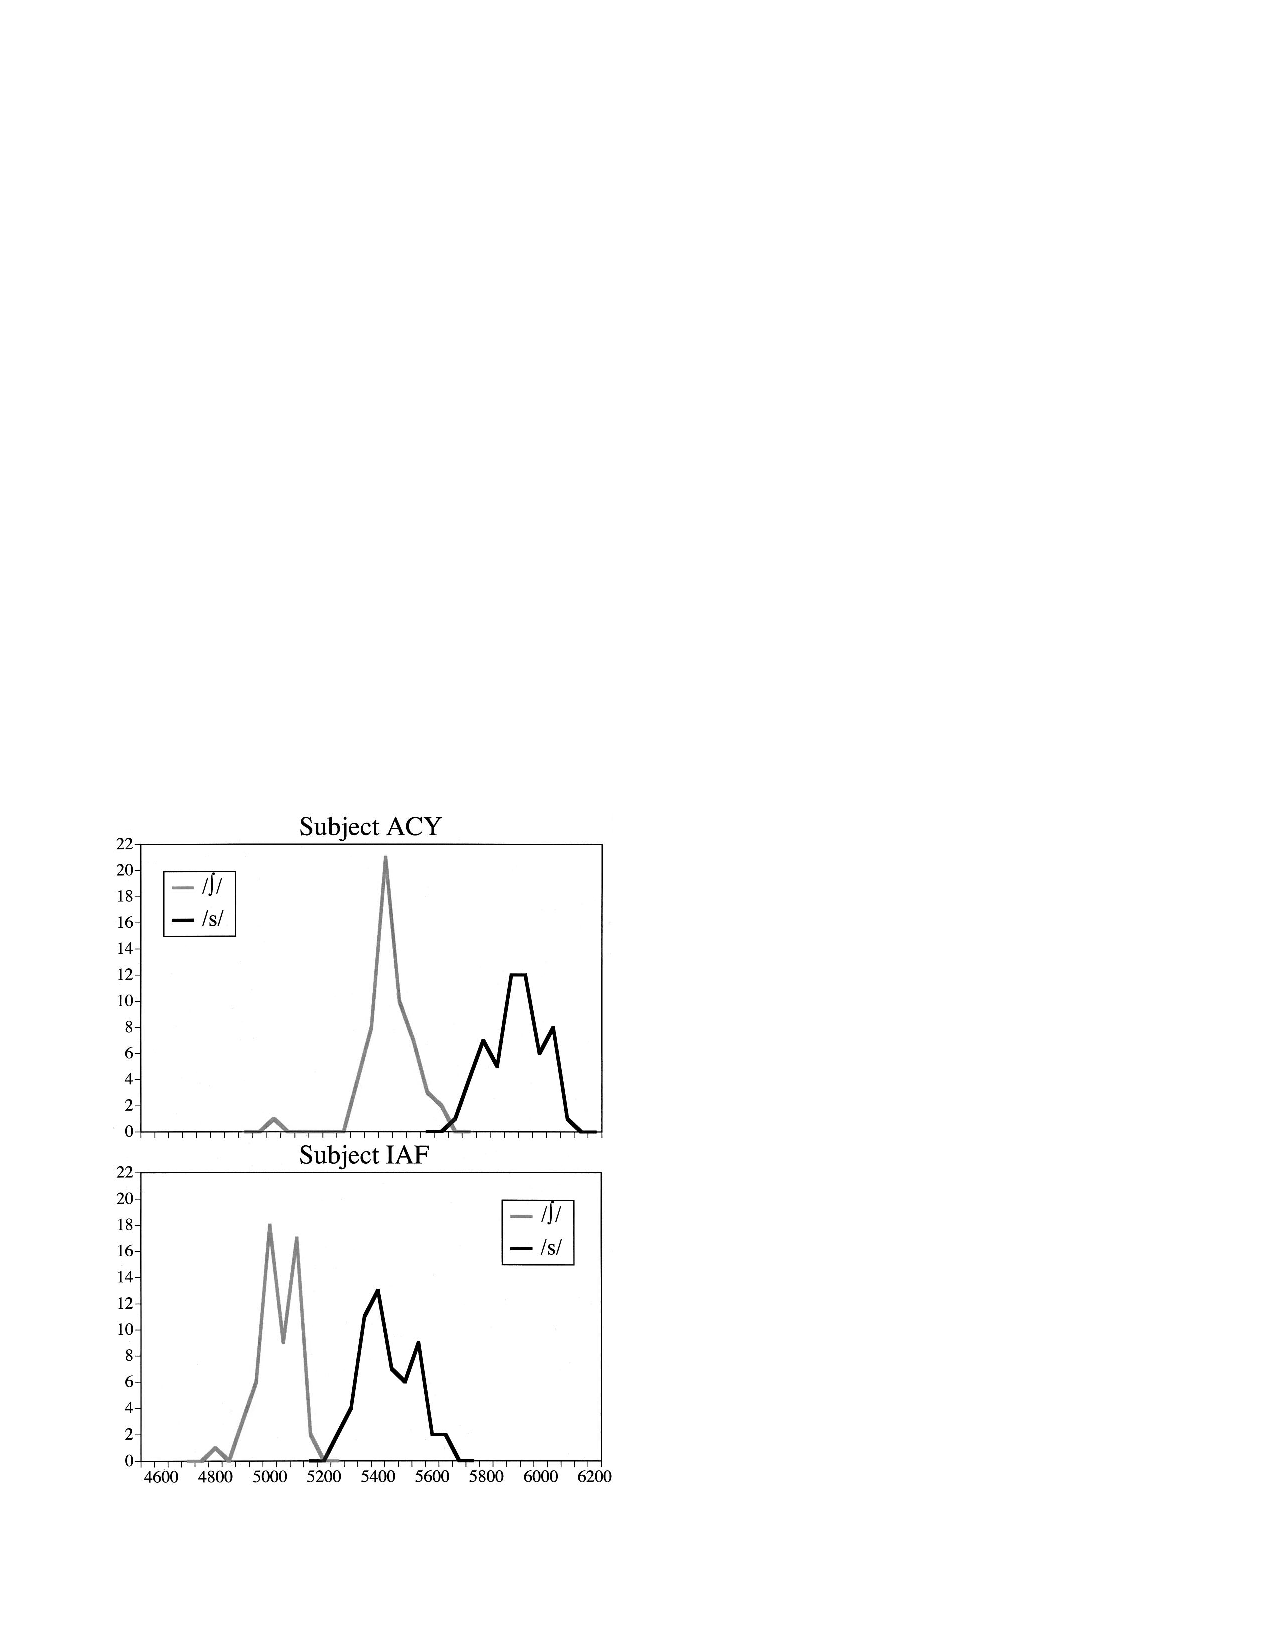
\includegraphics[width=0.5\textwidth] {newman-clouse-burnham-2001-fig2-categorical-mismatch.pdf}
  \caption{Distribution of frication frequency centroids, a crucial cue to the contrast between \ph s and \ph S, from two talkers \protect\autocite[reproduced with permission from][copyright 2001 Acoustical Society of America]{Newman2001}.}
  \label{fig:newman-et-al-fricative-centroids}
\end{figure}

\label{r3-environment-situation}
However, arguably the biggest challenge to speech perception is that the mapping from acoustic cues to phonetic categories can vary across situations. A `situation' could be characterized in terms of an individual talker or a group of talkers with a similar way of speaking, or other aspects of the environment which lead to systematic changes in speaking style (like a noisy bar). For example, different talkers sometimes realize even the same phonetic categories, in the same phonetic context, with dramatically differently cue distributions \autocite[e.g.,][]{Allen2003,McMurray2011a,Newman2001}.  These differences might arise from fixed, physical differences in, for instance, vocal tract size, but they also arise from variable or stylistic factors like language, dialect, or sociolect \autocite[e.g.,][]{Babel2014,Johnson2006,Labov1972,Pierrehumbert2003}.  These differences in the cue-to-category mapping can be substantial.
Figure~\ref{fig:newman-et-al-fricative-centroids} shows the distributions of one of the primary cues distinguishing between \ph s and \ph S as produced by two different talkers.  Such between-talker variability means that one talker's ``ship'' is physically more like another's ``sip''.
This problem is known as the \emph{lack of invariance} and is one of the oldest problems in speech perception \cite{Liberman1967}.
The focus of this article is how listeners manage to accommodate such systematic variability and achieve robust speech recognition.

\subsection{Overcoming the lack of invariance: The proposal}
\label{sec:overc-lack-invar}

In the face of the sort of variability between situations---talkers, in this case---seen in Figure~\ref{fig:newman-et-al-fricative-centroids}, it is natural to wonder how we can understand each other at all.  We propose that the answer to this question is three-fold:

\begin{enumerate}
\item recognize the familiar,
\item generalize to the similar, and
\item adapt to the novel.
\end{enumerate}

\label{r1-formalize-prev-work}
As we discuss below, at least the first and the last of these have been more or less explicitly assumed in previous work, and there is at least preliminary evidence for the second.  In a familiar situation, the speech recognition system has a great deal of previous experience to draw on, and by \emph{recognizing} a familiar situation it can take advantage of this previous experience. Recognition of the familiar underlies, for example, talker-specific interpretation of the acoustic signal \cite{Creel2008,Eisner2005,Goldinger1998,Kraljic2007,Nygaard1998}. Similarly, {\em generalizing} to a novel situation based on similar previous experience means the speech recognition system doesn't have to start from scratch each time a new situation is encountered. For example, such generalization allows us to recognize an accent and adjust our interpretations based on previous experience with similar talkers \cite{Baese-berk2013,Bradlow2008,Sidaras2009}. At the same time, novel situations might require adaptation beyond what is expected based on previous experience. For example, when encountering a talker with a novel dialect or accent, the speech recognition system must be prepared to \emph{adapt} rapidly and flexibly.

We propose that all three of these strategies arise from the function that the speech recognition system fulfills (i.e., the typical goals of speech recognition), and that the basic design of this system reflects the fact that it must function efficiently under normal
circumstances. Specifically, we propose that the three strategies emerge from the organizational constraints on the speech recognition system imposed by the presence of variability both within a single situation and between situations.  These constraints lead naturally to a few conceptual components for the proposed framework.  First, because there is variability within a situation, the mapping between cues and categories is inevitably \emph{probabilistic}. This makes speech recognition a problem of inference under uncertainty and implies that a robust speech recognition system must use distributional (statistical) knowledge \cite{Clayards2008,Feldman2009a,Norris2008}.

Second, because cue distributions themselves vary---sometimes unpredictably---across situations, the system must be prepared, when necessary, to engage in distributional/statistical learning.  This is closely related to the notion of life-long implicit learning \cite{Botvinick2004,Elman1990,Chang2006}, as well as statistical learning theories of language acquisition \cite{Feldman2013a,McMurray2009,Vallabha2007}, a connection we return to below.

Third, cue distributions do not vary arbitrarily across situations.  Rather, the world is structured.  For instance, a listener is likely to encounter a particular familiar talker's cue distributions again, relative to any arbitrary cue distributions, and likewise they are more likely to encounter cue distributions that are similar to those encountered in the past, because of regularities in how talkers vary within a language or more specific grouping like gender, dialect, accent, etc.  We propose that in order to take advantage of such structured variability, the speech perception system does not \emph{only} engage in distributional learning. In its most basic sense, this is demonstrated
by our ability to recognize previously encountered talkers, and use talker-specific experience to guide speech perception. 
Going beyond talker-specificity, we will discuss evidence that argues for sensitivity to structure over
\emph{groups} of talkers or situations. In a world where speech statistics vary in structured ways, life-long adaptation alone is not sufficient for robust speech perception. A robust speech perception system should take advantage of structure in the world that allows previous experience to inform current processing \autocite[for similar reasoning applied
to other cognitive domains, cf.][]{Qian2012}. It is, we propose, sensitivity to this structure in the world that underlies recognition of familiar situations and generalization to similar ones.

In this paper, we elaborate on this proposal, review the relevant literature, and develop a framework in the tradition of ideal observer models and normative/Bayesian inference \cite{Anderson1990} that, we hope, will help guide future work on speech perception. As we detail below, the proposed framework, which we dub the {\em ideal adapter}, understands all of (1) to (3) above (i.e., recognition, generalization, and distributional learning) as the result of selecting and adapting the appropriate generative model for the current situation based on the integration of prior and present experience (hence, the name for the proposed framework). 
This brings a unifying and---at least in parts---formalized computational framework to a set of ideas that have been assumed---more or less explicitly---by others before us. For example, it is widely assumed that speech perception is talker-specific \cite<e.g.,>{Creel2011,Pardo2006,Pisoni2007} and recent work has begun to investigate our ability to generalize across talkers \cite<e.g.,>{Bradlow2008,Eisner2005,Kraljic2007,Sidaras2009}. The ideal adapter framework ties together these different lines of work, emphasizing 
the crucial roles of both the structure of listeners' prior knowledge \emph{and} their ability to learn the statistics of novel situations. It has so far not been fully recognized, we submit, just how far-reaching the consequences of these two aspects of speech recognition are. Laying out the consequences of these two aspects of the framework thus forms the core of this article.

\label{r2-outline-parts}
We begin our exposition in Part I with adaptation to the novel. For this, we focus on situations in which listeners have high certainty (i.e., `know') that they need to adapt. We formalize the problem of adaptation and test the predictions of the ideal adapter framework through an implemented model.  We focus on two well-studied phonetic adaptation phenomena: the first where listeners recalibrate one phonetic category in response to auditorily ambiguous stimuli {\em labeled} as one category \autocite[perceptual recalibration or phonetic adaptation,][]{Bertelson2003,Kraljic2005,Norris2003}, and the second where listeners change their classification behavior after repeated exposure to the same prototypical stimulus \autocite[selective adaptation,][]{Eimas1973,Samuel1986}. This leads us to develop and test novel predictions of the proposed framework. In this part of the paper, we spend a substantial amount of time developing intuitions about the mechanics of how---in the ideal adapter framework---listeners can update their beliefs about the cue distributions in the current situation based on direct experience. In doing so, we illustrate how the proposed perspective relates to and diverges from standard accounts of speech recognition.

In Part II, we turn to situations where previous knowledge is crucial for robust speech perception: recognition of familiar situations and generalization to similar novel situations.  In contrast to the flexibility demanded by novel situations, in familiar situations listeners can benefit from \emph{stable} representations of past experience.  The ideal adapter framework provides a natural link between the distribution of speech statistics in the world---at the level of individual talkers and groups (e.g., dialect, gender, language)---and different strategies for how listeners can achieve robust speech perception in the face of the lack of invariance.  In Part II we will discuss what structure there is in the world that listeners can take advantage of and review the evidence that they \emph{do} take advantage of it. In doing so, we identify directions for future research and isolate a number of specific questions that we consider particularly critical for our understanding of the human speech recognition system.

Finally, we close in Part III by putting the framework we have developed into broader perspective.  In particular, we will address how our approach relates to other approaches to the problem of the lack of invariance.  Following that, we will discuss how our framework might inform broader issues in speech perception, language comprehension, and more domain-general learning and adaptation. Our approach is a computational-level one and as such compares only indirectly to mechanistic- or algorithmic-level approaches \cite{Marr1982}, but it nevertheless provides a set of tools for reasoning about speech perception (and language comprehension more generally) which can help sharpen questions for research at other levels.  For example, the questions raised by the ideal adapter framework also speak to the debate between episodic, exemplar-based or more abstract phonetic representations \cite{Johnson1997,Goldinger1998,McClelland1986,Norris2008,Pierrehumbert2003}. They also relate to the acquisition of phonetic categories, which can be seen as another type of distributional learning problem \cite{Maye2002,McMurray2009,Vallabha2007}, and to language processing at higher levels \cite<e.g.,>{Fine2013,Grodner2011,Kamide2012,Kurumada2012,Kurumada2014}.  We also discuss recent research that has found adaptive behavior in language processing above the level of speech perception. At its most basic, the ideal adapter framework also contributes to the burgeoning literature on learning in a variable world \autocites[e.g., change detection][]{Gallistel2001}[hierarchical reinforcement learning][]{Botvinick2012}[motor learning][]{Kording2007a}.  Along with other recent approaches, the ideal adapter stresses that the cross-situational statistics of the world---though being variable---are \emph{structured}, and that our cognitive systems have evolved to take advantage of this structure.
\label{r2-outline-parts-end} 

\section*{Part I}
\label{sec:part-i}

\section{The ideal adapter framework}
\label{sec:framework}

Adaptation in speech perception has received a great deal of attention recently. For example, when listeners initially encounter accented speech, they process it more slowly and less accurately, but this disadvantage dissipates within a matter of minutes \autocite[][and references therein]{Bradlow2008,Clarke2004}. Similarly, listeners rapidly adapt to synthesized and otherwise distorted speech \autocite[e.g.,][]{Davis2005}. Adaptation is not limited to cases of highly unusual pronunciation, such as foreign accents. Even relatively subtle divergences from standard cue distributions can lead to adaptation.  For example, listeners adapt to a talker who produces cue distributions with a typical mean value but less variability than normal \cite{Clayards2008}.  This suggests that continuous and implicit adaptation to subtle deviations from auditory expectations is a pivotal component of the human speech perception systems.

What is lacking thus far, however, is a better understanding of \emph{how} and \emph{when} we adapt.  Specifically, how do listeners detect that their current linguistic representations are inadequate for the current situation, and how is evidence from the currently processed speech stream integrated with previous experience in order to achieve adaptation?   Despite the central importance of the lack of invariance problem to speech perception and language understanding \cite{Liberman1967,Pardo2006}, to date there are few cognitive models of adaptation, and as we discuss below, those that do exist do not link it to other strategies for dealing with the lack of invariance.  State of the art models of speech perception have begun to address the non-determinism inherent in the mapping from cues to categories, but ignore or abstract away from the specific contributions of the lack of invariance \cite{Feldman2009a,Feldman2013a,Norris2008}.\footnote{In work on automatic speech recognition, however, the interest in talker-independent speech recognition has led to a range of proposals that are similar in varying degrees to what we propose here for human speech recognition \autocite[e.g.,][]{Gauvain1994,Leggetter1995,Shinoda2001}.}

We propose that the first important step is to ask {\em why} phonetic adaptation occurs at all, or rather why one would expect speech perception to exhibit adaptive properties.
To that end it is helpful to understand speech perception as a problem of inference under uncertainty.
The acoustic cues that provide information about the talker's intended message are variable and ambiguous, and thus each individual cue is only partially informative.
In order to effectively infer the underlying message, information must be integrated from many sources, and as we will discuss below, this must be guided by knowledge of the distribution of cues associated with each linguistic unit.  However, because of the lack of invariance, these distributions differ across situations (e.g., talkers).

\subsection{Adaptation through belief updating}
\label{sec:robust-speech-perc}



Our central proposal is twofold.  First, listeners do not have direct access to the true distribution but rather uncertain \emph{beliefs} about them based on a limited number of observations.  Second, inaccurate beliefs about the underlying distributions can lead to slowed or inaccurate phonetic categorization, and in order to achieve robust speech perception across situations, listeners must adapt.  In this view, adaptation reflects a sort of incremental distributional learning,
and such distributional learning can be computationally characterized as \emph{belief updating}. This incremental distributional learning has to integrate recent experience with a novel situation with prior knowledge and assumptions about the language. In this sense, the proposed account builds on and expands on the general idea of life-long implicit learning \cite{Botvinick2004,Chang2006,Elman1990} and that the processing of language input is inevitably tied to implicit learning \autocite[e.g.,][]{Clark2013,Dell2014,Jaeger2013a}. Unlike much of this work, however, we will argue that the implicit beliefs listeners hold based on previous experience are not unstructured. Rather, they reflect higher-level knowledge (beliefs) about different talkers, groups of talkers, dialect and accents, and so on.  We return to this in the second part of the paper.

The first proposition of our framework is that human speech perception relies on a \emph{generative model}, or the listener's knowledge of how linguistic units (words, syllables, biphones, phonetic categories, etc.) are realized by different distributions of acoustic cues.  Such knowledge allows for speech perception to proceed by comparing how well each possible explanation---higher-level linguistic unit---\emph{predicts} the currently observed signal.  The proposal that language comprehension proceeds via prediction of the signal accounts for a variety of properties of language understanding beyond the ones discussed here \autocite[cf.][]{Dell2014,Farmer2013,Jaeger2013a,MacDonald2013,Pickering2013} and is closely related to similar proposals from visual perception and other domains \cite{Clark2013,Friston2005,Hinton2007,Huang2011,Rao1999}.

\label{r1-cues-depend-who}
Our second proposition is that the cue values predicted from a given linguistic unit depend not only on what is being said (the phonetic category, biphone, word, etc.) but also on \emph{who} is saying it, and good speech perception depends on using an appropriate generative model for the current talker, register, dialect, etc..  The listener never has access to the \emph{true} generative model, but rather only their uncertain \emph{beliefs} about that generative model.  Thus, adaptation can be thought of as an update in the listener's talker- or situation-specific beliefs about the linguistic generative model.  The idea that speech adaptation reflects learning about the linguistic generative model is not in and of itself novel, but it has largely been implicit in the empirical literature thus far and our proposal provides an explicit framework and formalization for understanding the link between learning and processing in speech perception.

Our goal is to provide a framework for understanding, on the one hand, how listeners might best represent past experience with different situations, and on the other hand how listeners can integrate that previous experience with evidence from the currently processed speech signal in order to infer an appropriate generative model for each situation.  As we discuss below, the listener needs to bring their beliefs about the distribution of cue values for each category into alignment with the actual distribution that the talker is producing.  Because the speech signal unfolds over time, and because the fine-grained acoustic information fades rapidly, this belief updating must be done incrementally. However, this is difficult because each individual speech sound is corrupted by the intrinsic variability
of the speech production, transmission, and perception process, and hence not an unambiguous cue to the underlying distribution.  That is, when a listener hears a cue value that they do not expect, it could be due either to a change in the underlying distributions,
or because deviations from prototypical cue values happen for a variety of other reasons (muscle fatigue, coarticulation, background noise, etc.).  The question is thus how the listener should incorporate each new piece of evidence into their beliefs.  We address this question by developing an \emph{ideal adapter} framework, which, in the tradition of computational-level/rational analysis \cite{Anderson1990,Marr1982}, sets out the statistically optimal way to do this integration. By this, we mean that adaptation reflects an inference process which combines prior beliefs and recent experience proportional to the degree of confidence in each.\footnote{This is not intended as a claim that such inference is resource-free or that there is unlimited memory. Importantly, there are many cognitively plausible algorithms which provably approximate---in principled ways---the type of rational inference assumed here for simplicity's sake, and do so with limited resources \cite<e.g.,>{Sanborn2010}. Many of these algorithms are closely related to mechanistic models like exemplar models \protect\autocite[see][]{Gibson2013,Shi2010}. We return to this point in the final part of this article.}


\subsection{The ideal listener or phonetic categorizer}
\label{sec:ideal-phon-categ}

Our ideal adapter framework builds on a foundation of {\em ideal listener} models, which describe the problem of speech perception as statistical inference of the talker's intentions \cite{Clayards2008,Feldman2009a,Norris2008,Sonderegger2010}. Such inference includes inferring intermediate linguistic units, like phonetic categories, either as a means to another end or as an end in itself, as in the case of explicit experimental phonetic categorization tasks.  Because we focus specifically on the problem of inferring phonetic categories, for our purposes an ideal listener model is better characterized as an {\em ideal phonetic categorizer} model. For the broader goal of understanding speech perception, it should, however, be kept in mind that the human listener is not just a phonetic categorization machine, and phonetic categorization typically serves other ends \autocites[such as lexical access,][]{Norris2008}[or even the successful inference of communicative intentions][]{Jaeger2013b}.

Because of the inherent variability of how a phonetic category is realized acoustically, any particular cue value is in principle ambiguous, and thus phonetic categorization is a problem of inference under uncertainty.  Such inference can be formally expressed in the language of Bayesian statistics.  In the general case, the posterior probability of each category $C=c_i$ after observing cue value $x$ is related to the \emph{prior probability} of $c_i$,  $p(C=c_i)$ and the \emph{likelihood} of $x$ under category $c_i$, $p(x|C=c_i)$, according to Bayes rule:
\begin{equation*}
  p(C=c_i | x) = \frac{p(x | C=c_i) p(C=c_i)}{\sum_j p(x|C=c_j) p(C=c_j)}  % |
\end{equation*}
Because the denominator of the fraction does not depend on the specific category $c_i$ and only serves to ensure that all of the posterior probabilities $p(C=c_i | x)$ sum up to one, it is often omitted and the relationship is written as proportionality:
\begin{equation*}
  p(C=c_i | x) \propto p(x | C=c_i) p(C=c_i)
\end{equation*}

\begin{figure}[htb]
  \centering
  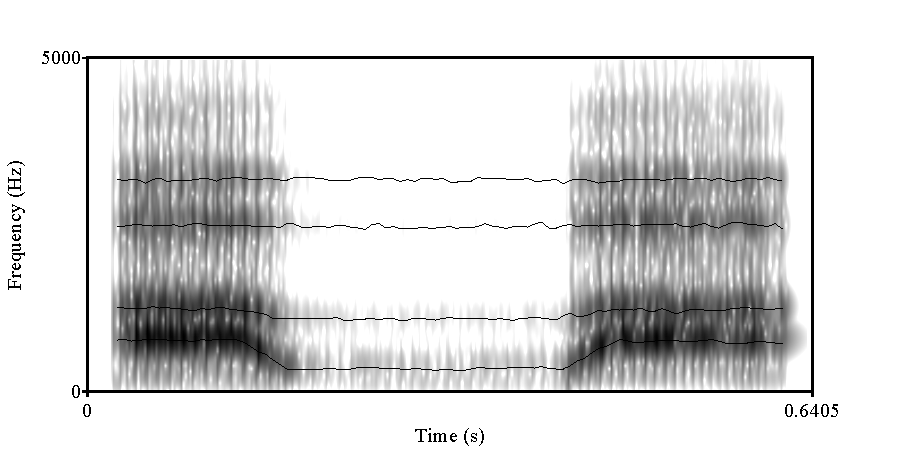
\includegraphics[width=0.6\textwidth]{figs/vroomen-aba-spectrogram-tracks.pdf}
  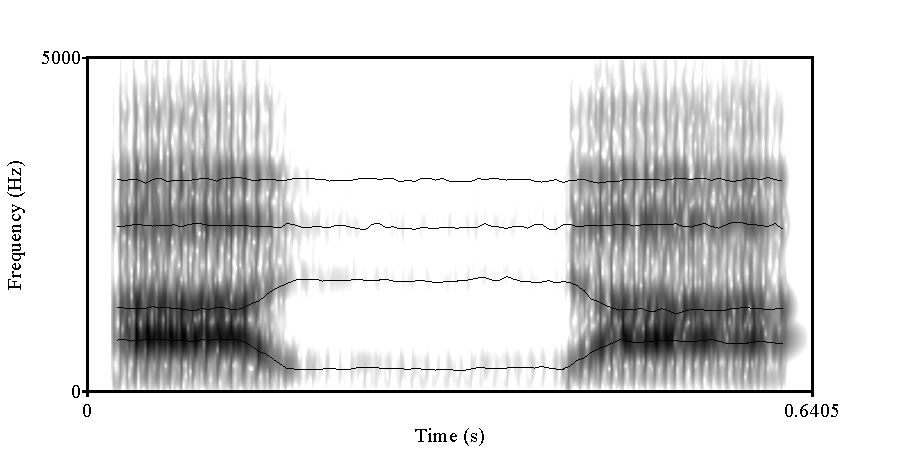
\includegraphics[width=0.6\textwidth]{figs/vroomen-ada-spectrogram-tracks.pdf}
  \caption{Spectrograms for \ph{aba} (top) and \ph{ada} (bottom) with formant tracks (synthesized as described in \protect\citeA{Vroomen2004} and provided by Jean Vroomen).  Note the higher second formant (F2) locus for the transitions into and out of the closure for \ph{ada}.}
  \label{fig:aba-ada-spectrograms}
\end{figure}

In this paper, we will begin by addressing a very simplified phonetic categorization problem, in which the listener is trying to decide whether a given cue value is a \ph b or \ph d, and later discuss how the approach we develop applies in general.
One important cue to this phonetic contrast is the F2 locus, or ``target'' of the second formant transition \cite{Delattre1955}.  Figure~\ref{fig:aba-ada-spectrograms} shows the spectrograms corresponding to synthesized \ph{aba} and \ph {ada} tokens \autocite[synthesized by][]{Vroomen2004}.  Figure~\ref{fig:dist-id-schematic} (left panel) shows schematically how the distributions of F2 loci differ for \ph b and \ph d: \ph b typically has a lower F2 locus, but there is some variability for both \ph b and \ph d.  There is thus a continuum from \ph b-like to \ph d-like F2 locus values.

Let's assume for simplicity's sake that the listener is only considering F2 locus as a cue to the \ph b-\ph d contrast.  Given an observed \ftwolocus value, the listener must infer how likely it is that the talker intended to produce the phonetic category $C=$\ph b.  That is, what is the posterior probability $p(C=\mrb \given \ftwolocus)$?\footnote{Here and elsewhere, we write ``\mrb'' for ``\ph b'' in equations, for the sake of brevity.  We also write $p(\mrb)$ to indicate $p(C=\mrb)$.}  This quantity is found via Bayes rule:
\begin{align}
  \label{eq:1}
  p(\mrb \given \ftwolocus) &= \frac{p(\ftwolocus \given \mrb) p(\mrb)}{p(\ftwolocus \given \mrb) p(\mrb) + p(\ftwolocus \given \mathrm d) p(\mathrm d)} \\
  &=\frac{p(\ftwolocus \given \mrb) p(\mrb)}{p(\ftwolocus)} \\
  \label{eq:2}
  &\propto p(\ftwolocus \given \mrb) p(\mrb)
\end{align}

Bayes rule captures the fact that the posterior probability depends on three things.  First, it depends on the \emph{prior probability} of the hypothesis, $p(\mrb)$, which could be higher if \ph b is more frequent in the language than \ph d, or if there are other contextually available sources of information that make \ph b more likely, like lexical, visual, or coarticulatory cues.  Second, it depends on the \emph{likelihood} $p(\ftwolocus \given \mrb)$, which is the probability of the observed \ftwolocus value given that \ph b was intended by the talker.  Finally, it also depends on how credible \emph{other} hypotheses are, which is really a consequence of requiring that the posterior probabilities of all hypotheses add up to one.  This is equivalent to the overall probability of the observed \ftwolocus value, regardless of which hypothesis is true, and since this quantity is the same for all potential hypotheses it is frequently omitted, as in \eqref{eq:2}.

For an ideal listener, the probability of recognizing a \ph b should be the estimate of the posterior probability of \ph b (and likewise for \ph d) \cite{Clayards2008,Feldman2009a}.  This assumes that the result of speech recognition is not a single category but rather uncertain (or variable) estimates of which categories are more or less likely.  This is not a trivial assumption. For example, one might imagine that a listener would improve its categorization accuracy by always `guessing' the category with the highest probability.  However, for speech perception more broadly, there is a benefit to maintaining uncertainty about the category, since additional information often becomes available later in the speech signal (e.g., because of the asynchronous nature of acoustic cues). Indeed, human listeners seem to maintain uncertainty about the speech signal for at least a limited amount of time \autocite[cf., right-context effects in word recognition,][]{Bard1988,Connine1991,Dahan2010,Grosjean1985}

Treating speech perception as inference under uncertainty provides substantial insight.  Much of this comes from the fact that in such a framework, recognition is accomplished not through purely bottom-up template matching but rather by comparing how well each possible higher-level explanation can \emph{predict} the input signal.
This framework provides accounts of effects such as the perceptual magnet effect \cite{Feldman2009a}, compensation for coarticulation \cite{Sonderegger2010}, and integration of auditory and visual cues \cite{Bejjanki2011}.  It also describes speech and language processing at other levels, including lexical access \cite{Norris2008}, the incremental integration of words into a syntactic parse \cite{Hale2001,Levy2008,Levy2008a}, and pragmatic reasoning \cite{Frank2012,Goodman2013}
Moreover, Bayesian inference has been shown to provide a powerful and general computational framework for describing statistically optimal inference under uncertainty, via the integration of prior beliefs and recently observed data.  This perspective thus extends to other perceptual and cognitive domains \cite{Griffiths2010,Kersten2004,Tenenbaum2001}, including sensory adaptation in non-language domains \cite{Fairhall2001,Kording2007a,Stocker2006}.

One specific advantage of this framework for understanding phonetic adaptation is that it links speech perception behavior with the distribution of cues associated with each category.
For an ideal listener, the classification curve for /b/ and /d/ responses is derived directly from the respective posterior probabilities (Figure~\ref{fig:dist-id-schematic}, left panel), which in turn are computed in part from the corresponding likelihood, or distribution, function for each category:
\begin{equation}
  \label{eq:3}
  p(\mathrm{response} = \mrb \given \ftwolocus) = p(\mrb \given \ftwolocus) \propto p(\ftwolocus\given\mrb) p(\mrb)
\end{equation}
Indeed, listeners do appear to use distributional information in speech perception.  \citeA{Clayards2008} found that listeners adapt to specific distributions of auditory cues to \ph b and \ph p.  Listeners in this experiment performed a spoken-word picture identification task, where some of the stimuli were \ph b-\ph p minimal pairs like ``beach'' and ``peach''.  Listeners were randomly assigned to two conditions. In both conditions, the \ph b and \ph p percepts were drawn from normal distributions over the primary acoustic cue to the \ph b-\ph p contrast \autocite[voice onset timing, VOT,][]{Lisker1964}.  In the high-variance condition, the variance around the VOT category means for \ph b and \ph p was large; in the low-variance condition, it was small.  Listeners' classification boundaries reflected the distribution of cues that they experienced: for low-variance exposure, the classification boundaries were steep, while for high-variance exposure the boundaries were shallower, reflecting the greater uncertainty about the intended category that comes with more variable productions of each category.  Moreover, the difference in boundary slopes was quantitatively predicted by the difference in the category variances in each case.

This result demonstrates two points.  First, by showing that listeners' categorization boundaries reflect the variance of the talker's VOT distributions as predicted by the ideal listener model, they show that listeners are using probabilistic cues in a nearly optimal way.  Second, and more importantly for our purposes, they show that listeners are \emph{adapting} to a change in the statistics of these cues.  Because they have no experience with the experimental talker before beginning the experiment, any differences in their classification function after exposure reflects something that they have learned about the talker's VOT distributions over the course of the experiment.

The natural question to ask is: \emph{how} do listeners get to the point where distributional information is reflected in their behavior?  Intuitively, we might say that coming into a new situation---like an experiment---listeners have some beliefs about the distributions of cues for each phonetic category, and that these beliefs change as the listener gains more experience in that situation.  These changes in beliefs about how cues are distributed leads to changes in how any given cue is interpreted, resulting in possibly better comprehension or changes in classification behavior.  In the next section we show how---like phonetic categorization---this intuitive idea formally corresponds to statistical inference, but at a different level.

\subsection{The ideal adapter}
\label{sec:ideal-adapter}

Our ideal adapter framework builds on the ideal listener framework described in the last section.  The ideal listener depends on distributional information about each category, in the form of the likelihood function $p(x \given C)$.
We can think of the likelihood function for each category as the listener's prediction about what cue values are likely to occur given that category is produced, and this prediction is used during speech perception to evaluate how well each hypothesized category explains the particular cue value currently being classified.  However, we can also think of the likelihood functions as explanations of (and predictions about) the \emph{statistics} of cues for each category.  Crucially, these explanations come from the listener's \emph{subjective} knowledge of cue distributions, and likely are not exactly identical to the true statistics of cues in the world, because a listener only has finite observations to work with and thus incomplete information about the true distributions.  The consequence of this is that the listener has \emph{uncertain} knowledge of cue distributions.

If the statistics of cues associated with each category were identical or at least similar from one situation to the next, information could be accumulated from \emph{all} observed values to obtain sufficiently accurate---and certain---estimates of the likelihood function.
But as discussed above, this is not always the case: talkers can differ dramatically in the acoustic cues they use to realize phonetic categories, and thus the true likelihood function differs across situations \cite{Allen2003,Labov1972,Hillenbrand1995,McMurray2011a,Pierrehumbert2003}.

\begin{figure}[t]
  \centering
  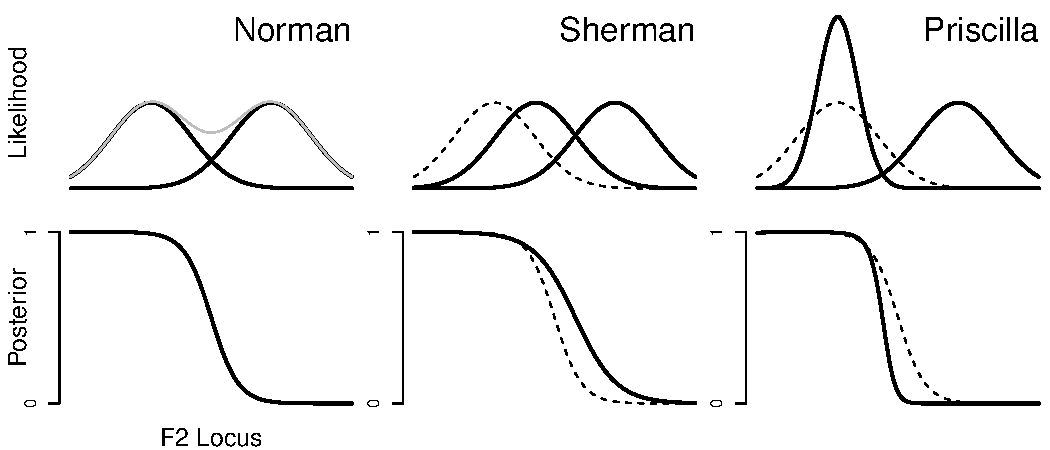
\includegraphics[width=\textwidth]{figs/dist-id-shift-var-schematic.pdf}
  \caption{Relationship between F2 locus likelihood functions $p(x | c)$ (top) and posterior probability of \ph b, or classification function $p(c | x)$ (bottom; assuming $p(c)=0.5$ for both $c=$\ph b and \ph d), for three different talkers: a `normal' talker (Norman), a `shifted' talker (Sherman), and a `precise' talker (Priscilla).  Dashed lines show the \ph b likelihood function and classification function corresponding to the `normal' talker.  Light gray line in top left shows the marginal likelihood, $p(x) = \sum p(x | c) p(c)$, which corresponds to the overall distribution of cue values, regardless of which category they came from, and is the sum of the two likelihood functions.}
  \label{fig:dist-id-schematic}
\end{figure}

In order to make good use of bottom-up information from acoustic cues,
listeners require the appropriate likelihood function for the current situation.
Consider again the case of making a \ph b-\ph d decision on the basis of the F2 locus cue, but suppose that we have encountered a new talker---call him Sherman---who produces a different distribution of F2 locus values for \ph b, a distribution which is shifted to the right (Figure~\ref{fig:dist-id-schematic}, middle).  If the listener continues to use the likelihood function which matches the `normal' talker Norman's \ph b distribution, comprehension of Sherman's speech will suffer: cue values which were ambiguous for Norman are now more likely to be generated from \ph b (middle bottom; the ideal classification function for Sherman, the solid line, is above the dashed line).  Conversely, cue values that are perfectly ambiguous for Sherman (where the solid line crosses $p(\mrb \given \ftwolocus)=0.5$) would be much more likely to be \ph d when produced by Norman.  That is, a mismatched likelihood function can result in slowed or inaccurate comprehension: inaccurate because the ideal category boundary depends on the likelihood function, and slower because \ph b cue values which are nearly prototypical and highly likely for the new talker would be ambiguous for the standard talker \autocite[the resulting uncertainty slows processing in this sort of task;][]{Clayards2008,McMurray2002}.

Similarly, consider the third talker in Figure~\ref{fig:dist-id-schematic} (right), Priscilla, whose \ph b productions are substantially more precise than Norman's, resulting in a low-variance cue distribution for \ph b, but whose \ph d productions show normal variability.  Using Norman's likelihood function to classify Priscilla's productions has similar consequences in this situation: cue values that would have been ambiguous for Norman are now quite a bit more likely to have come from the \ph d distribution because Priscilla's \ph bs are so precise.

In both of these situations, comprehension difficulties could be avoided if the listener could use the right likelihood function.  If the talker is familiar, this might be as simple as retrieving the right likelihood function based on prior experience with the talker \cite<cf.>{Goldinger1998}.\footnote{There is the additional problem of detecting {\em that} the distributions have changed. Change detection in a probabilistic task is a difficult problem that has so far received little attention in research on speech perception and language processing, but has been investigated for other cognitive domains \cite<for a review of the literature, see>{Qian2012} and in research on automatic speech recognition \cite<e.g.,>{Ajmera2004,Chen1998}. As we outline in the second half of this article,  the framework we propose holds the potential of a unified solution to both adaptation and change detection.}
But what if the talker has never been encountered before?  This is a distributional learning problem: in order to achieve efficient and accurate comprehension of a novel talker, the listener must learn the cue distributions corresponding to the new talker's phonetic categories.  This is similar to the problem faced by an infant acquiring their first language, although the adult listener starts with a substantial amount of prior knowledge.  Most notably, they know that there \emph{are} different phonetic categories for \ph b and \ph d, and that these categories are generally distinguished by the F2 locus cue.  As we discuss in the second half of this article, adult listeners also may have experience with similar talkers, providing them with more or less useful previous experience.

Still, inferring the distributions of F2 locus values corresponding to these categories is a difficult task, because the inherent variability in these distributions makes each observed cue value ambiguous as evidence for the underlying distribution: if the observed cue value deviates from the listener's predictions, is it due to inherent within-category variance (which will produce \emph{some} outliers), or is it evidence that the predictions themselves---the likelihood functions---are wrong and need to be updated?

Thus, determining the talker's category distributions is a problem of inference under uncertainty, just like the problem inferring the talker's intended category based on an observed cue value, but at another level.  That is, in the same way that the listener can use their knowledge of how well each possible category predicts an observed cue value to infer which category is most likely, they can also use knowledge about how well each possible category \emph{distribution} predicts the observed statistics of their recent experience in order to infer which underlying distributions are more or less likely in the current situation.  The statistically optimal solution to this inference problem can again be described using Bayes Rule.  For simplicity's sake, the cue distribution\footnote{Here we are representing categories as Gaussian (normal) distributions, because they are both mathematically and intuitively tractable.  This assumption is not critical for our purposes.  The same logic---of belief updating as inferring distributional properties---applies for any parametric or even non-parametric way of representing the distributions.} for a category $c$ can be represented by its mean $\mu_c$ and variance $\sigma_c^2$.  Thus the listener's uncertain \emph{beliefs} about this cue distribution can be represented by a probability distribution over means and variances.

An ideal adapter must infer \emph{both} the category label $c$  \emph{and} and the means and variances of the different underlying categories $\boldsymbol\mu, \boldsymbol\sigma^2 = \{\mu_c, \sigma^2_c\}$ (where for our example, $c=/\mrb/, /\mrd/$).  Formally, this is expressed by the \emph{joint} posterior distribution over category labels and means and variances, which combines prior beliefs with the likelihood of the observed evidence:\footnote{Using the shorthand notation of $p(c)$ to indicate the probability that the random variable $C$ has value $c$, or $p(C=c)$.}
\begin{equation}
  \label{eq:12}
  p(c, \boldsymbol{\mu}, \boldsymbol{\sigma}^2 \given x) \propto
  \underbrace{p(x \given \mu_c, \sigma^2_c)}_\mathrm{likelihood}
  \underbrace{p(c) p(\boldsymbol{\mu, \sigma}^2)}_\mathrm{prior}
\end{equation}
This captures the fact that after observing a cue value $x$, the listener's joint beliefs about the intended category $C=c$ and the parameters of all categories $\boldsymbol{\mu, \sigma}^2$ depend on two things.  First, the updated beliefs depend on the likelihood, how well each possible combination of categorization and category parameters can predict the observation $x$, $p(x \given c, \boldsymbol{\mu, \sigma}^2) = p(x \given \mu_c, \sigma^2_c)$.  Second, they depend on the listener's prior beliefs, both about which categories are most likely to be encountered, $p(c)$, \emph{and} which combinations of category means and variances are most probable, $p(\boldsymbol{\mu,\sigma}^2)$.  Both aspects of the prior are based on prior experience.  The prior over category probabilities depends on the base rate for each category, as well as its probability in context (based on the surrounding sounds or word, or other acoustic cues besides $x$),\footnote{The usefulness of context in providing prior information about phonetic categorization is not limited to situations where the categorization of nearby sounds is known with certainty.  Simply knowing that sequences of categories which correspond to actual words are more likely than arbitrary strings provides prior information about how each sound is categorized through the joint distribution of categorizations $p(\ldots, c_{i-2}, c_{i-1}, c_i, c_{i+1}, \ldots)$.} while the prior over category means and variance depends on the sorts of cue distributions the listener has encountered before and expects to encounter again.  The nature of the prior over category means and variances is the focus of Part II below.  For now all that matters is that the listener thinks some category means and variances are more likely than others.

The specific way that an ideal adapter updates their beliefs after observing cue value $x$ depends on how they categorize it, and this is captured by the joint posterior distribution $p(c, \boldsymbol{\mu, \sigma}^2 \given x)$.  In general, an observation from category $c$ provides the most evidence about the underlying mean and variance of that category.  In the case where the prior beliefs about the parameters of each category are independent of each other, $p(\boldsymbol{\mu, \sigma^2}) = \prod_c p(\mu_c, \sigma^2_c)$, the beliefs about category $c_i$ are \emph{only} updated if the observation is classified as $C=c_i$.
\begin{equation}
  \label{eq:20}
  p(\mu_{c_i}, \sigma^2_{c_i} \given x, C) \propto
  \left\{
    \begin{array}{lr}
      p(x\given \mu_{c_i}, \sigma^2_{c_i}) p(\mu_{c_i}, \sigma^2_{c_i}) & \textrm{if } C=c_i  \\
      p(\mu_{c_i}, \sigma^2_{c_i}) & \textrm{if } C \neq c_i
    \end{array}
  \right.
\end{equation}

In cases where there is uncertainty about how the observation $x$ should be categorized, an ideal adapter should update the beliefs about category $c_i$ as a mixture of the updated beliefs under each possible categorization, weighted by how likely that categorization is overall (averaging or marginalizing over current category parameter beliefs):
\begin{equation}
  \label{eq:18}
  p(\mu_{c_i}, \sigma^2_{c_i} \given x) = \sum_c p(\mu_{c_i}, \sigma^2_{c_i} \given x, C=c) p(C=c \given x)
\end{equation}
Again, if we assume that the beliefs about different categories are independent, this mixture consists of two components: one where $x$ is categorized as $C=c_i$ and beliefs about category $c_i$ are updated, and one where it is not and no belief updating occurs:\footnote{In the general case where the prior beliefs about different categories' parameters are not independent, the posterior is still a mixture, but is a mixture of beliefs, updated in different ways and to different extents, rather than just updated and non-updated beliefs.}
\begin{align*}
  \label{eq:19}
  p(\mu_{c_i}, \sigma^2_{c_i} \given x) =&\ p(\mu_{c_i}, \sigma^2_{c_i} \given x, C=c_i) p(C=c_i \given x) \\
  &+ p(\mu_{c_i}, \sigma^2_{c_i}) p(C \neq c_i \given x)
\end{align*}

To return to the example above of classifying a token as either \ph b or \ph d based on F2 locus, the posterior distribution over the mean and variance of \ph b after observing a particular \ftwolocus value is thus
\begin{align*}
  p(\mu_\mrb, \sigma^2_\mrb \given \ftwolocus) = &\  p(\mu_\mrb, \sigma^2_\mrb \given \ftwolocus, \mrb) p(\mrb \given \ftwolocus) \\
&+ p(\mu_\mrb, \sigma^2_\mrb) p(\mrd \given \ftwolocus)
\end{align*}

In conversational speech, acoustic observations are often labeled with high certainty, and so $p(C=c_i \given x) \approx 1$ for some category $c_i$.  Such label information can come both from top-down linguistic context (like phonotactics or lexical disambiguation), or from other bottom-up cues.  For example, when distinguishing \ph b from \ph d, the closure of the lips during \ph b provides a very informative visual cue, effectively labeling the auditory percept \cite{Vroomen2004}.

In such cases where there is some other source of information that labels the observed \ftwolocus value as a \ph b, the resulting conditional posterior distribution over the mean and variance of \ph b simplifies to:
\begin{equation}
  \label{eq:10}
  p(\mu_\mrb, \sigma^2_\mrb \given \ftwolocus, \mrb) \propto
  \underbrace{p(\ftwolocus \given \mrb, \mu_\mrb, \sigma^2_\mrb)}_\mathrm{likelihood}
  \underbrace{p(\mu_\mrb, \sigma^2_\mrb)}_\mathrm{prior\ beliefs}
\end{equation}
Here, the relevant prior distribution is just the listener's prior beliefs about the mean and variance of the \ftwolocus cue for the \ph b category.  Likewise, the likelihood considers only how well each combination of \ph b mean and variance account for the observed cue value.  Below, we model incremental adaptation for cases where the category labels are known with high certainty (and thus \eqref{eq:10} holds).  We also assume that the prior beliefs about \ph b and \ph d are independent.  We make these assumptions for the sake of simplicity and tractability in modeling, and it is important to keep in mind that they do not represent assumptions of the \emph{framework}, which makes qualitatively the same predictions whether or not these assumptions turn out to be true.

In sum, the ideal adapter framework predicts that optimal phonetic adaptation depends on three things: the statistics of the observed percepts (e.g. their mean and variance), the listener's prior beliefs about the statistics of the relevant categories, and the listener's belief that there is a need to adapt (including their beliefs about the amount of variation in the relevant category across talkers and situations). In the next five sections, we illustrate the role of the first two factors in phonetic adaptation experiments where the third factor is a given \autocite[i.e., where there is a clear need to adapt and for which previous work has shown that listeners indeed adapt,][]{Bertelson2003,Kraljic2005,Norris2003}.  In order to do this we specify a basic belief updating model in the ideal adapter framework which quantifies how the exposure statistics and the listener's prior beliefs about those statistics interact.

With this model in hand, we do five things.  First, as a basic evaluation we address the phenomenon of phonetic recalibration or perceptual learning. %(Section \ref{sec:model-recal})
Such perceptual learning is typically thought to be due to changes in the underlying representations of the adapted categories which generally serves the purpose of robust speech perception, and is naturally accounted for by the ideal adapter framework.  In particular, we show that the incremental build-up of recalibration is accounted for by our basic belief updating model.

Second, we illustrate how the way in which the model accounts for the build-up of recalibration potentially sheds light on the underlying processes. %(Section~\ref{sec:recal-categ-shift}).
Specifically, the model captures the fact that recalibration is often ambiguous between a change in the underlying mean of the category versus a relaxation of the criterion for what counts as an acceptable exemplar, or a change in the variance of the category.

Third, we examine the predictions of this framework for the selective adaptation paradigm, a paradigm which is typically \emph{not} considered to be due to the perceptual learning which serves robust speech perception.  However, we show that the belief updating model accounts for the incremental build-up of this phenomenon as well, using very similar parameters as for recalibration.

Fourth, we explore a little studied property of phonetic recalibration that, {\em prima facie}, would seem to stand in conflict with our hypothesis that adaptation serves robust speech perception: prolonged, repeated exposure to the exact same stimulus can eventually undo the recalibration effect \cite{Vroomen2007}.  However, we show that not only is this predicted by the ideal adapter framework under a range of conditions, the belief updating model which accounts for the build-up of selective adaptation and recalibration also accounts for the effect of prolonged repeated exposure in each, and does so simultaneously with a single set of parameters.% (Section~\ref{sec:effects-long-term}).

Fifth, motivated by the potential link between selective adaptation and recalibration suggested by the proposed framework, we present novel data from a web-based perception experiment which tests the predictive power of our model. Specifically, we test adaptation conditions that are intermediate between recalibration and selective adaptation, for which the model predicts a continuum between classic recalibration and selective adaptation responses. %(Section~\ref{sec:expl-pred-power})



\section{Basic evaluation of the ideal adapter framework: phonetic recalibration}
\label{sec:model-recal}

We begin with an illustration of the basic mechanics of the ideal adapter framework. For this we focus on experiments in which listeners are exposed to a novel talker with an unusual realization of a phonetic contrast. There is a great deal of evidence about the \emph{results} of incremental adaptation. Much of it comes from studies of ``phonetic recalibration'', or ``perceptual learning'' \cite{Bertelson2003,Kraljic2005,Norris2003}.  These studies use a continuum between two sounds, generally constructed by interpolating between prototypical endpoint tokens \autocite[e.g.][]{Kraljic2005,Norris2003} or by parametrically manipulating a critical acoustic cue which distinguishes between the two categories.  For instance, a \ph b-\ph d continuum might be constructed by manipulating F2 locus, as described above \cite{Bertelson2003,Vroomen2004}.  During an exposure phase, listeners hear the item from this continuum which is most ambiguous between \ph b and \ph d.  This auditorily ambiguous segment is paired with information which consistently ``labels'' or disambiguates it as a \ph b.  This labeling is achieved via, for example, lexical disambiguation \autocite[e.g. replacing the \ph b in \emph{club} with the ambiguous segment,][etc.]{Kraljic2005,Norris2003} or visual disambiguation (pairing the auditorily ambiguous sound with a video of a person articulating a \ph b, which results in a visible labial closure unlike articulation of \ph d).  After exposure, changes to the listener's classification function are assessed, for example, by means of a classification test over unlabeled sounds drawn from the continuum (e.g. classifying a continuum of sounds from a prototypical \ph{aba} to a prototypical \ph{ada} without either lexical or visual disambiguation).

In what follows, we use the notation $x_{c_1 c_2}$ to refer to a sound that is auditorily ambiguous between categories $c_1$ and $c_2$, and use superscripts to refer to labeled sounds.  So, for example, $x_\mathrm{bd}^\mathrm{b}$ is a sound auditorily ambiguous between \ph b and \ph d which is labeled (disambiguated) as \ph b.

\begin{figure}[htb]
  \centering
  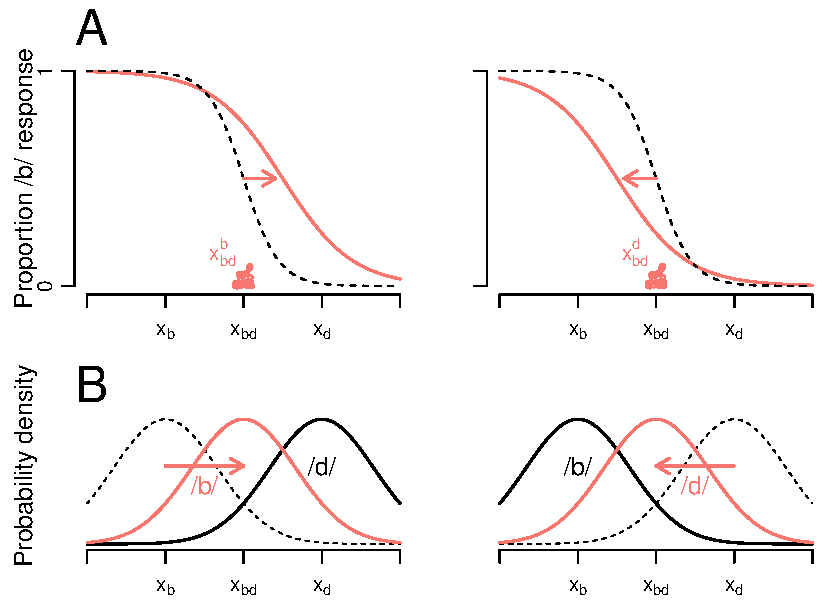
\includegraphics[width=0.75\textwidth]{figs/belief-updating-recal-schematic.pdf}
  \caption{Schematic illustration of the results of perceptual recalibration on classification of a \ph b-\ph d continuum (A), and the changes in the listener's beliefs about the underlying distributions which we propose to account for the changes in classification (B).  Dashed lines show pre-exposure classification functions and distributions, while solid lines show post-recalibration.  Left panels show the results of exposure to $x_\mathrm{bd}^\mathrm{b}$, and the right to $x_\mathrm{bd}^\mathrm{d}$.}
  \label{fig:belief-updating-schematic}
\end{figure}

Perceptual recalibration rapidly results in shifted category boundaries. For example, after as few as 10 exposures to $x_\mathrm{bd}^\mathrm{b}$, the /b/ category has `grown': more of the continuum is now classified as /b/, when tested without the labeling information \cite{Vroomen2007}. The opposite shift is observed for exposure to $x_\mathrm{bd}^\mathrm{d}$. This is illustrated schematically in Figure~\ref{fig:belief-updating-schematic} (A). Similarly rapid perceptual recalibration has been observed along a variety of phonetic contrasts, including vowels \cite{Maye2008a}, fricative place of articulation and manner \cite{Kraljic2005,Norris2003}, and stop consonant place \cite{Bertelson2003} and voicing \cite{Kraljic2006}.  Perceptual recalibration is typically investigated under the assumption that it reflects the same processes that support general accent adaptation.  This assumption is not trivial but there is some support that perceptual recalibration is not simply an artifact of the stimuli being presented in isolation \cite{Eisner2006} or there only being one unusual pronunciation \cite{Reinisch2014}.  We return to these issues in the next section. %Section~\ref{sec:recal-categ-shift}.

Qualitatively, perceptual recalibration exhibits several properties that are expected under the ideal adapter framework. First, recalibration seems to reflect implicit learning over phonetic contrasts, rather than strategic effects such as response bias \cite{Clarke-Davidson2008}, or weakening of the criterion for what counts as an acceptable example of a category \autocite[][but see next section]{Maye2008a}.
Recalibration also appears to affect speech perception through changes in sublexical phonetic category representations since perceptual recalibration effects generalize to novel words by the same talker containing the recalibrated segment \cite{McQueen2006}.

Second, perceptual recalibration seems to last: when listeners classify tokens from the same talker 12 hours after initial testing, the magnitude of adaptation is the same as right after initial exposure \cite{Eisner2006}. As we discuss in more detail in the second part of this article, longevity of changes in category boundaries (for a particular situation) is expected under our proposal that adaptation serves to make speech perception robust to changes in situation.

More specifically, the qualitative changes in classification boundaries observed during perceptual recalibration is naturally predicted by the ideal adapter framework (Figure~\ref{fig:belief-updating-schematic}, B).  Take, for example, the case where the listener is exposed to $x_\mathrm{bd}^\mathrm{b}$ (Figure~\ref{fig:belief-updating-schematic}, left).  As the listener updates their beliefs about the shifted distribution of cues for \ph b, shifting the mean towards the observed cue values, stimuli in the middle of the \ph b-\ph d continuum which previously had roughly equal likelihood under either category (and thus are sometimes perceived as \ph b and sometimes as \ph d) are now more likely to have resulted from \ph b, resulting in more \ph b responses to unlabeled test stimuli, especially in the previously-ambiguous region of the continuum.

\subsection{Incremental recalibration}
\label{sec:incr-recal}

It is encouraging that the ideal adapter framework provides a qualitative account of the results of recalibration.  But can this framework account for \emph{incremental} changes in behavior?  Belief updating is an incremental process, where the listener accumulates information about the talker's cue distributions one observation at a time.  The ideal adapter framework thus not only predicts asymptotic classification behavior---after the listener has fully adapted to the talker's cue distributions---but also how their classification behavior changes with each additional piece of evidence.
Unfortunately, few studies have investigated the \emph{incremental} effects of exposure to a novel distribution of sounds, such as would be typical for a new talkers.

A notable exception is \citeA{Vroomen2007}.  Listeners in their study were exposed to repetitions of an audio-visual adaptor, which was composed of a video recording of a talker articulating either \ph{aba} or \ph{ada}, dubbed with an audio item from a 9-item, synthetic \ph{aba} ($x_\mathrm{b}=1$) to \ph{ada} ($x_\mathrm{d}=9$) continuum.  The audio component for each participant was the continuum item that was most ambiguous, $x_\mathrm{bd}$.  The most ambiguous item was determined during a pre-test block of 98 trials where the entire \ph{aba}-\ph{ada} continuum was classified.\footnote{There were 14 repetitions of each stimulus, except for the two endpoints $x=1$ and $x=9$ which were repeated only 6 times and the next most prototypical items $x=2$ and $x=8$ which were repeated 8 times each}

Instead of the typical recalibration procedure, where exposure and test are separated, \citeA{Vroomen2007} measured the degree and direction of adaptation by interspersing audio-only test blocks throughout each exposure block, after 1, 2, 4, 8, 16, 32, 64, 128, and 256 cumulative exposures to the audio-visual adaptor.  Specifically, they measured the average proportion of \ph b responses to six-trial test blocks (the three most ambiguous items $\{x_\mathrm{bd}-1, x_\mathrm{bd}, x_\mathrm{bd}+1\}$ each repeated twice).

Each participant completed sixteen exposure blocks of 256 exposures.  Half of the exposure blocks used a \ph b audio-visual stimulus for exposure, and the other half used a \ph d.  Of the \ph b-exposure blocks, half of these used the auditorily ambiguous stimulus as described above, while the other half used the prototypical \ph b endpoint of the acoustic continuum ($x=1$), and likewise for the \ph d-exposure blocks.\footnote{The prototypical exposure blocks are discussed later.} %in Section~\ref{sec:selective-adapt}.}
Because our goal is to illustrate the workings of the ideal adapter framework when the listener has little prior experience that might be relevant for the current situation, we focus on the first 64 exposures of the first block from each participant (we return to the issue of extended exposure below).

\begin{figure}[htb]
  \centering
  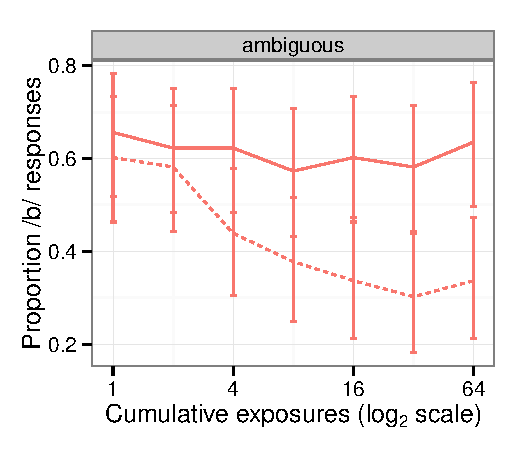
\includegraphics[width=0.5\textwidth]{vroomen-bd-recal-first-64.pdf}
  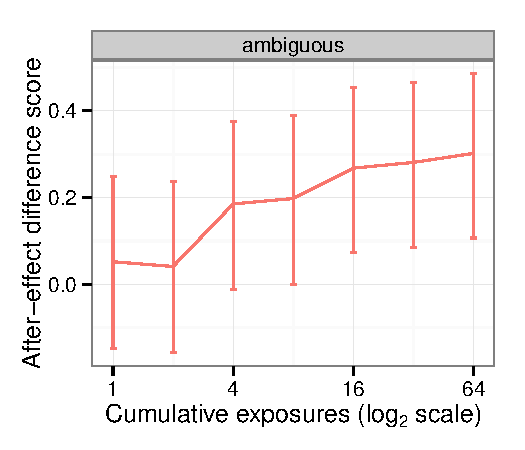
\includegraphics[width=0.5\textwidth]{vroomen-ae-recal-first-64.pdf}
  \caption{Recalibration results from Vroomen et al. (2007), showing both the proportion of \ph b responses (top, solid line \ph b exposure and dashed line \ph d exposure) and the aftereffect difference score (bottom) for the first 64 critical exposures in the first exposure block. Error bars indicate 95\% confidence intervals.}
  \label{fig:vroomen-results-64-recal}
\end{figure}

Figure~\ref{fig:vroomen-results-64-recal} shows the results of \citeA{Vroomen2007} demonstrating the build-up of recalibration in the first 64 critical exposures in the first exposure block.  The top panel shows the proportion \ph b responses for $x_\mathrm{bd}^\mathrm{b}$ and $x_\mathrm{bd}^\mathrm{d}$ adaptors separately; more \ph b responses after \ph b exposure (solid line) indicates recalibration, and vice-versa for \ph d exposure (dashed line).  A natural measure of the degree of recalibration is thus the \emph{aftereffect} difference score between \ph b and \ph d exposure.  A positive aftereffect indicates that \ph b exposure increased \ph b responses, and \ph d exposure \emph{decreased} \ph b responses (and increased \ph d responses), which corresponds to recalibration (Figure~\ref{fig:vroomen-results-64-recal}, bottom).

Recalibration builds up rapidly but incrementally over the first 64 exposures.  As discussed above, this build up follows naturally from the ideal adapter framework, as each exposure to the auditorily ambiguous adaptor contributes to a shift in the listener's estimate of the category mean.
Next, we quantify and test this prediction.


\subsection{Modeling build-up of recalibration}
\label{sec:modeling-build-up}

In order to evaluate the ability of the ideal adapter framework to account for the results of \citeA{Vroomen2007} on the incremental build-up of recalibration, we implemented a basic Bayesian belief updating model based on the principles of the ideal adapter framework.

\subsubsection{Bayesian belief updating model}
\label{sec:bayes-beli-updat}

We used a mixture of Gaussians as the underlying model of phonetic categories, where each phonetic category $c \in \{\mathrm b, \mathrm d\}$ corresponds to a normal distribution over cue values $x$ with mean $\mu_c$ and variance $\sigma^2_c$ (e.g. Figure~\ref{fig:dist-id-schematic}, top).  Thus, the likelihood of observation $x$ under category $c$ is
\begin{equation}
  \label{eq:4}
  p(x_i \given c, \boldsymbol{\mu, \sigma}^2) = \mathrm{Normal} (\mu_{c}, \sigma^2_{c})
\end{equation}

The listener's uncertain beliefs about phonetic categories are captured by additionally assigning probability distributions to the means $\mu_c$ and variances $\sigma^2_c$ of each phonetic category.  The prior distribution $p(\mu_c, \sigma^2_c)$ represents the listener's beliefs about category $c$ before exposure to the experimental stimuli, and the posterior $p(\mu_c, \sigma^2_c \given X)$ captures the listener's beliefs after exposure to stimuli $X = (x_1, x_2, \ldots, x_N)$ which are known to come from category $c$ (which means that the category labels $C=c$ are known).  These two distributions are related via Bayes' Rule:
\begin{equation}
  \label{eq:5}
  p(\mu_c, \sigma^2_c \given X, C=c) \propto p(X\given \mu_c, \sigma^2_c, C=c) p(\mu_c, \sigma^2_c)
\end{equation}

We used a conjugate prior for the Normal distribution with unknown mean and variance (Appendix~\ref{sec:model-fitting-methods}), and this prior distribution has two types of hyperparameters.\footnote{We use the term {\em hyperparameters} for terminological clarity to distinguish the \emph{model} parameters from the \emph{category} distribution parameters---means and variances---whose prior and posterior distributions are defined by the model parameters, the hyperparameters.}  The first set of hyperparameters captures the prior expected values of the means and variances.  The second set of hyperparameters captures the degree of confidence, or, conversely, uncertainty associated with the prior beliefs.  Put differently, they determine how much current observations are weighted against previous experience in determining beliefs about the category distributions.  In this model, there are two different degrees of confidence: one for the category means, denoted $\kappa_0$, and the other for the category variances, denoted $\nu_0$ (see the Appendix %~\ref{sec:model-fitting-methods}
for details).
An intuitive interpretation of these hyperparameters is as the effective sample size of the prior beliefs.  For instance, if the category mean confidence parameter is $\kappa_0 = 10$, then after ten \emph{new} observations the listener's beliefs about the category mean to equally reflect previous and current experience.  With fewer than ten new observations, the listener's beliefs about the category mean will be dominated by the mean expected based on previous experience; with more than ten new observations the beliefs about the mean will be increasingly dominated by the mean of the new observations.  These hyperparameters thus capture the gradient trade-off between prior experience and current experience in determining the listener's beliefs about phonetic categories.  They can be thought of as {\em pseudocounts} or the number of prior experiences that are relevant for the current situation.
\footnote{Even though comparable fits can be obtained using a single, overall effective prior sample sizes (e.g. $\kappa_0=\nu_0$), the two were fit as separate in order to evaluate the extent to which recalibration was primarily driven by a shift in the category mean or a change in variance.}

Finally, it is not a priori obvious whether adaptation occurs at the level of auditory cues individually or at some higher level where information is integrated from multiple auditory and/or visual cues.  Thus the model includes a third hyperparameter, $w$ which determines the weight given to the visual cue value in determining the percept.  This hyperparameter ranges from $w=0$ (perceived cue value is not influenced by the visual cue) and $w=1$ (perceived cue value entirely determined by the visual cue).  Adaptation over integrated cues might arise because the listener attempts to infer the talker's \emph{intended} production based on multiple partially informative cues \autocite[including top-down category distribution information,][]{Feldman2009a}.  For more discussion, refer to the Appendix. %Appendix~\ref{sec:audio-visual-cue}.

\subsubsection{Model fitting}
\label{sec:free-parameters}

The hyperparameters were fit in a two-step process, which is described in detail in the Appendix.  %~\ref{sec:model-fitting-methods}.
The first step is to fix the expected prior means and variances based on the classification curves measured during pre-test, before exposure to the audiovisual adaptor.  These hyperparameters are thus not free parameters of the model, in that they are not adjusted to improve the fit to the actual adaptation test data.

The second step is to estimate the three free hyperparameters (i.e., the effective prior sample sizes $\nu_0$ and $\kappa_0$ and the visual cue weight $w$) based on the actual adaptation data. The posterior distribution of the free hyperparameters was obtained using MCMC sampling with a weakly informative prior \autocite[to ensure a proper posterior,][]{Gelman2003}. For further details, we refer to Appendix~\ref{sec:model-fitting-methods}.
Because of the limited amount of data from each participant (only six trials per test block), we chose to fit the model to the aggregate data from all participants (see Appendix~\ref{sec:model-fitt-param} for motivation).

\subsection{Results and discussion}
\label{sec:results}

\begin{figure}[htb]
  \centering
  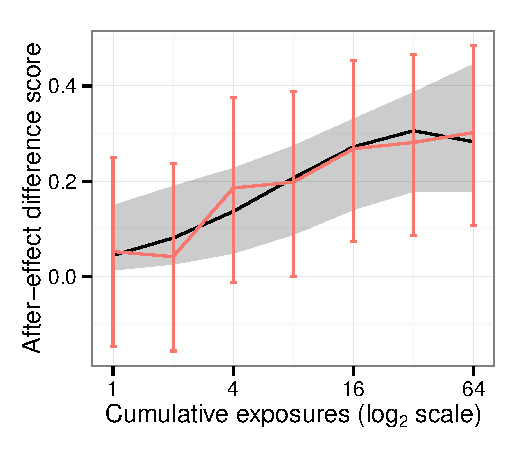
\includegraphics[width=0.5\textwidth]{figure/vroomen-recal-ae-fits-first-64.pdf}
  \caption{Belief updating model fit to build-up of recalibration data from Vroomen et al. (2007).  The $x$-axis shows the number of cumulative exposures to the adaptor (on a log scale), and the $y$-axis shows the aftereffect difference score.  The solid black line shows the MAP (maximum a posteriori) estimate predictions ($r^2=0.96$). The error bars and shaded region show 95\% credible intervals for the data and model predictions, respectively (see Appendix~\ref{sec:likel-test-stim}). }
  \label{fig:recal-buildup-preds}
\end{figure}

The model's fit against the data is shown in Figure~\ref{fig:recal-buildup-preds}. The predicted responses are plotted on the aftereffect scale for better comparison to \citeA{Vroomen2007}. The model effectively captures the qualitative fact that recalibration leads to positive aftereffects which  build up incrementally, and provides a quantitatively good fit as well ($r^2=0.96$).  Specifically, the model captures the fact that recalibration starts off relatively weak and gradually becomes stronger, before eventually leveling off.  Thus, not only is the qualitative result of recalibration---a positive aftereffect---predicted by the ideal adapter framework, the effect of cumulative exposure on the incremental build-up of the effect is also predicted well.  This suggests that listeners incrementally integrate each observed cue value with their prior beliefs in a way that is predicted by the ideal adapter framework.

We can draw a number of conclusions from the values of the hyperparameters themselves.
The best-fitting hyperparameter values are $\nu_0=71$, $\kappa_0=11$, and $w=0.53$.
First,
relative to the real overall sample size---the number of \ph bs and \ph ds encountered in the world by a typical English-speaking adult---the best-fitting effective prior sample sizes are \emph{extremely} low.
That is, listeners appear to put very little weight on their prior beliefs, adapting very quickly to the shifted cue distribution that they observe while taking slightly longer to adapt to the tight clustering (low variance).
This may be surprising at first glance, but it is actually qualitatively \emph{predicted} by the ideal adapter framework.
In the ideal adapter framework, whether or not (and how much) a listener adapts depends on how relevant they think their previous experiences are for the current situation. Thus in situations like a recalibration experiment where listeners encounter odd-sounding, often synthesized speech in a laboratory setting, they may have little confidence, a priori, that any of their previous experiences are directly informative. We discuss this point in length in the second half of this paper, where we elaborate on the crucial role of prior experiences for robust speech perception.

Second, the best-fitting value of the visual cue weight hyperparameter $w$ places approximately equal weight on the audio and visual cue values.  This means that, according to the best-fitting model, listeners perceive the cue value as not fully ambiguous. This makes an interesting prediction about the effects of extended exposure to the same stimulus that we return to below. %in Section~\ref{sec:effects-long-term}).

Third, the joint distribution---rather then just the point estimates---of the prior effective sample size hyperparameters (Figure~\ref{fig:vroomen-recal-joint-posterior}) reveal that as long as \emph{one} of these hyperparameters is low---on the same order of magnitude of the number of exposures to the adaptor stimulus---the other confidence hyperparameter can become extremely large and not change the model's predictions so much that the likelihood suffers.  This is because there are two ways that the positive aftereffect observed here (and in other recalibration studies) might come about after exposure to an ambiguous adaptor stimulus. This is discussed in more detail next.



\section{Recalibration by category shift or expansion?}
\label{sec:recal-categ-shift}

One of the advantages of model-fitting using Bayesian methods is that it allows us to evaluate the {\em range} of model hyperparameters which provide a good fit to the data. For the build-up of recalibration modeled in the previous section, the full posterior distribution over model hyperparameters (effective prior sample sizes and visual cue weight) provides interesting insight into how a human learner might adapt. To illustrate this, we examine the posterior distribution of the prior effective sample sizes for the category means and variances given the behavioral data.

\begin{figure}[htb]
  \centering
  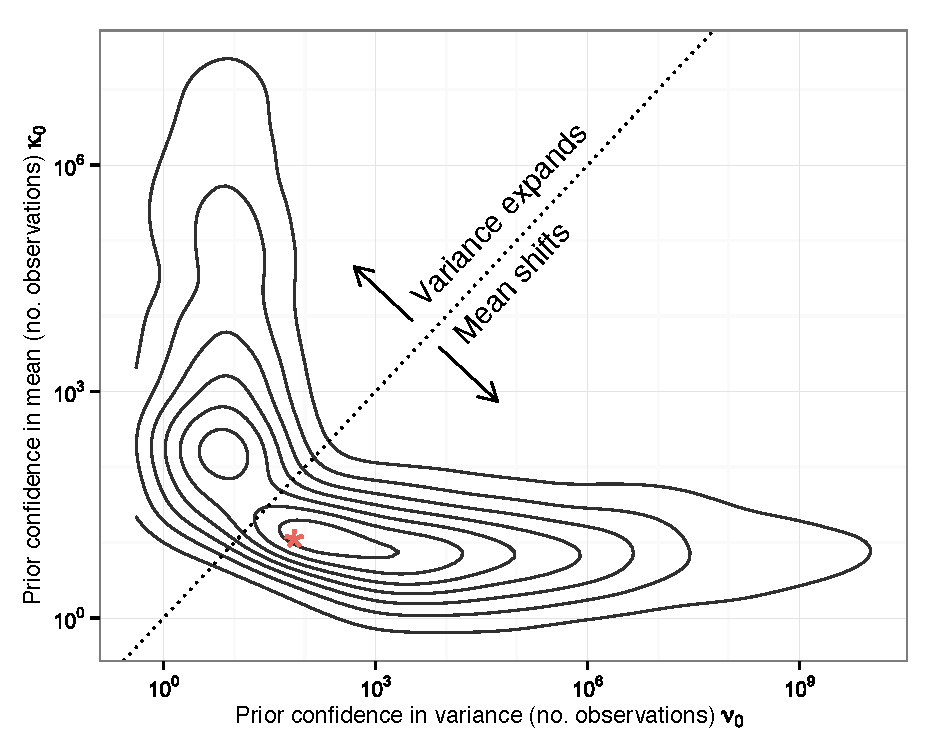
\includegraphics[width=0.8\textwidth]{figure/vroomen-recal-64-kappa-nu-joint-posterior-contour.pdf}
  \caption{The belief-updating model finds two different ways of fitting the build-up of recalibration (Figure~\ref{fig:recal-buildup-preds}), as illustrated by this density plot of the distribution of the mean and variance prior confidence parameters ($\kappa_0$ and $\nu_0$, respectively) that are consistent with the data (estimated by samples via MCMC).  The diagonal shows solutions with equal confidence in prior beliefs about the mean and variance.  Points below the line have higher confidence in the variance, and adapt by shifting the category mean.  Points above the line have higher confidence in the \emph{mean} and adapt by expanding the category variance.  Note that even though the best-fitting parameters (red asterisk, and curve in Figure \ref{fig:recal-buildup-preds}) are below the line (and shift the mean), there are areas of high posterior probability on both sides of the line (hills on the contour plot).} 
  \label{fig:vroomen-recal-joint-posterior}
\end{figure}

The joint distribution of the two confidence hyperparameters---the mean confidence $\kappa_0$ and the variance confidence $\nu_0$---is shown in Figure~\ref{fig:vroomen-recal-joint-posterior}.  This distribution covers an extremely wide range of both hyperparameters, although this entire range still results in qualitatively consistent \emph{predictions} about the aftereffect at each level of exposure (Figure~\ref{fig:recal-buildup-preds}).  The wide range covered by the posterior distribution of hyperparameters is due to the limited amount of data available to the model in this particular case. Note that this is not a problem. It merely reflects that these data do not uniquely constrain the model. A human learner exposed to the same data would face the same problem. Indeed, we will see below that when the model is constrained by further data, the posterior distribution of the hyperparameters will become more narrow.

Of interest is that the posterior is bimodal: there are two ways that belief updating can account for the build-up of recalibration.  The best-fitting (MAP-estimate) hyperparameters correspond to a shift in the mean of the adapted category: the prior effective sample size of the mean, $\kappa_0$, is less than that of the variance, $\nu_0$, and as a result the prior beliefs about the mean are overcome more quickly than the variance.
However, this pattern is only true for roughly half the samples from the joint posterior of the hyperparameters ($p_\mathrm{MCMC}(\nu_0 > \kappa_0) = 0.55$).  In the other half of the samples, the prior effective sample size for the mean is on average very high, meaning that the positive aftereffect observed in the data is modeled as a change in the \emph{variance} of the adapted category, with a mean that is essentially fixed.

This combination of hyperparameters---flexible variance and fixed mean---can lead to a positive aftereffect after exposure to auditorily ambiguous but labeled tokens in the following way.  If the listener has very high confidence in the mean of each category coming into a new situation, then repeated exposure to an ambiguous segment which is labeled as belonging to one category is best explained by the hypothesis that the talker is producing that category with a high degree of variability.  Increasing the variance of the recalibrated category in this way means that more likelihood is assigned by that category to the previously-ambiguous part of the continuum to the recalibrated category, and thus leads to a positive aftereffect.

Thus, a positive aftereffect is qualitatively consistent with both a shift in mean \emph{and} an increase in category variance.  Moreover, the joint distribution of hyperparameters fit to the build-up of recalibration observed by \citeA{Vroomen2007} show that in the ideal adapter framework, the quantitative effect of cumulative exposure on the build-up of recalibration is also ambiguous in the same way.

\citeA{Maye2008a} behaviorally investigated a similar question.  Specifically, they wondered whether positive aftereffects typically observed in recalibration experiments were really due to a shift in the underlying category, or just a relaxation of the criterion for what counts as a good exemplar of the adapted category.  They exposed listeners to vowels that were shifted in a particular direction (e.g. shifting the high vowel \ph I in \emph{wicked} down to the mid vowel \ph E to make \emph{`wecked'}).  In a lexical decision task after exposure to such downward shifts, listeners accepted more nonwords that were downward-shifted versions of real words, but not nonwords that were upward-shifted words.  This corresponds, in the ideal adapter framework, to a shift in the means of the adapted categories, without a substantial change in the variance.

It may be tempting to conclude based on these results that \emph{all} recalibration effects result from shifting category means.  However, the ideal adapter framework predicts that positive aftereffects due to changes in \emph{either} means and variances are possible, in different situations, especially depending on whether the listener has greater confidence in their prior beliefs about category variances or means. This is, to the best of our knowledge, a novel prediction. Since one of our goals is to provide a guiding framework for future work on speech processing and adaptation, we elaborate on this prediction.

When might the listener have greater confidence in the mean of a category rather than its variance, and vice versa?  
In the ideal adapter framework, the listener's prior beliefs about a category parameter constitute a prediction about the distribution of values they might expect that parameter to take on in the future.  The level of confidence in prior beliefs is closely related to the level of variability of a particular category parameter that the listener expects across situations.  For cues whose typical values vary across situations (e.g. formant frequencies), an ideal adapter should expect substantial variability in the underlying means, in order to be prepared to shift their beliefs about category means on that cue when appropriate.

The variance of a particular cue for a particular category is closely related to how reliable that cue is at distinguishing one category from another \cite{Allen2004,Clayards2008,Newman2001,Toscano2010}: for two categories with fixed means, increasing the variance of both categories means that their distributions will overlap more and, on average, observing that particular cue will be less informative about the intended category.  Thus for a cue which varies in reliability from one situation to the next (with relatively stable category means), the ideal adapter should in general be more likely to adjust category variance than means.\footnote{This is not to say that an ideal adapter would \emph{not} adapt to changes in category distributions for cues whose means or variances do \emph{not} vary much across situations.
Rather, the amount of variability in a particular category's statistics over situations combines with the listener's overall level of confidence that their prior experience is relevant for the current situation.}

Thus, the ideal adapter framework predicts that there are range of strategies available to the listener for adapting to new talkers.  In real-life accent adaptation, there are usually \emph{many} categories and cue dimensions where an accent is unusual, and in some cases these differences can be due to both changes in the cue values typically used to realize a category (the mean) and changes in how reliable a given cue is at distinguishing a category (the variance).  In real speech there are many partially informative cues to any given category, and it may be a completely reasonable strategy for the listener to simply decide that a particular cue is uninformative and ignore it (or at least downweight it).

This points to a critical empirical gap in our understanding of speech perception. Most existing work on phonetic adaptation follows one of two approaches. The first approach emphasizes relatively natural conditions and accent variability, where language occurs in context (e.g. sentences) and listeners must adapt to accents that vary along many categories and cue dimensions \cite{Baese-berk2013,Bradlow2008,Clarke2004,Sidaras2009}.  The second approach is that of perceptual recalibration/learning, which typically presents speech as isolated words or syllables and emphasizes acoustic manipulation of a single category or auditory cue.  While perceptual recalibration has been observed when these unusual pronunciations were presented as part of running speech in a story \cite{Eisner2006} or as words spoken by a talker who has a real foreign accent \cite{Reinisch2014}, it is an open question under what conditions listeners downweight cues and when they track changes in mean cue values during naturalistic accent adaptation.

In order to address listeners' ability to adapt to novel talkers based on the statistical properties of their speech as predicted by the ideal adapter framework, we see two potentially fruitful directions.  First, we think that perceptual recalibration paradigms should be scaled up to explore the role of natural levels of within-category, within-talker variability and the role of controlled deviation in multiple categories and cue dimensions in recalibration.  Second, we think that naturalistic accent adaptation paradigms might be refined to specifically investigate how accent difficulty is driven by deviations---from unaccented speech---in the \emph{average} value of a cue versus unusual \emph{variability} in that cue.  Given that, across talkers, the average value of some cues varies quite a bit \cite{Newman2001}, while for others it is relatively consistent \cite{Allen2003}, it might be expected that listeners will have a harder time adapting to accented speech which is characterized by deviant values of cues that are typically stable across talkers \cite<like VOT>{Sumner2011}.

We have discussed how phonetic recalibration is qualitatively predicted by the ideal adapter framework, and presented a model in this framework which captures the incremental build-up of recalibration quantitatively.  In the next three sections we show how this framework provides a potentially unifying perspective on phonetic adaptation more broadly.



\section{Beyond recalibration: selective adaptation}
\label{sec:selective-adapt}


Next we apply the ideal adapter framework to a phenomenon known as selective adaptation \cite{Eimas1973,Samuel1986}.  Traditionally, selective adaptation is thought to be due to mechanisms that are distinct from those underlying perceptual recalibration.  We will show, however, that the cumulative build-up of selective adaptation is captured by the same belief-updating model introduced in the previous sections.

Selective adaptation occurs after repeated exposure to a single phonetic category, and is characterized by a \emph{negative} aftereffect, where fewer items on a phonetic continuum are classified as the adapted category.  For instance, and as we will discuss in more detail below, \citeA{Vroomen2007} found that repeated exposure to a \emph{prototypical} \ph b audio-visual adaptor constructed from the \ph b endpoint of their \ph b-\ph d continuum (rather than the ambiguous midpoint) resulted in \emph{fewer} \ph b responses during test trials (and vice-versa for \ph d).

Selective adaptation is broadly considered to be the result of either habituation of ``feature detectors'' which are sensitive to linguistically-relevant features of the acoustic speech signal, or contrast effects at a categorical level \cite{Samuel1986}.  It is also generally acknowledged that selective adaptation operates at a range of different levels.  On the one hand, non-speech phonetic analogues (like isolated F2 and F3 formant transitions) can selectively adapt a place of articulation contrast, which suggests that selective adaptation operates on relatively low-level auditory processing \cite{Samuel1996}. On the other hand, selective adaptation has also been shown to generalize between acoustically different but phonetically similar continua, suggesting that it does not depend solely on acoustic overlap \cite{Samuel1996,Sawusch1977}.

\subsection{Incremental selective adaptation}
\label{sec:incr-select-adapt}

\begin{figure}[htb]
  \centering
  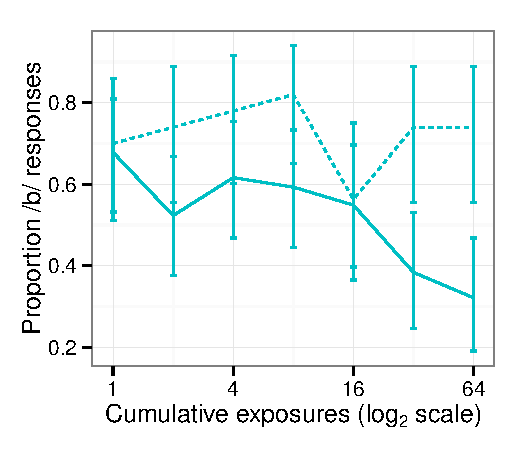
\includegraphics[width=0.5\textwidth]{vroomen-bd-selad-first-64.pdf}
  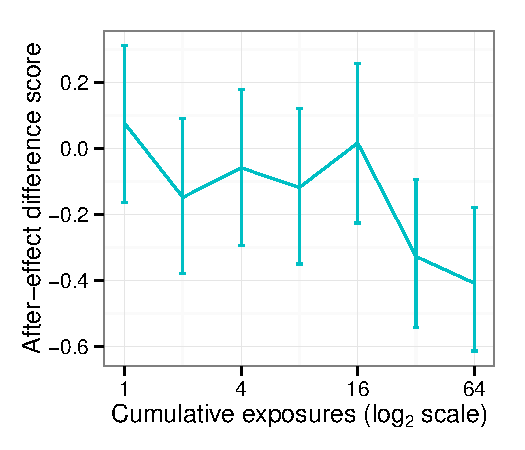
\includegraphics[width=0.5\textwidth]{vroomen-ae-selad-first-64.pdf}
  \caption{Selective adaptation results from Vroomen et al. (2007), showing both the proportion of \ph b responses (top) and the aftereffect difference score (bottom) for the first 64 cumulative exposures in the first exposure block. Error bars indicate 95\% confidence intervals.}
  \label{fig:vroomen-results-64-selad}
\end{figure}

As is the case with recalibration, there is little work on how selective adaptation builds up incrementally.  Again, one notable exception is \citeA{Vroomen2007}, who also investigated the build-up of selective adaptation at varying levels of exposure.  Selective adaptation was induced by repeated exposure to a prototypical audio-visual adaptor, made using the same video as the ambiguous audio visual stimuli from the recalibration conditions paired with the corresponding category endpoint ($x=1$ for \ph b and $x=9$ for \ph d).  Other than this, the design and procedure was exactly the same as the recalibration condition described above: listeners heard a total of 256 repetitions of one of these adaptors, and were tested on the same audio-only classification test after 1, 2, 4, 8, 16, 32, 64, 128, and 256 cumulative adaptor exposures.

Figure~\ref{fig:vroomen-results-64-selad} shows the results for the first 64 cumulative exposures in the first exposure block for selective adaptation from \citeA{Vroomen2007}.  Like with the recalibration conditions, selective adaptation builds up incrementally over the first 64 exposures (although there is quite a bit of noise due to the small number of observations).  Can a belief updating model account for this data?

\begin{figure}[htb]
  \centering
  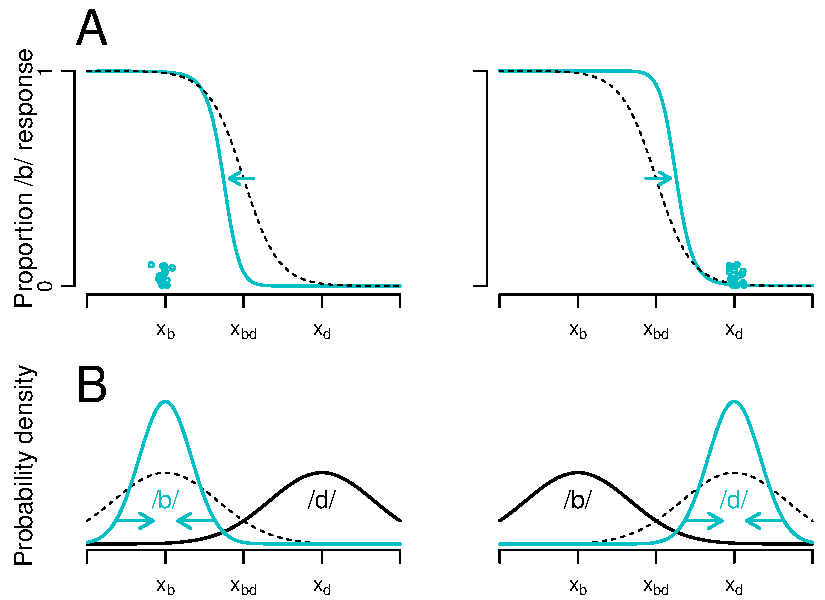
\includegraphics[width=0.75\textwidth]{figs/belief-updating-selad-schematic.pdf}
  \caption{Schematic illustration of the results of selective adaptation on classification of a \ph b-\ph d continuum (A), and the changes in the listener's beliefs about the underlying distributions which we propose to account for the changes in classification (B).  Dashed lines show pre-exposure classification functions and distributions, while solid lines show post-recalibration.  Left panels show the results of exposure to prototypical $x_\mathrm{b}^\mathrm{b}$, and the right to $x_\mathrm{d}^\mathrm{d}$.}
  \label{fig:belief-updating-selad-schematic}
\end{figure}


Qualitatively, the answer is yes, as shown schematically in Figure~\ref{fig:belief-updating-selad-schematic}.  Just like the recalibration condition, the distribution of cues that listeners encounter in the selective adaptation condition is unusual: the exact same cue value is repeated over and over again.\footnote{There is of course additional perceptual uncertainty or noise variance \cite{Feldman2009a}, but the combined variance from sensory uncertainty and actual stimulus variance across trials is still less for an identical repeated stimulus than would be expected with normal levels of variability.}  In natural speech there is inevitable variability in the cue values used to realize a single phonetic category, and thus the level of consistency in this experiment is highly unusual.  A belief updating model predicts that listeners will adjust their beliefs about the variance of the adapted category as a result of these unusual statistics.  The results of adapting to low-variance exposure to, e.g., a prototypical \ph b is that the \ph b category `shrinks', and cues values that were previously ambiguous become less likely under \ph b and thus more likely to be classified as \ph d (Figure~\ref{fig:belief-updating-selad-schematic}, top).  This is the negative aftereffect that characterizes selective adaptation.

While few studies have investigated the effect of unusual category variance on subsequent perception, one notable exception is \citeA{Clayards2008}.  They showed that listeners who are exposed to \ph b and \ph p sounds whose VOTs have low variance show a sharper category boundary than listeners exposed to high variance distributions.  Moreover, the difference in category boundary slopes is exactly as predicted by the category variances, via an ideal listener model.  This suggests that listeners adjust their categorization behavior based on recently experienced within-category \emph{variance} of acoustic cues, exactly as the ideal adapter framework predicts.

\subsection{Modeling the build-up of selective adaptation}
\label{sec:methods-results}

The ideal adapter framework---and the model introduced above---makes further predictions about how classification behavior depends on the \emph{amount} of exposure, as well as its statistical properties.  In order to evaluate the ability of belief updating to quantitatively account for the build up of selective adaptation, we fit the same model that was fit to the recalibration data above to the first 64 exposures of the selective adaptation data from the first block of each participant in \citeA{Vroomen2007}.

\subsection{Results}
\label{sec:results-discussion}

\begin{figure}[htb]
  \centering
  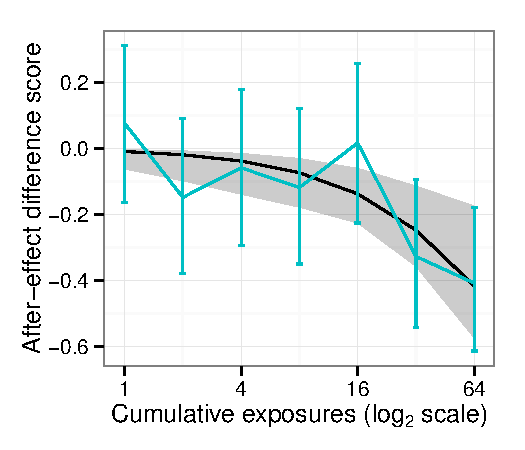
\includegraphics[width=0.5\textwidth]{figure/vroomen-selad-ae-fits-first-64.pdf}
  \caption{Belief-updating model fits to the data from Vroomen et al. (2007) on the build up of selective adaptation after varying levels of cumulative exposure to a prototypical audio-visual adaptor ($x$-axis, on a log scale).  The solid black line shows the MAP (maximum a posteriori) estimate predictions ($r^2=0.83$). The error bars and shaded region show 95\% credible intervals for the data and model predictions, respectively. }
  \label{fig:selad-buildup-preds}
\end{figure}

The model also fits the selective adaptation data well ($r^2=0.83$), as shown in Figure~\ref{fig:selad-buildup-preds}.  As the model predicts, selective adaptation starts very weakly, gradually becoming stronger with further exposure.  The build-up of selective adaptation also appears to accelerate, unlike recalibration, with further exposure producing even larger increases in the strength of the selective adaptation effect, which is also captured by the model.  Thus, while selective adaptation is not usually considered the result of belief updating or distributional learning, the same belief updating model which describes well how listeners integrate each observation with their prior beliefs during recalibration \emph{also} describes the build-up of selective adaptation.

The best-fitting (MAP estimate) hyperparameters for the selective adaptation data are also nearly identical to the recalibration estimates: the effective prior sample size for the variances is $\nu_0=64$ (vs. 71), and for the means, $\kappa_0=13$ (vs. 11).  The visual cue weight is $w=0.51$ (vs. 0.53).  This demonstrates two points.  First, as with recalibration, these values correspond to very small effective prior sample sizes, which suggests that listeners do not believe that their vast amount of prior experience with \ph bs and \ph ds is very relevant in this situation.

Second, even though these parameter values correspond to higher prior confidence in the variance than the mean, the model nevertheless accounts for selective adaptation via shrinking category variance.  This is because, unlike the ambiguous adaptor, for the prototypical adaptor there is no difference between the observed and expected category means.  In this case, the updated estimate of the variance is simply an average of the prior expected and the observed variance, weighted by the effective prior sample size and actual sample size, respectively (see Appendix~\ref{sec:belief-updating-with}, Equation~\eqref{eq:post-sum-of-squares}).  For the best-fitting estimate of the effective prior sample size $\nu_0=64$ and an observed variance of zero, this means that the model believes the category variance to have halved after 64 exposures.

\subsection{Discussion}
\label{sec:discussion-sel-ad}

These results suggest that, at least for the classification results of \citeA{Vroomen2007}, it is not necessary to invoke a qualitatively distinct process to explain selective adaptation. The ideal adapter also makes the correct qualitative predictions for a variety of other selective adaptation experiments \autocite[e.g.,][]{Eimas1973,Miller1983}.  It might thus be tempting to assume that {\em all} selective adaptation effects can be reduced to distributional learning of the type proposed here. Such an account will face several serious challenges. This includes the need to account for complex reaction time effects induced by different types of selective adaptation \cite{Samuel1986,Samuel1996}, about which our ideal adapter framework does not yet have anything principled to say. Rather than discuss this and other challenges to an ideal adapter account of selective adaptation here, we merely note that much work remains to be done in fleshing out the predictions of the ideal adapter framework for selective adaptation more generally.

\label{r4-zerovar}
In particular, three directions for future work stand out.  First, in order to link the ideal adapter framework to reaction time data, process models have to be developed. Second, our account of selective adaptation depends on the listener's \emph{perceived} variance of each distribution, which may not be the same as the measured variance of some physical cue.  We have made the simplifying assumption here that the perceived variance is the same as the actual variance.  For extreme cases, like the case of selective adaptation studied here, where there is \emph{no} (or minimal) variance in the physical signal, this assumption leads to implausible asymptotic behavior: with more and more exposure, the category should shrink to nothing, leading to an asymptotic aftereffect of $-1$.  Of course, between 128 and 256 exposures, the negative aftereffect induced by selective adaptation appears to continue to grow stronger (Figure~\ref{fig:vroomen-results-64-selad}), suggesting that it has not yet reached its actual asymptote, but we do not know what that is for this paradigm.  The distinction between perceived and actual variance becomes even more important when making quantitative predictions about different levels of variance.  If the sensory uncertainty (or noisiness in the perceptual system) contributes substantially to the perceived variance \autocite[for preliminary evidence, see][]{Clayards2008,Feldman2009a,Kronrod2012}, this is expected to reduce or eliminate predicted effects of variation in physical variance.

\label{r4-sensory-adapt}
Third, our account opens the door to alternative interpretations of particularly challenging aspects of listeners' classification behavior after selective adaptation \cite{KleinschmidtInPrep}. More generally, recent work on non-linguistic sensory adaptation (mostly in low-level vision and audition) has revealed that many negative aftereffects which were originally attributed to the fatigue of neuronal feature detectors are better explained by neural populations adjusting their processing to maximize the transmission of information about the current stimulus ensemble \cite{Brenner2000,Fairhall2001,Gutfreund2012,Kohn2007,Sharpee2006,Webster2005}, which parallels recent developments in the understanding of perceptual learning in low-level perceptual tasks \cite{Bejjanki2011a,Harris2012}.  Maximizing information transmission depends on the statistics of the environment at many different levels.

For speech perception, sometimes the relevant statistics are at the level of the phonetic generative model---the cue distributions for each category---but sometimes they are at a different level, such as the distributions of categories themselves or the spectral characteristics of background noise which must be ignored.  For instance, \citeA{Huang2012} found that the classification boundary between ``bet'' and ``but'' could be manipulated simply by preceding exposure to a pure tone: when the frequency was near the second formant frequency of ``bet'', listeners made fewer ``bet'' responses.  This seems incompatible with the idea that selective adaptation is due to the listener updating their beliefs about the distribution of cues associated with a particular category, but it is entirely consistent with a more general view that adaptation reflects changes in the listener's beliefs about which cues are more likely to occur---or be behaviorally relevant---across different levels of processing.  That is, even though selective adaptation may not always represent updating beliefs about the talker's generative model, it may still serve the same purpose: efficient processing of linguistically-relevant acoustic signals in a world where the statistical properties of those signals vary across situations \cite{KleinschmidtInPrep}.  However, straightforward application of a model like the one presented here to perceptual inference at lower levels has not been successful \cite{Stocker2006} and more work remains to flesh out this connection.

\label{r1-computation-mechanism}
For the current purpose, it is sufficient to conclude that not everything that looks like selective adaptation requires an explanation in terms of a separate computation.
Despite the fact that recalibration and selective adaptation are typically considered to be qualitatively distinct phenomena, we have shown that a single belief updating model  can account for the early, incremental build-up of both of these effects.  This is achieved under essentially identical assumptions about prior effective sample sizes and the audio-visual cue weight (the hyperparameters in our model).  We have also shown that the process of the listener updating their beliefs about category variance provides a likely explanation for at least some adaptive behaviors during speech processing \autocite[see also][]{Clayards2008}.
In the next section, we explore the consequences of this shrinking category variance in response to a repeated adaptor stimulus for prolonged exposure to a repeated stimulus.



\section{Effects of prolonged repeated exposure to the same stimulus}
\label{sec:effects-long-term}


The ideal adapter framework predicts that when presented with a single, repeated stimulus, the listener should shrink the variance of the repeated category.  This leads to predictions about the incremental effects of selective adaptation by a prototypical sound (discussed in the previous section), but it also makes an interesting prediction about repeated exposure to an \emph{ambiguous} sound.  Even though listeners typically do not encounter a physically identical sound repeatedly in real life, the use of repeated sounds is common in perceptual recalibration experiments, which often use a single repeated token \autocite[e.g.,][]{Bertelson2003,Vroomen2004} or multiple words where the critical segment is replaced with the same ambiguous sound \autocites[e.g.,][]{Norris2003,Samuel2001}[but see][]{Kraljic2005,Reinisch2014}.

Recall that according to the belief-updating model presented above, in the recalibration condition of \citeA{Vroomen2007} listeners do not perceive the adaptor cue value as fully ambiguous.  Rather, their perceived cue value combines the ambiguous acoustic cue value and the prototypical visual cue value with roughly equal weight (visual cue weight parameter $w=0.53$).  The belief-updating model predicts that with repeated exposure to this not-quite-ambiguous adaptor, after the shift in the mean to the observed cue value, the low observed variance will eventually lead to the category shrinking and pulling back from the middle of the continuum. This prediction is illustrated in Figure~\ref{fig:mcgurk-preds-schematic}.

\begin{figure}[htb]
  \centering
  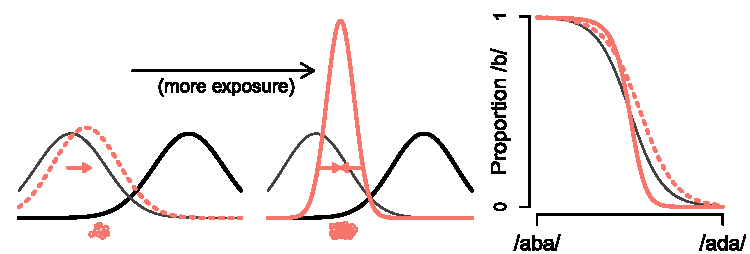
\includegraphics[width=\textwidth]{schematic-recal.pdf}
  \caption{Schematic illustration of the predicted trade-off between shifts in mean and change in variance.  With exposure to tightly clustered (or repeated) stimuli which are perceived as not fully ambiguous, the ideal adapter predicts that the initial shift in mean should lead to a positive aftereffect with small amounts of exposure (left, and dashed line), while the low variance of the repeated adaptor eventually leads to a neutral or even negative aftereffect with prolonged exposure (middle).}
  \label{fig:mcgurk-preds-schematic}
\end{figure}

This results in an eventual \emph{decrease} in the likelihood that the adapted category assigns to the auditorily ambiguous test stimuli in the middle of the continuum and predicts that the positive after-effect associated with recalibration will eventually weaken and possibly even reverse if the category pulls back far enough.  We have seen a hint that this may in fact occur: recalibration seems to effectively level off by 64 cumulative exposures in the data from \citeA{Vroomen2007}.  In this section, we further test this prediction by looking at the additional data that \citeA{Vroomen2007} collected for up to 256 cumulative exposures.


\begin{figure}[htb]
  \centering
  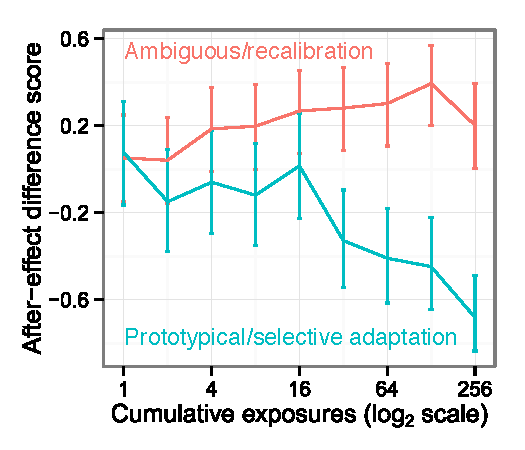
\includegraphics[width=0.5\textwidth]{vroomen-ae-first.pdf}
  \caption{Results from Vroomen et al. (2007), showing the full 256 exposures.  Red/top curve: ambiguous audio-visual adaptor (recalibration).  Blue/bottom curve: prototypical audio-visual adaptor (selective adaptation).}
  \label{fig:vroomen-results-256}
\end{figure}

\subsection{Data}
As discussed above, \citeA{Vroomen2007} exposed listeners to a total of 256 repetitions of the audiovisual adaptor.  Figure~\ref{fig:vroomen-results-256} shows the results from both conditions, including the test trials at 128 and 256 cumulative exposures.  As qualitatively predicted, the negative aftereffect associated with selective adaptation grows stronger with further exposure, while the positive aftereffect associated with recalibration plateaus and even begin to decline after 256 exposures.\footnote{While the decline in recalibration appears to be relatively modest in the figure here, Vroomen et al. (2007) actually found much stronger declines in recalibration in their full data set, where recalibration essentially disappears by 256 exposures.  Our replication presented in the next section establishes that such a decline can occur in the first block (Figure~\ref{fig:intr-results-fits}), suggesting that the failure to observe it strongly in the first block of Vroomen et al. (2007) is due to individual differences, which are substantial.}

\begin{figure}[htb]
  \centering
  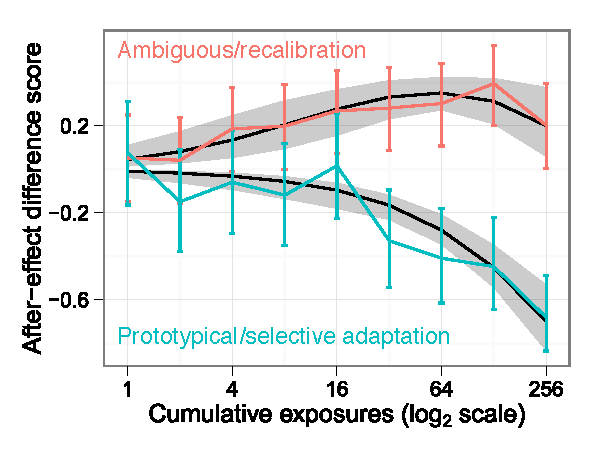
\includegraphics[width=0.5\textwidth]{vroomen-preds-firstblock.pdf}
  \caption{Results from fitting the belief updating model to all 256 exposures in both conditions from Vroomen et al. (2007) simultaneously.  Model predictions correspond to MAP-estimate hyperparameters of $\nu_0 = 100$, $\kappa_0=17$, and $w=0.47$.}
  \label{fig:model-fits-vroomen-256-simult}
\end{figure}

\subsection{Results and discussion}
To quantify these predictions and test whether the belief updating model can account for the decrease in recalibration, we fit it to the data from all 256 exposures to the ambiguous and prototypical adaptors.
The model fits well when fit to either the ambiguous or prototypical conditions individually ($r^2=0.86$ in both cases). To further test the model's ability to provide a unified explanation of recalibration and selective adaptation, we fit the model to both conditions simultaneously.

Figure~\ref{fig:model-fits-vroomen-256-simult} shows that the model simultaneously fits the behavioral data in both conditions quite well ($r^2=0.93$ overall, and $r^2=0.86$ and $0.85$ for the ambiguous and prototypical subsets, respectively).  There is no loss of goodness-of-fit from fitting both conditions simultaneously.  The best fitting hyperparameters were $\nu_0 = 100$, $\kappa_0=17$, and $w=0.47$.  These hyperparameters are very similar to the best-fitting hyperparameters for the first 64 exposures only, as well as the estimates when each condition is fit separately.

In particular, the best fitting models for the initial build-up (first 64 exposures) and prolonged exposure (256 exposures) place roughly the same weight on the visual cue ($w=0.53$ vs. $w=0.47$, respectively, where $w$ could range from 0 to 1), even though the decay in recalibration is virtually absent during the first 64 exposures. That is, just based on the rate at which recalibration initially accumulates, the model predicts the later decay without further assumptions.


\section{Exploring the predictive power of the ideal adapter}
\label{sec:expl-pred-power}

One of the benefits of a model like we present here is that it makes quantitative predictions which go beyond existing data.  In this section, we explore the ideal adapter framework's predictive power.  The fact that the ambiguous and prototypical conditions from \citeA{Vroomen2007} can be accounted for by a single set of belief updating model hyperparameters suggests that the recalibration and selective adaptation effects in this experiment are not qualitatively distinct but rather endpoints on a continuum of adaptation effects.  The ideal adapter framework predicts that for observed cues which are less ambiguous, the low variance of the adaptor distribution will be detectable with fewer observations, causing an earlier (and lower) peak in the positive aftereffect detected in the recalibration condition.


In order to test this prediction, we replicate and extend the design of \citeA{Vroomen2007}, adding intermediate conditions where the acoustic component of the audio-visual adaptor is neither fully ambiguous nor fully prototypical, but somewhere in between.  As a strong test of the predictive power of the model, we ask whether hyperparameters fit to the ambiguous/recalibration and prototypical/selective adaptation conditions in our replication can be used to predict adaptation behavior in new situations which have not been studied before.

\subsection{Methods}
\label{sec:methods-4}

We developed a novel web-based paradigm to efficiently collect phonetic categorization data from a large number of participants, adhering as closely as possible to the methods of \citeA{Vroomen2007}.  In addition to the ambiguous and prototypical conditions of \citeA{Vroomen2007}, we added two intermediate conditions: intermediate-ambiguous, and intermediate-prototypical.

\subsubsection{Stimuli}
\label{sec:stimuli}

Stimuli were identical to those used by \citeA{Vroomen2007}, who generously shared their materials.  The audio stimuli were items from a nine-item synthetic \ph{aba}-\ph{ada} continuum, created by shifting F2 locus in equal mel steps from a prototypical \ph{aba} value to a prototypical \ph{ada} value, holding other parameters constant \cite{Vroomen2004}.  The visual stimuli were natural videos of a male talker articulating \ph {aba} and \ph{ada}.

Audio-visual adaptors for the ambiguous and prototypical conditions were constructed as in \citeA{Vroomen2007}, by matching the video with the participant's most ambiguous continuum item $x_\mathrm{bd}$ or the corresponding continuum endpoint, respectively.  For the two intermediate conditions, the audio component was offset by one (intermediate-ambiguous) or two (intermediate-prototypical) positions towards the video category endpoint (Figure~\ref{fig:conditions-schematic}).

\begin{figure}[htb]
  \centering
  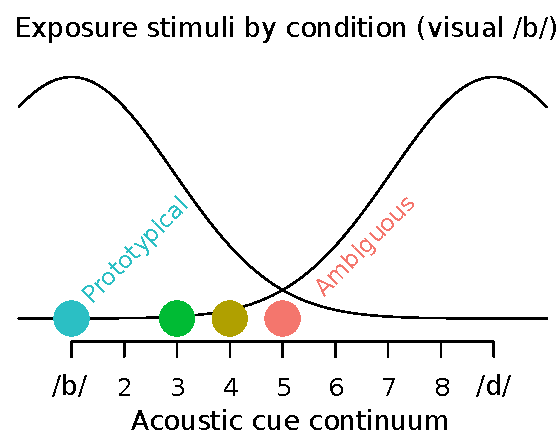
\includegraphics[width=0.5\textwidth]{figs/schematic-conditions-modified.pdf}
  \caption{Construction of stimuli for four conditions with visual \ph b (visual \ph d is analogously the mirror image).}
  \label{fig:conditions-schematic}
\end{figure}

\subsubsection{Procedure}
\label{sec:procedure}

Participants first performed the same pre-test \ph b-\ph d classification task as in \citeA{Vroomen2007} (described above).
After the calibration phase, participants were split into four exposure conditions (Figure~\ref{fig:conditions-schematic}): ambiguous and prototypical conditions as in \citeA{Vroomen2007}, plus two intermediate conditions. For the intermediate-ambiguous condition, the adaptors were constructed from the continuum item one position over from the most ambiguous position, in the direction of the endpoint corresponding to the video category.  The intermediate-prototypical adaptors were constructed from the continuum item two positions over from the most ambiguous item.  Each participant did two exposure blocks, one \ph b and one \ph d.

Each block consisted of a total of 128 audio-visual exposure trials.  Audio-only \ph b-\ph d test trials were interspersed after 1, 2, 4, 8, 16, 32, 64, 96, and 128 cumulative exposures, in blocks of 6 or 12 trials (2 or 4 repetitions of each participant's 3 most ambiguous stimuli).  Following the first exposure block, participants took a short break and completed the second block, with an audio-visual exposure stimulus from the opposite category but same condition.

The experiment was conducted over the web, via Amazon's Mechanical Turk crowd-sourcing service using a custom Javascript application.\footnote{This source code and a working demo are available from \url{http://hlplab.wordpress.com/2013/09/22/phonetics-online/}}  Response keys and block order were counter-balanced across participants.  The experiment took no longer than 45 minutes to complete.

\subsubsection{Participants}
\label{sec:participants}

A total of 280 participants were recruited.  Since participants were being run remotely, using a variety of audio equipment to complete the experiment, a number of quality checks were required.  First, our task was only made available to workers whose location was listed as the US and had more than 95\% of their previous work accepted for payment (an automatic quality control measure offered by Amazon).  Second, based on the calibration task, participants with unusual category boundaries \autocite[most ambiguous stimulus not one of the middle three positions 4, 5, or 6 found by][]{Vroomen2007} were automatically excluded from the remainder of the experiment.  60 participants were excluded for this reason.  Third, participants who classified the two endpoint stimuli and their nearest neighbors ($x=1,2,8,\textrm{ or } 9$) with less than 70\% accuracy were also excluded.  25 additional participants were excluded for this reason.

Fourth, in order to ensure that participants were actually watching the videos during the exposure phase, catch trials were interspersed throughout exposure \autocite[as in][]{Vroomen2007}.  These trials were identical to normal audio-visual exposure trials, except for a small white dot which flashed for one frame above the talker's lip.  On these trials, participants were instructed to press the space bar to indicate they saw the dot.  Participants who missed more than a total of 20\% or more than 50\% on any one block were excluded from analysis and replaced (13 participants).  After this exclusion, the overall catch trial accuracy rate was 96\% \autocite[compared to 93\% reported by][]{Vroomen2007}.

Following good statistical procedure \cite{Simmons2011}, these exclusion criteria were fixed before beginning data collection and automatically executed by our experiment software.
Data from a total of 182 participants remained for analysis.

\subsubsection{Modeling}
\label{sec:modeling-intr-analysis}

We fit the belief updating model introduced above against only the ambiguous and prototypical conditions.  We chose to fit these conditions for two reasons.  First, we want to replicate the model fits to the data from \citeA{Vroomen2007} on a novel language (and in our novel paradigm).  Second, we want to test the ability of the model predict the effect of cumulative exposure in the two novel, intermediate conditions, based on conditions which have already been investigated.  The posterior distribution of model hyperparameters ($\nu_0$, $\kappa_0$, and $w$) given the ambiguous and prototypical conditions can be used to generate predictions for the intermediate conditions (by plugging in the adaptor values, offsets of one and two from the most ambiguous stimulus, $x_\mathrm{bd} \pm 1$ and $x_\mathrm{bd} \pm 2$, for the intermediate-ambiguous and intermediate-prototypical conditions, respectively, with the sign determined by the visual component).

\subsection{Results}
\label{sec:results-4}

\begin{figure}[!h]
  \centering
  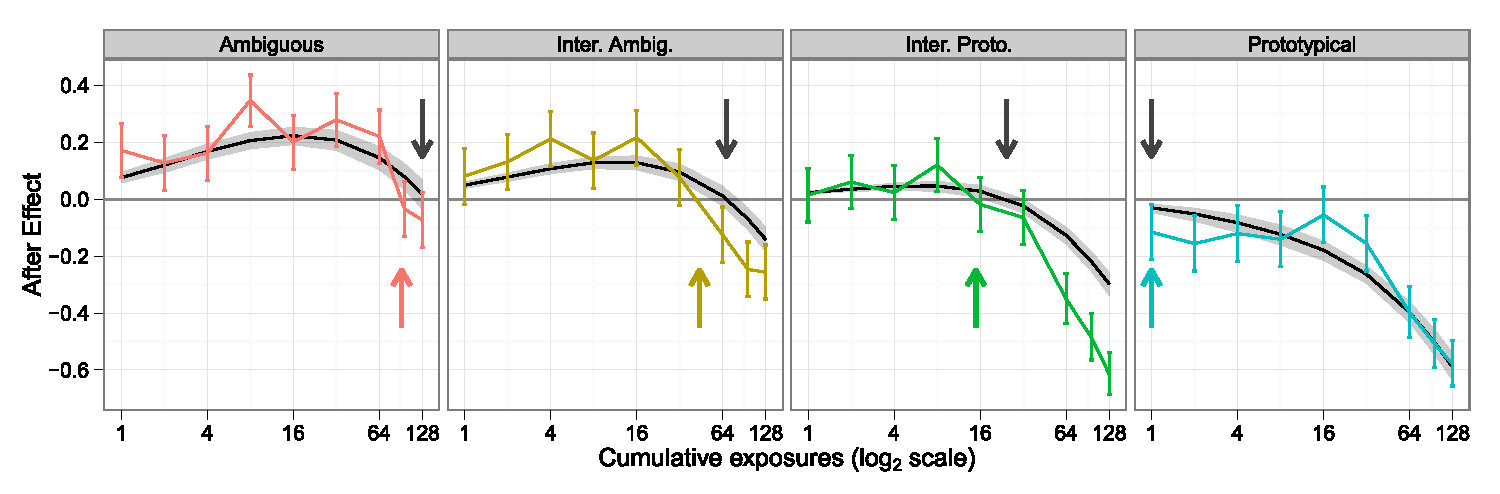
\includegraphics[width=\textwidth]{intr-model-ae-firstblock-xover-arrows.pdf}
  \caption{Results from all four conditions in the first exposure block: ambiguous, intermediate-ambiguous, intermediate-prototypical, and prototypical (colored lines with error bars showing 95\% confidence intervals). Model fits (black lines with 95\% confidence interval ribbons) are generated based \emph{only} on the ambiguous and prototypical conditions ($r^2=0.91$); for the two intermediate conditions the model makes the predictions shown ($r^2=0.96$).  Colored arrows show the amount of exposure required for behavior to switch from recalibration-like (positive after-effect) to selective adaptation-like (negative after-effect), which decreases as the adaptor stimulus goes from ambiguous to prototypical, as predicted by the model (black arrows; see Figure~\ref{fig:cross-over-scatterplot}).}
  \label{fig:intr-results-fits}
\end{figure}

Here we focus on the evaluation of the incremental belief updating model developed in the previous sections. Additional data analyses confirmed that our web-based design replicates the results of \citeA{Vroomen2007} and further supports our interpretation of the data. These analyses can be found in the Supplementary Material to this article.\footnote{The Supplementary Material are available from \url{http://www.bcs.rochester.edu/people/dkleinschmidt/pubs/KleinschmidtJaeger-SupplementaryMaterial.pdf}}
Figure~\ref{fig:intr-results-fits} shows the results from the four conditions, along with the predictions from the model fit to the ambiguous and prototypical conditions.  First, our results replicate those of \citeA{Vroomen2007}.  Exposure to the prototypical adaptor leads to negative aftereffects which build up gradually and become stronger throughout exposure, while the exposure to the ambiguous adaptor leads to positive aftereffects which peak and eventually fade, becoming negative after 128 exposures (see Supplementary Material).
In fact, the recalibration decline that we find is even stronger than that found by \citeA{Vroomen2007}, with 128 exposures being enough to almost completely erase any positive aftereffect.  \citeA{Vroomen2007} observed such a reversal after 256 exposures in their full data set, but only a slight dip in the strength of the recalibration effect by the end of the first block of exposure (Figure~\ref{fig:vroomen-results-256}).
Our belief updating model fits the data from the ambiguous and prototypical conditions quite well \autocite[$r^2=0.91$ overall, vs. $r^2=0.93$ when fit to][]{Vroomen2007}.

Second, these results validate the predictions of the belief updating model for intermediate conditions, both qualitatively and quantitatively.  Qualitatively, as predicted, the two intermediate conditions reveal that the ambiguous and prototypical conditions are endpoints of a continuum of adaptation effects.  This is visually clear from Figure~\ref{fig:intr-results-fits} and also borne out by statistical analysis (see Supplementary Material). %(Appendix~\ref{sec:interm-cond}).
Quantitatively, the belief updating model hyperparameters that were fit \emph{only} to the ambiguous and prototypical conditions accurately predict the adaptation build-up in the two intermediate conditions.  In fact, the fit to the intermediate conditions is as good as the fit to the conditions the model was trained on ($r^2=0.96$ for the two intermediate conditions vs. $r^2=0.91$ for the ambiguous and prototypical).  This is encouraging given that individual participants show substantial variability in their adaptation behavior and each condition consisted of an entirely different group of participants.

\begin{figure}[htb]
  \centering
  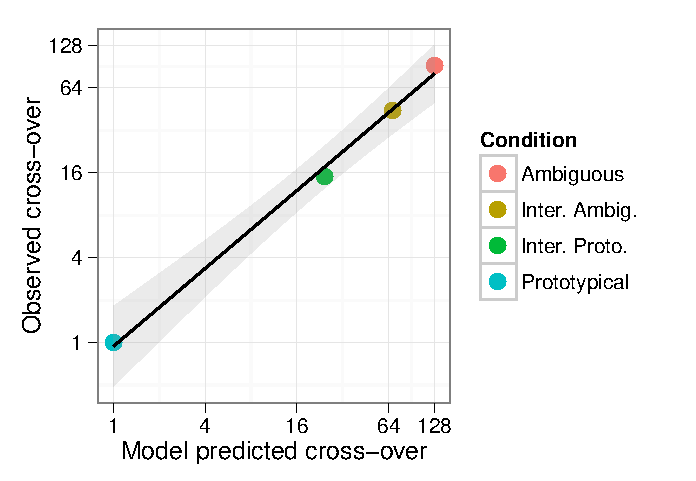
\includegraphics[width=0.75\textwidth]{intr-ae-firstblock-xover-scatter-logscale.pdf}
  \caption{The belief-updating model predicts when behavior should switch from recalibration-like to selective adaptation-like (see Figure~\ref{fig:intr-results-fits}).  Each dot shows the model predicted cross-over point ($x$-axis) versus the actual observed cross-over point ($y$-axis), with a linear regression fit to these four points showing close agreement.}
\label{fig:cross-over-scatterplot}
\end{figure}

We can further compare the model predictions and the data by looking at the point at which the aftereffect crosses over from being positive (recalibration-like) to negative (selective-adaptation-like).  In Figure~\ref{fig:intr-results-fits}, these cross-over points are indicated by arrows---black for the model predictions and colored for the data---and Figure~\ref{fig:cross-over-scatterplot} shows that the observed and model-predicted cross-over points are strongly correlated, even though the cross-over point itself was not explicitly fit to the data.  Thus, the belief updating model very effectively predicts the point at which behavior switches from recalibration-like to selective-adaptation-like for intermediate adaptors of varying ambiguity, based solely on the fit to ambiguous and prototypical adaptor data.

The best-fitting (MAP estimate) effective prior sample sizes for the category variances and means were small: $\nu_0 = 88$ and $\kappa_0=2.9$, respectively.  This again closely resembles what we found for the \citeA{Vroomen2007} data.  It also corroborates the conclusion that participants in these studies consider their previous experiences with \ph b and \ph d to be not particularly relevant in these situations, 
and moreover replicates the finding that, for these stimuli and this experimental paradigm, listeners seem to place more confidence in their prior beliefs about the category variances than the means ($\nu_0 > \kappa_0$ both here and in all previous model fits).  Finally, as with the data from \citeA{Vroomen2007}, the best-fitting cue combination weight had audio and visual cues weighted roughly equally, placing in this case slightly more weight on the visual component ($w=0.63$).\footnote{The slightly higher weight for visual cues in our data might be a consequence of using stimuli derived from a Dutch /b/-/d/ continuum, which are similar but presumably not identical to those typically experienced in American English.}

\subsection{Discussion}
\label{sec:discussion-3}

These results demonstrate two points.  First, by replicating the results of \citeA{Vroomen2007}, they show that web-based platforms are a viable way to investigate phonetic effects such as recalibration and selective adaptation which depend on the particular acoustic parameters of the stimuli.  Most participants were enthusiastic and engaged in the study, and using sensible exclusion (based on pre-test performance or catch trials during exposure) those who are not fully attentive or who cannot hear the stimuli properly can be excluded.

Second, the ideal adapter framework for understanding phonetic adaptation presented above can explain both the phonetic recalibration \emph{and} selective adaptation data from \citeA{Vroomen2007} based on the mean (ambiguous vs. prototypical) and variance (none) of the adaptor distributions.  This framework predicts that intermediate adaptors should produce intermediate adaptation effects, and moreover, the formal, quantitative model based on these principles makes specific, quantitative predictions about the effect of cumulative exposure to these intermediate adaptors.  Both these qualitative and quantitative predictions were borne out in the data presented here.

\section{Concluding Part I: Adaptation as inference under uncertainty about the statistics of the generative model} 
\label{sec:conclusion-part1}

In this first part of this article, we have formulated the ideal adaptor framework, building on previous work on speech perception within the ideal listener framework \cite{Clayards2008,Feldman2009a,Norris2008,Sonderegger2010}. We have applied the ideal adaptor framework to two phonetic adaptation phenomena commonly considered to be due to distinct mechanisms, perceptual recalibration and selective adaptation. To do so, we derived a Bayesian belief updating model from the ideal adaptor. This framework allowed us to formalize the intuition that perceptual recalibration is a form of distributional (statistical) learning that changes the underlying representations of phonetic categories \cite<e.g.,>{Norris2003,Kraljic2005,Maye2008a,Bertelson2003}. The Bayesian belief updating model provides a good quantitative fit to perceptual recalibration data ($r^2\mathrm{s}> .8$). The model also qualitatively captures the cumulative effect of exposure in perceptual recalibration experiments, including the previously observed reversal of initial effects after prolonged exposure to the same stimulus \cite{Vroomen2007}.

Going beyond perceptual recalibration, the model suggests selective adaptation, too, is at least in part due to distributional learning similar or identical to that observed during perceptual recalibration. In addition to good quantitative and qualitative fits to selective adaptation data, our Bayesian belief updating model predicted a continuum from selective adaptation to perceptual recalibration, which was indeed observed. This serves as a demonstration of the ability of the ideal adapter framework to make quantitative predictions that go beyond existing data.

It is worth mentioning that the \emph{model} which is used to generate those predictions in this case makes many assumptions that are not intrinsic to the framework but rather are made for convenience, tractability, or to better illustrate the basic mechanics of belief updating (for discussion, see the Appendix). These assumptions are largely justified for this particular experimental paradigm (see Table~\ref{tab:model-assumptions} in the appendix). They must, however, be considered carefully when thinking about how this particular \emph{model} might generalize to other paradigms. Support for the ideal adaptor framework as a general framework of adaptation beyond the type of experimental paradigms considered here comes from research finding qualitatively similar patterns of speech adaptation in situations that more closely resemble the complexity of every day speech perception \cite{Eisner2006,Reinisch2014}.

\subsection{Novelty of the ideal adapter: Putting learning front and center}
\label{sec:novelty-ideal-adapt}
\label{r2-part1-novelty}

Many of the ideas we have discussed so far are anticipated in more or less explicit form in previous work on speech perception.  Our approach to speech perception is novel in two ways.  First, the ideal adapter puts learning front and center in speech perception, as an unavoidable consequence of the combination of the task of the speech perception system---mapping cues to categories---and the world where that task is carried out---where the cue-category mapping varies from one situation to the next.  In this way of looking at the speech perception system, learning or adaptation is a necessary part of normal speech perception.  Existing models of speech perception---Bayesian and otherwise---for the most part do not learn or adapt \cite{Clayards2008,Feldman2009a,McClelland1986,Norris1994,Norris2000}.  This is, in general, not an in-principle limitation of these modeling frameworks, but rather reflects simplifying assumptions made for the sake of tractability in previous work.  

There are only a few models of speech perception that learn,\footnote{Leaving aside for the moment models of \emph{acquisition}, which we will discuss below.} all of which have been proposed in recent years based on findings that speech perception is highly flexible \cite{Lancia2013,Mirman2006}.  These models are connectionist models that adjust feedforward weights from acoustic cues to phonetic categories using Hebbian mechanisms.  
We postpone further discussion of these models until Part III below, except to say that they have only been applied qualitatively to the asymptotic effects of phonetic recalibration (if they have been directly applied to phonetic recalibration at all).  As such, it is not clear whether they can, like the belief updating model we present here, simultaneously account for selective adaptation as well, or the detailed effects of cumulative exposure on the size and direction of phonetic adaptation.  Another class of models that are broadly compatible with the ideal adapter is episodic or exemplar models \cite<e.g.,>{Johnson1997a,Goldinger1998,Pierrehumbert2003}, which learn the distribution of sounds corresponding to linguistic units implicitly by storing raw acoustic traces.  However, as we will discuss at length in Part II, despite similar motivations, the ideal adapter framework differs in an important way, because it abstracts away from individual episodes, both at the level of phonetic categories (or some other sublexical level of representation) and at the level of individual talkers and groups of talkers.

A deeper problem with existing models---even those that learn---is that they don't address how listeners manage to balance stability and plasticity in speech perception.  Rather, learning rate is treated as a free parameter which is tuned such that the model behaves in a reasonable way.  A model of the speech perception system ultimately has to address how stability and plasticity are balanced, because there is a wealth of evidence that people manage to do this very well.  While the belief updating \emph{model} we have presented above has free parameters that control the learning rate (the prior confidence parameters) and which were fit to the data, the ideal adapter \emph{framework} provides a more principled way to approach the stability-plasticity trade-off, which we turn to in the second, more speculative and forward-looking part of this paper.  





\section*{Part II}
\label{sec:part-ii}

Human speech perception is characterized by both extreme flexibility and stability.  Listeners can rapidly adapt to a novel pronunciation while not losing the ability to efficiently comprehend standard pronunciations.  Part II of this paper focuses on the balance between stability and flexibility, and in particular how---in the ideal adapter framework---it is related to the structure of the world that the speech perception system has to operate in.  There are two main aspects to this structure.  

First, the generative model---the statistical properties of speech sounds for each phonetic category---can be \emph{different} from one situation to the next.  If the listener's beliefs about these statistics are substantially different from the current situation's actual generative model, then comprehension can be slowed or even incorrect.  Situation-by-situation differences in the generative model require that listeners continuously infer the appropriate generative model, combining their prior expectations with current observations. 
In Part I we illustrated how phonetic adaptation can be understood as incremental belief updating, focusing intentionally on novel situations where listeners' prior experience was not likely to be very informative, allowing the influence of each additional observation to be seen more clearly. 

However, there is a second relevant aspect to the speech perception system: generative models do not vary \emph{arbitrarily} across situations, but are rather tied to, for example, \emph{who} is talking.  This means that listeners can expect to encounter the same---or similar---generative models again and again (and some more than others).  In Part II of this paper, we focus on these \emph{similarities} across situations that a listener encounters in the world, and discuss how the ideal adapter framework links this structure---with both predictable and unpredictable variation in generative models---with the stability and flexibility of the speech perception system.  While a lot of future work is required to flesh out a computational cognitive model, we will present a tentative outline of how the ideal adapter framework formalizes the link between the distribution of generative models in the world, listeners' prior expectations, and their behavior.  The ideal adapter framework's basic predictions are qualitatively supported by the available behavioral evidence.  At the same time, the ideal adapter framework identifies a number of questions that we consider particularly critical for future research.

\subsection{Recognize the familiar}
\label{sec:recognize-familiar}

While we have assumed that adaptation to a novel talker does not start from scratch, but rather from some form of prior beliefs about phonetic distributions (literally, the prior in the Bayesian belief-updating model introduced in Part I), we have so far paid little attention to the properties of this prior knowledge.  For the examples entertained in Part I, such as the speech a listener is exposed to in a perceptual learning experiment, the specific prior beliefs that the listener brings to the situation are of little consequence because they will quickly be overwhelmed by the input listeners receive from the novel talker. In everyday life, however, listeners will not only encounter talkers that differ starkly from previously experienced talkers. Instead, some talkers will have been encountered before and others will resemble previously experienced talkers to varying degrees. This means that {\em different aspects} of previous experience bear more or less strongly on the current situation. How listeners determine which previous experiences are the most relevant in a given situation is one of the goals of the second part of this article. 

Consider, for example, what happens when you walk into a room where your best friend is talking.  You can recognize them based on a variety of things, perhaps including their face, distinctive clothes they happen to be wearing, the fact that they are standing in a room in their own house, or the timbre of their voice.  Because every individual speaks slightly differently, your best friend sounds different from other talkers, and it would be beneficial to be able to just ``swap in'' their particular cue statistics based on your vast experience with their speech in the past.  Anecdotally, this is what happens when we encounter a highly familiar talker, and indeed it is broadly accepted and empirically supported that we have such talker-specific representations, and use them online in speech perception \cite{Creel2008,Creel2011,Goldinger1996,Nygaard1998,Palmeri1993,Remez1997}, although questions remain about the limits of this ability \cite{Magnuson2007a,Pardo2006}.

Talker-specificity in speech perception reveals an important insight: knowledge about the statistics of speech cues needs to be \emph{structured} to provide the full benefit to the listener.  This has long been recognized by, for example, exemplar-based theories of speech perception, where storage of rich acoustic details of each episode leads naturally to persistent, talker-specific representations of the variability of speech sounds, either implicitly or explicitly \cite{Goldinger1996,Goldinger1998,Johnson1997,Johnson2006,Pierrehumbert2003}.  In the language of the ideal adapter framework, the presence of talker-specificity means that, far from simply being engaged in continuous statistical learning, listeners are in fact using their previous experience to at the very least determine where to \emph{start} such statistical learning in each situation. It is this second type of inference---inferences about what aspect of previous experience are most relevant to the current situation---that prevents listeners from having to re-adapt from scratch every time they encounter a talker (whether it is a novel talker or a previously encountered one). Although the existence of talker-specific knowledge is now broadly accepted, the consequences that the existence of such knowledge has for understanding speech perception is perhaps still under-appreciated. Specifically, most previously proposed models of speech perception, with the exception of certain exemplar-based approaches \cite{Goldinger1998,Johnson1997,Pierrehumbert2003}, either do not learn \cite{Clayards2008,Feldman2009a,Norris2008} or are what we will call `flat' learners, without the ability to induce structure over talkers \cite{Feldman2013a,Lancia2013,McMurray2009,Mirman2006,Vallabha2007}. These models are insufficient to account for talker-specificity and related phenomena discussed below.  Even looking beyond speech perception into the burgeoning literature on learning in the face of (latently) non-stationary statistics \cite<e.g.,>{Cho2002,Gallistel2001}, most existing models cannot account for some of the basic properties of speech perception discussed here.\footnote{This also makes speech perception a potentially productive test domain for further development of general models of learning in a non-stationary world.} We return to this point below, as it motivates the proposal we lay out in this second part of the article.

\subsection{Generalize to the similar}
\label{sec:generalize-similar}

There is also evidence that the structure of listeners' previous knowledge extends beyond the level of particular individual talkers.  To take a somewhat extreme example, one of our colleagues moved from New York to Northern England, where a very different dialect of English is spoken.  Initially, he had a great deal of difficulty understanding what anyone was saying, but after some number of months he found that it became easier to comprehend this accented speech, even when it was spoken by particular individuals he had never met before (Farmer, \emph{personal communication}).  In the language of the ideal adapter, we might say that our colleague learned something about how the cue statistics---or generative models---vary across individual talkers who share this accent, and that this gave him a head start in adapting to a new, but similarly-accented talker.  Although somewhat less well-studied than talker-specificity, there is some evidence that people are broadly capable of such generalization, using their experience with groups of talkers to guide speech perception \cite{Bradlow2008,Baese-berk2013,Creel2011,Johnson1999,Johnson2006,Niedzielski1999,Sidaras2009}.  There are, in the world, a range of structures that group talkers, from common language community (leading to dialect and accent groups) to factors like gender or sexual orientation \cite{Munson2007}.
The ideal adapter predicts that listeners should pick up on, and take advantage of, these groupings, to the extent that they are informative about the generative models of the corresponding talkers.

In order to take advantage of the structure of how generative models vary in the world, listeners need to \emph{learn} this structure through experience.  Listeners do not directly know how generative models are distributed in the world, just like they do not have direct access to the generative model behind each utterance they observe.  This makes the problem of how to take advantage of any structure that might be there in the world another problem of inference under uncertainty.   It is clear that listeners need to learn in order to group talkers together, since meeting two talkers with similar generative models could just be a coincidence, but meeting twenty such talkers likely indicates some underlying dialect group.  However, this kind of higher-level learning is also required for talker-specificity.  That is, in order to benefit from experience with a new talker in future occasions, listeners cannot just adapt to that talker's generative model for the current situation, but rather must, after sufficient exposure, remember what they have inferred about that particular talker's speech statistics so that they can deploy that knowledge on future encounters.  The need for listeners to induce structure over their previous experiences with different generative models suggests that despite being rapid, adaptation---like that discussed in Part I---should persist because it reflects the listener's attempt to build a model of the current situation which can be useful in the future.  This is another way of saying that phonetic adaptation is not just priming but a form of learning about the situation and/or talker \cite[among others]{Eisner2006,Kraljic2005,Kraljic2008a}.

\subsection{Outline for Part II}
\label{sec:outline-part-ii}

\label{r-formalization-benefits}
We will expand on these intuitions about how listeners can benefit from picking up on the structure of their experience with different cue statistics, and review the relevant literature.  Our first goal is to argue that the ideal adapter framework provides a unifying view that ties together a range of previously stated intuitions and proposals about talker-specificity, generalization, and adaptation in speech perception.  Our second goal is to lay out a preliminary formalization of the ideal adapter framework as it relates to how a listener could take advantage of structure in their prior experience.  While we will not present any implemented, quantitative model simulations like in Part I, we believe that formalizing the framework has a number of advantages.  First, it will highlight the computational parallelism between recognizing familiar talkers, generalizing to similar talkers, and what we've called adaptation to novel talkers in Part I, all of which reflect listeners' attempts to infer the appropriate generative model for the current situation.  Second, having a formalization of a theory can sometimes help when our theoretical intuitions break down, such as when, for instance, speech perception is \emph{not} talker-specific \autocite[e.g.][]{Kraljic2007}.  Third, formalizing can help guide future research.  As will become clear below, the ideal adapter framework puts a major emphasis on statistics of the speech signal, and how those statistics differ across talkers and groups of talkers \emph{in the world}.  Relatively little research has looked at this, and the ideal adapter framework provides a potentially productive link between this kind of data and human behavior.

Part II is organized into four main sections, each of which addresses a different aspect of how the listener's need to infer the appropriate generative model in each situation results in different strategies based on the information available to them from structure in the world (via prior experience) and the speech they observe in that situation.  First, we focus on how listeners can benefit from familiarity with a particular talker.  Maintaining and using talker-specific beliefs about generative models allows listeners to forgo adaptation altogether when they encounter a familiar talker again.  Second, we ask how listeners get to the point of having such talker-specific beliefs.  Every familiar talker was once novel, and became familiar through experience.  Combining the belief-updating logic that was the focus of Part I with talker-specific beliefs leads to the ideal adapter's prediction of talker-specific adaptation.  Third, we turn to the question of where a listener \emph{starts} when adapting to an unfamiliar talker.  Even if a particular individual is unfamiliar, the listener often has experience with other similar talkers that can be informative.  We will discuss evidence that listeners are indeed sensitive to this information, and how it can be formalized in the ideal adapter framework.  Fourth, and finally, we tie all three strategies together, and discuss how connections between adaptation, recognition, and generalization are demonstrated by how listeners behave when they are not entirely sure what prior experience is more relevant.  


\section{Recognizing the familiar: Talker-specificity}
\label{sec:recogn-famil-talk}


We begin with situations in which stable beliefs about the generative model are maximally beneficial: particular familiar talkers.  Listeners can benefit from experience with a familiar talker to the extent that they consistently use a particular generative model---producing certain cue distributions---that is different from other talkers.  By maintaining stable representations of that talker's particular generative model, the listener would be able to deploy those representations when the talker is encountered again in the future, removing the need to adapt to them again.  If, as the ideal adapter predicts, listeners are taking advantage of this structure---that talkers tend to use the same generative model consistently---then listeners should generally process speech in a talker-specific way, and specifically should process speech from familiar talkers faster, more accurately, and more robustly.

\subsection{What do we know about talker-specificity?}
\label{sec:what-do-we-know-talker-spec}

Talker-specificity is one of the best-studied and uncontroversial features of human speech perception.  Talker-specificity is observed both in the form of the ability of listeners to explicitly identify particular individual talkers based on their speech, even when it is highly degraded \cite{Bricker1966,Palmeri1993,Remez1997,Sheffert2002}.  Offline measures of speech processing also show talker-specificity.  For instance, words are better remembered when they're spoken by the same talker at study and test \cite{Goldinger1996,Palmeri1993}.  However listeners also use talker-specific information to benefit processing.  Listeners are faster and more accurate at comprehending speech in noise when it was produced by familiar talkers, both for unaccented \cite{Nygaard1998} and accented \cite{Clarke2004} talkers.  These effects seem to operate at a low level in speech perception, with online measures like eye-tracking suggesting that listeners use experience with talker-specific productions as early as it is possible to detect \cite{Creel2008,Mitterer2013}.

\begin{figure}[htb]
  \centering
  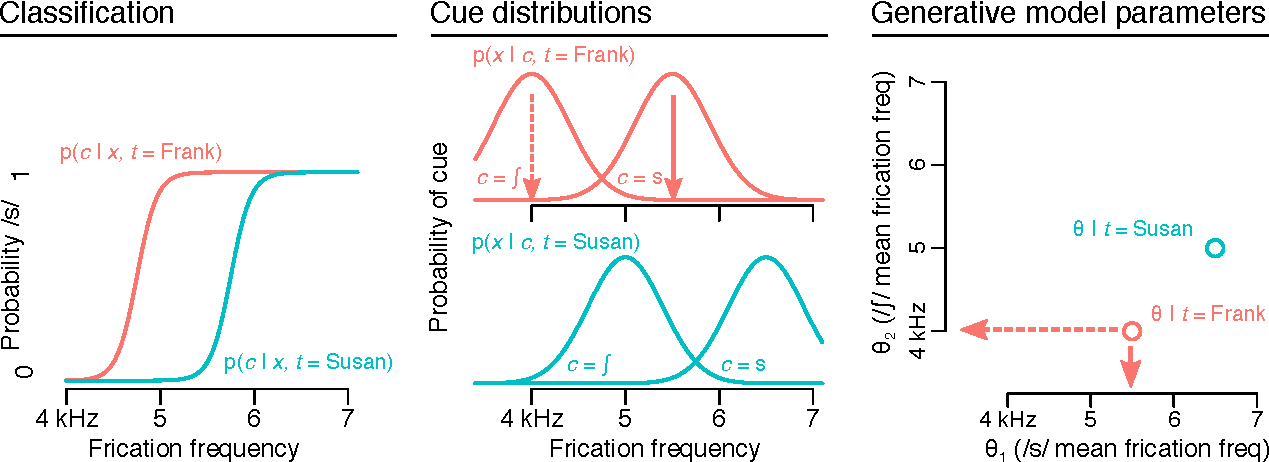
\includegraphics[width=\textwidth]{part2-schematics/part2-fig1-assembled.pdf}
  \caption{Talker-specific speech perception can be formalized as inference under uncertainty conditional on talker identity.  The probability that a particular cue value $x$ (here, frication frequency) was intended to be category $c$ (\ph s or \ph S) depends on the talker $t$ that produced it, written $p(c \given x, t)$ (left).  This probability is related via Bayes Rule to the talker-specific likelihood, the distribution of cues produced by talker $t$ for each category, $p(x \given c, t)$ (middle).  These distributions can be described by the \emph{parameters} of the generative model, $\theta$, such as the talker's mean frication frequency for \ph s and \ph S as plotted (right).  Although we only plot two parameters, many more are required to even approximate the full generative model.  Each talker can be thought of as a point in this (very high dimensional) parameter space.}
  \label{fig:gen-model-points}
\end{figure}

\subsection{How does the ideal adapter formalize talker-specificity?}
\label{sec:how-does-ideal-adapter-talker-spec}

We can formalize the intuition that listeners use talker-specific information to guide speech perception within a Bayesian inference framework in the following way (visualized in Figure~\ref{fig:gen-model-points}).  Speech perception is treated as an inference process, where the listener is trying to infer the talker's intended category $c$ (or message, more generally), given some acoustic observation $x$.  As discussed in Part I, this relationship is probabilistic, due to unavoidable variability in production and sensory uncertainty, and we can express the cue-to-category inference using Bayes' rule, as in Equation~\eqref{eq:1}, as a combination of how likely a category is \emph{a priori} (the prior), and how well it predicts the observation (the likelihood).  Talker-specific information can come into play in both the prior and the likelihood.  If a talker is more likely to produce \ph s (overall or because of lexical preferences), this should be taken into account in the prior probability assigned to \ph s.  More importantly, given that each talker might produce a different distribution of cues for \ph s, the \emph{likelihood} of any given observation also depends on the talker.\footnote{The belief-updating model implemented in Part I only models changes in the likelihood.} Treating both the likelihood and prior as conditional on the talker (denoted $t$) results, after applying Bayes rule, in a talker-specific posterior over possible intended categories: 
\begin{equation}
  \label{eq:23}
  p(c \given x, t) \propto p(x \given c, t) p(c \given t)
\end{equation}
This is shown schematically for classifying a VOT value as \ph s or \ph S in Figure~\ref{fig:gen-model-points}: different talker-specific cue distributions (middle) result in different category boundaries (left).

However, this way of formalizing talker-specificity doesn't exactly capture the fact that the likelihood $p(x \given c, t)$---the distribution of cues for each category---depends on the talker's \emph{generative model}, rather than the talker's \emph{identity} per se.  We can represent a particular generative model with a vector of its parameters---things like the mean VOT for \ph b, the variance of the frication frequency for \ph s, etc.---jointly denoted as $\theta$.\footnote{\label{note:gen-mod-params}We represent the generative model via a list of its parameters as a notational convenience, and not to make any claims about whether or not the listener's actual generative model is a \emph{parametric} model, where each category is, for instance, a normal distribution over its cues.  Formally, we simply mean the parameters $\theta$ to be a description of the generative model, which might be as compressed as a vector listing the mean and variance of each category on each cue dimension, or as fine-grained as an infinitely long vector which just lists the actual likelihood assigned by each category to each possible sound.}  If the listener knew, exactly, the talker's actual generative model, then we could write the talker-conditional likelihood as directly conditional on that actual generative model: 
\begin{equation}
  \label{eq:26}
  p(x \given c, t) = p(x \given c, \theta=\theta_t)
\end{equation}
Of course, we have argued above that listeners in general do \emph{not} have direct access to the exact generative model, but rather some uncertain beliefs about it.  That is, the listener's knowledge about the talker $t$'s generative model is better described as a probability distribution, $p(\theta \given t)$, rather than a single value, $\theta_t$ (Figure~\ref{fig:gen-model-points}, right).  One consequence of this is that the talker-specific likelihood should, ideally, take into account this uncertainty by averaging the likelihood assigned by each possible generative model $p(x \given c, \theta)$, weighted by how likely the listener thinks that particular generative model is for talker $t$, $p(\theta \given t)$:\footnote{This further assumes that the listener recognizes talker $t$ with complete certainty.  In many cases, this is a reasonable simplifying assumption, but in many others it is not, and we will address the consequences of this in a later section.} 
\begin{equation}
  \label{eq:27}
  p(x \given c, t) = \int p(x \given c, \theta) p(\theta \given t) \ud \theta
\end{equation}

\label{r2-talker-spec-novelty}
Making beliefs about the generative model parameters explicitly conditioned on talker identity introduces another level of structure above and beyond the belief-updating model in Part I.  That model simply sought to infer the appropriate generative model parameters based on some, overall beliefs about what parameters were likely overall---the prior $p(\theta)$---and how well the current speech was explained by each possible generative model---the likelihood $p(x \given \theta)$.  The belief-updating model from Part I (implicitly) thus assumes that the same prior beliefs would be relevant, no matter the situation, and \emph{all} that it can do to adapt to the current situation is to update its beliefs through distributional learning.  This makes the incremental belief updating model and other flat learning models---such as simple recurrent networks, \cite{Chang2006,Elman1990}, other connectionist models without further assumptions, \cite{Mirman2006,Lancia2013}, non-hierarchical reinforcement learning, \cite{Gallistel2001}, etc.---insufficient to account for some of the most basic properties of speech perception.

However, if listeners have prior beliefs that are specific to---conditioned on---a particular familiar talker, then they do not need to bring exactly the same beliefs to every situation.  Rather, by \emph{recognizing} a familiar talker they can deploy the corresponding talker-specific prior beliefs to ``adapt'' to the current situation without needing to actually go through the process of distributional learning.  In the next section, we will explore the question of how listeners get to the point of having beliefs about a particular talker's generative model, but first we discuss what we see as some of the most pressing issues for future work that this raises.

\subsection{Open questions: talker-specificity}
\label{sec:open-quest-talk}

One of the consequences of thinking about talker-specific beliefs as distributions over generative models is that the inevitable uncertainty of these beliefs might lead to further uncertainty in how speech is classified, above and beyond the inherent uncertainty from the probabilistic nature of speech perception itself.  As a result of having only uncertain beliefs about a talker's generative model, a truly ideal adapter would have more uncertainty about how to categorize a particular cue value when they are less certain about the talker's generative model.  This could result in, for instance, shallower category boundaries than predicted by a true ideal listener with perfect knowledge of the generative model.  We should stress here that maintaining uncertainty is not per se a bad thing.  To the contrary, properly accounting for uncertainty about the talker's intended message is a strength of this approach, and it would be far worse to be overly-confident about a classification that turns out to be wrong.  Under this view, because listeners should have less uncertainty about highly familiar talkers, classification behavior should be closer to what is predicted by the actual cue distributions.  Alternatively, listeners might not take into account their full uncertainty in the generative model, and go with their best guess rather than averaging over the full distribution.  Other intermediate approximations are possible, with the listener considering only a finite number of different possibilities.  
While processing of familiar talkers is overall faster and more accurate, we do not know how this is reflected in the detailed patterns of categorization behavior, which is required to effectively evaluate how much uncertainty listeners are maintaining about the current generative model.
Working out the implications of these various ways of dealing with uncertainty is thus in our view a pressing topic for future work, both computational and behavioral.  

\label{r4-context-specific-adaptation}
Another question is whether talker-specific beliefs about the generative model are something that is unique to speech perception, or instead reflects more general perceptual strategies.  That is, here we have focused on \emph{talker}-specificity. However, the ideal adapter framework in principle predicts that listeners might form beliefs about any type of re-encountered situation/context, if these context/situations are reliably associated with systematically different speech statistics (generative models) and encountered sufficiently frequently. This could include beliefs about being in certain types of spaces (an echoey cathedral, a wide open field, a room with a light that buzzes at particular frequency, etc.).  Of course, many of these properties are relevant to many other sorts of auditory processing, like sound source localization, and the use and deployment of context-specific beliefs about cue statistics might not be something that is unique to speech processing.  Rather, they may reflect a general property of both higher- and lower-level sensory processing, so that the relevant inference might occur below the levels we have so far considered.  


\section{Learning talker-specificity through adaptation}
\label{sec:learn-talk-spec}

So far, we've discussed the benefits of talker-specific knowledge (and how it can be formalized in the ideal adapter framework) assuming that the listener \emph{is} familiar with some talkers and their particular cue statistics (generative models).  But of course listeners start off knowing very little about a particular talker's generative model, and so in order to be able to make use of talker-specific cue statistics, listeners need to learn about those statistics from experience.  In Part I, we discussed evidence that listeners rapidly adapt to cue statistics in a novel situation, as predicted by the ideal adapter faced with the lack of invariance.  However, if a listener \emph{only} adapted, then they would never be able to develop the sort of talker-specific representations that are now generally accepted to be a basic feature of the speech perception system.  The ideal adapter framework thus also predicts that, when faced with the need to learn such talker-specific representations, listeners do not \emph{just} adapt in the short term, but hold onto their updated beliefs about the generative model for whatever talker (or kind of situation, more generally) that they have adapted to.  

\subsection{What do we know about talker-specific adaptation?}
\label{sec:what-do-we-know-talker-adapt}

Despite being very rapid, phonetic adaptation has been found to lead to stable, persistent representations.  This suggests that rapid phonetic adaptation is, in many cases, better thought of as the result of listeners learning something about the talker they encounter in the experiment.  A prime piece of evidence for this is that the effects of phonetic adaptation can remain strong even after intervening exposure to speech from another talker \cite{Kraljic2005,Kraljic2007}, even after leaving the laboratory and returning 12 hours later \cite{Eisner2006}.\footnote{While there are some situations in which intervening speech from another talker \emph{does} disrupt adaptation \cite<e.g. the \ph d-\ph t condition in>{Kraljic2007}, this is broadly consistent with the more general prediction of the ideal adapter that listeners are tracking the overall distribution of generative models across situations, which we discuss below.}  Moreover, there's also some evidence that listeners can learn separate generative models for two different talkers in the same situation, even when utterances from the two talkers are mixed together \cite{Munson2011}.  This would not be possible if listeners were simply tracking the short-run statistics of particular acoustic cues like VOT.

\subsection{How does the ideal adapter formalize talker-specific adaptation?}
\label{sec:how-does-ideal-form-talker-adapt}

In the ideal adapter framework, this sort of talker-specific adaptation follows naturally from the idea, introduced in the last section, that listeners are using talker-specific beliefs about the generative model.  Talker-specific beliefs about the generative model are updated in a similar way as in the ``flat'' belief-updating model introduced in Part I: by bringing the cue statistics predicted by the generative model into better alignment with the observed cue statistics.  The only difference is that instead of considering the statistics of \emph{all} observations (as the belief-updating model of Part I implicitly does), the listener should consider only the statistics of observations produced by a particular talker in updating their beliefs about that talker's generative model.

\begin{figure}[!htb]
  \centering
  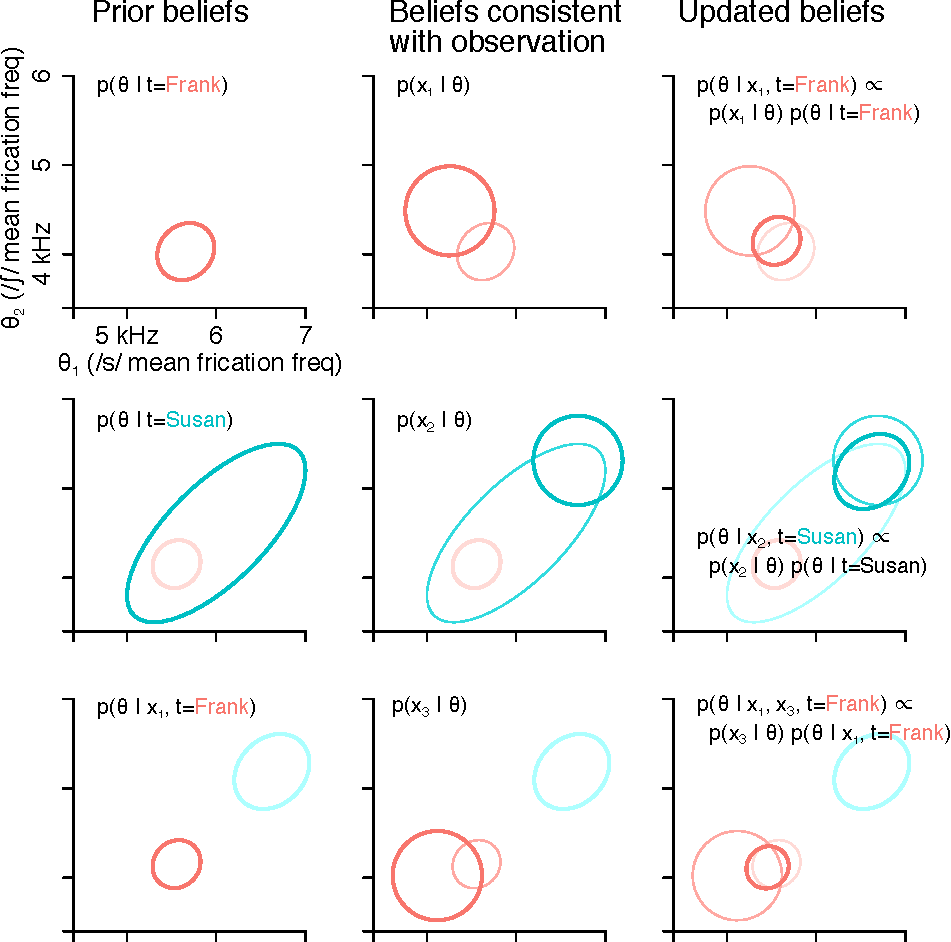
\includegraphics[width=0.75\textwidth]{part2-schematics/talker-specific-belief-updating-annotated.pdf}
  \caption{Adapting to multiple talkers: Updating of talker-specific beliefs allows listeners to continue to learn about individual talkers' generative models by accumulating evidence over multiple encounters.  These plots visualize beliefs about generative models as distributions in generative model parameter space (here, showing only mean frication frequencies for \ph s and \ph S).  Each panel plots equiprobability contours of a distribution (that outline the highest probability region of generative model parameter space), based on prior experience (left column), a single observation (middle), and their combination after belief updating (top).  Top row: updating beliefs about a familiar talker (``Frank''), starting from relatively specific beliefs (left).  A single observation $x_1$ is compatible with a wide range of generative models (middle), but when combined with prior beliefs leads to more specific updated beliefs.  Middle row: updating beliefs about a new talker (``Susan''), encountered next, based on very vague prior beliefs and the next observed speech $x_2$.  Bottom row: continuing to update beliefs about Frank---which are not affected by the intervening speech from Susan---after observing another cue value $x_3$.}
  \label{fig:talker-specific-belief-updating}
\end{figure}

Such talker-specific belief-updating is formalized in generally the same way as it was in the belief-updating model in Part I.  For each observation $x$ from talker $t$, the listener updates their uncertain beliefs about talker $t$'s generative model, $p(\theta \given t)$, by combining them with information about which generative models are more or less compatible with the observation $x$:\footnote{Really, the listener's inference about the intended category depends on their inference about the generative model parameters, and vice versa; see Equation \eqref{eq:12}.  Here we average over (marginalize out) possible category interpretations of $x$ for simplicity's sake, as in Equation \eqref{eq:18}.}
\begin{equation}
  \label{eq:28}
  p(\theta \given t, x) \propto p(x \given \theta) p(\theta \given t)
\end{equation}
Note that, as in Equation~\eqref{eq:27}, the dependence on the talker is entirely driven by the talker-specific beliefs about the generative model; given a particular value of the generative model parameters, the talker's identity doesn't change the likelihood of an observation $x$.
These updated beliefs can then be further updated with other observations, with the updated beliefs after the first observation $x_1$ from talker $t$ serving as the starting point for updating beliefs after hearing another observation from talker $t$, $x_2$: 
\begin{equation}
  \label{eq:29}
  p(\theta \given t, x_1, x_2) \propto p(x_2 \given \theta) p(\theta \given t, x_1)
\end{equation}
In this way, the ideal adapter can combine information from multiple encounters with talker $t$, even if they are separated by intervening speech from other talkers (Figure~\ref{fig:talker-specific-belief-updating}).  Combining information from different encounters with a single talker is important for inferring accurate beliefs about that talker's generative model because these generative models are extremely complex, with many different phonetic categories, each of which is cued by multiple acoustic features whose statistics have to be tracked.  Each observation thus only provides a little bit of information about the talker's whole generative model, and arriving at accurate beliefs with low uncertainty requires, in principle, quite a bit of evidence.  While this point might explain why listeners continue to update talker-specific beliefs over multiple encounters \cite<preliminary evidence for which is provided by>{Munson2011}, it raises the question of how listeners achieve reasonably robust speech perception even for relatively unfamiliar talkers.  Besides the speech they directly observe, listeners have another powerful source of information: the range of different generative models they have encountered in their past experience with other talkers.  As we will discuss in the next section, this information---which we can formalize as the \emph{prior} or \emph{base distribution} over generative models---can narrow down the range of generative models that the listener needs to consider, and serve as a head start to belief updating.

\subsection{Open questions: talker-specific adaptation}
\label{sec:open-quest-talk-1}

One question that talker-specific belief-updating raises is what the limits on talker-specificity in adaptation are, both in the short term and over the long term.  In the short term, how many sets of beliefs can a listener simultaneously maintain and update?  There is fairly good evidence that listeners can maintain at least two distinct sets of beliefs for novel talkers in the same context \cite{Munson2011,Kraljic2007}.   Talker-specificity has been observed in recognition memory for words for up to 10 talkers at a delay of one day \cite{Goldinger1996}.  But for more subtle effects like sublexical recalibration---changes in category boundaries that generalize to words not already heard---it's not known how many talkers can be tracked.  We hope that future work will address how the number of talkers, and the overall similarity of their cue distributions, affects talker-specific adaptation.

It's also not known what the limits on talker-specific adaptation are in the long term. Do listeners \emph{always} create a distinct, persistent set of beliefs for each new talker?  If the listener has good reason to think that they will not meet the talker again, then it may make sense to adapt and then forget.  But this would be difficult to measure in a laboratory experiment, because re-testing listeners after any appreciable delay requires a degree of logistical coordination that provides pretty good evidence that persistent representations will be useful.  Moreover, it may in some cases be more efficient to group multiple, highly similar talker together, which is addressed in the following section.


\section{Generalizing across talkers}
\label{sec:gener-across-talk}


\begin{figure}[htb]
  \centering
  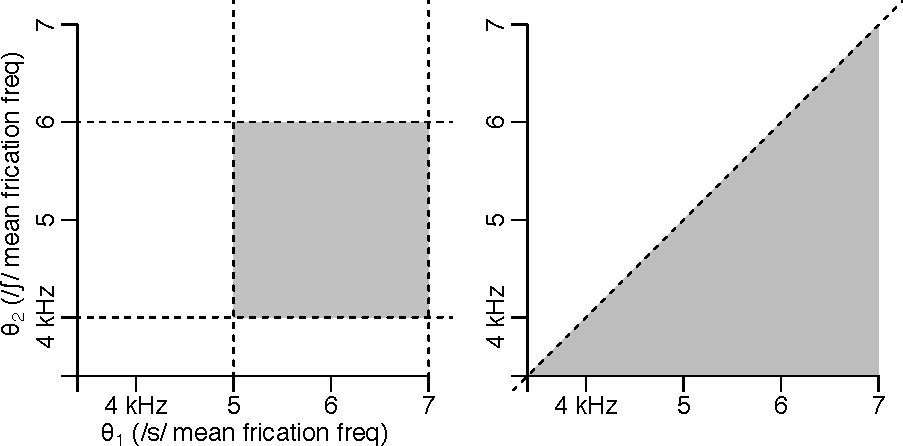
\includegraphics[width=0.5\textwidth]{part2-schematics/range-constraints-apart.pdf}
  \caption{Two examples of how prior experience with many talkers of a language can constrain the space of generative models that has to be searched during adaptation.  Left: an individual talker's mean frication frequency for \ph s generally falls in the \SIrange{5}{7}{\kilo\hertz} range, while the mean for \ph S is typically in the \SIrange{4}{6}{\kilo\hertz} range.  Combined, these exclude much of the logically possible space of generative models.  Right: moreover, the mean for \ph s is generally higher than the mean for \ph S, which also excludes a substantial proportion of the possible generative models.}
  \label{fig:range-order-constraints}
\end{figure}

An obvious question is where this belief updating process \emph{starts} for a novel talker. In the language of the ideal adapter, what are the listener's prior beliefs when first encountering an unfamiliar talker?  Before hearing any of a novel talker's speech, the only thing that the listener has to go on is their previous experience with \emph{other} talkers.  To the extent that there's structure to this experience that can benefit adaptation to a novel talker, it behooves the listener to take advantage of it, by \emph{generalizing} their experience with similar talkers.  At the highest level, all talkers of the same language are by definition similar, and thus one way in which experience with different talkers can help listeners is that it provides some information about the overall range, or distribution, of generative models that exist in the world, and hence that the listener should be prepared to expect from new talkers in the future.  By picking up on the structure of previous experience in this way, listeners can get a head start in adapting to a new talker, because their previous experience can tell them that some types of generative models are overall more likely than others.  For instance, across talkers of American English, a particular talker's mean \ph s frication frequency centroid (an important cue in distinguishing fricatives) generally falls in the range of \SIrange{5}{7}{\kilo\hertz}, and the mean \ph S frication centroid typically falls in the range of \SIrange{4}{6}{\kilo\hertz} \cite{Newman2001}.  This means that a listener can (probabilistically) rule out generative models where \ph s or \ph S have mean frication centroid outside these ranges, which substantially narrows down the range of generative models that they have to initially consider, providing a head start to adaptation (Figure~\ref{fig:range-order-constraints}).  There are further regularities at more specific ways of grouping talkers.  For instance, female talkers tend to produce both \ph s and \ph S with relatively high frication frequencies, while males tend to produce them with relatively low frequencies.  Thus, knowing something about indexical variables---who is talking, and what kind of person they are---makes some of the variability in generative models predictable.

Moreover, there are regularities across talkers in the relationships \emph{between} generative model parameters that a listener can take advantage of to give a further head start to adaptation.  For instance, even though the range of mean centroids for \ph s and \ph S overlap across talkers, \emph{within} a talker the mean centroid frequency for \ph s is almost always higher than for \ph S \cite{Newman2001}.  Based on this information listeners can also (again probabilistically) rule out generative models where the relative mean centroid of \ph s and \ph S is reversed from the typical pattern.  This sort of structure essentially cuts in half the number of generative models that need to be considered, a priori (Figure~\ref{fig:range-order-constraints}).  

Constraints like these make the problem of adapting to a new talker, in principle, vastly easier than learning the language in the first place.  The overall space of generative models that are likely to occur for a particular language or group of talkers is much more restricted than the space of generative models that occur across \emph{all} talkers of all languages.  Some of these constraints might be innate (and common, at least probabilistically, to the world's languages), but other obviously have to be learned for each particular language \cite<like the range of mean VOTs allowed for each category>{Lisker1964}.

\subsection{What do we know about how listeners generalize across talkers?}
\label{sec:what-do-we-know-gen}

\subsubsection{Generalizing across all talkers}
\label{sec:gener-across-all}

First, there is some tentative evidence that listeners are sensitive to the overall range of generative model they have encountered.  If listeners are sensitive to this range, then listeners who have experience with a broader range of generative models should, on average, be better prepared to adapt to unusual speech. \citeA{Baese-berk2013} found that, as predicted, listeners who had to transcribe sentences from four talkers with four \emph{different} foreign accents were more accurate on a fifth talker, with a fifth accent, relative to listeners who only heard a single accent (distinct from the test talker's).  

Conversely, listeners also use the range of generative models they have previously encountered to narrow down the hypotheses they consider for a new talker.  It follows that it should be \emph{harder} to adapt to talkers whose generative models fall outside the typical range.  This prediction is borne out in recent work.  For instance, \citeA{Idemaru2011} exposed listeners to various combinations of two cues to a voicing contrast (e.g. \ph b vs. \ph p), VOT and fundamental frequency (f0).  Canonically, these two cues are positively correlated within a talker: higher VOTs occur with higher f0s, and correspond to voiceless stops like \ph p. While uncorrelated VOT and f0 are rarer, they are also observed. Crucially, anti-correlated VOT and f0 are generally \emph{not} observed. If listeners have implicit beliefs that reflect these correlations, this should make it harder to adapt to unnatural talkers for which the two cues are anti-correlated. This is indeed what \citeA{Idemaru2011} found: listeners were able to adapt to a two-dimensional distribution of VOT and f0 where f0 was uncorrelated with VOT.  However, listeners were not able to fully adapt to a distribution where VOT and f0 were anti-correlated. Similarly, \citeA{Sumner2011} found that American English listeners were not able to adapt to a talker who always produced voiced stops (i.e. \ph b, \ph d, \ph g) with substantial prevoicing (negative VOTs).  Given that American English talkers typically produce these sounds with VOTs of \SI{0}{\milli\second}, this inability to adapt, too, might be a consequence of cross-talker generalizations based on prior beliefs. 


\subsubsection{Generalizing based on social group membership}
\label{sec:soci-group-memb}

Listeners often know (or can infer) more about a talker than that they are a speaker of English (or whichever language).  To the extent that different a particular group of talkers systematically differs in their generative models from talkers in general, the listener can benefit by identifying whether a talker is a member of this group, and using their previous experience with this group to provide an even bigger head start to adaptation.  For instance, there are dramatic differences in how men and women produce many phonetic categories \cite<e.g.,>{Hillenbrand1995,Jongman2000,McMurray2011a,Newman2001}, and thus the listener might (probabilistically) rule out a range possible generative models, further facilitating fast adaptation.\footnote{Of course, as above, if the talker's generative model is actually outside the normal range for women, this would \emph{hurt} adaptation.  But, by definition, the distribution of the generative models for talkers in a particular group captures most of the talkers in that group, and so \emph{on average} will be beneficial.}  

One straightforward prediction of this is that in the absence of enough direct experience with a talker to directly converge on that talker's generative model, the listener's beliefs will be a combination of their (gender-specific) prior beliefs and whatever they manage to glean from what speech they have observed.  For speech sounds that differ systematically between male and female talkers, such as fricatives, the listener's best guess about the appropriate generative model for the current speech is expected to depend on whether the listener believes the signal to stem from a male or a female talker.  If, as we have argued above, listeners use these beliefs about the generative model to guide interpretation of speech sounds, then changing the perceived gender of the talker should change categorization (e.g., by displaying a picture of a male vs. female face along with the audio stimulus) .

This prediction is born out in a study by \textcite{Strand1996} \autocite[see also][]{Strand1999,Munson2011a}.  Listeners heard sounds on an \ph s-\ph S (``sod''-``shod'') continuum, made by varying the frication frequency from high (\ph s-like) to low (\ph S-like), paired with either a male or a female face.  Frication frequencies are typically lower overall for male talkers than for female talkers \cite{Jongman2000,McMurray2011a,Newman2001},  If listeners take this information into account then they should place the \ph s-\ph S boundary at a \emph{higher} frequency if they think the talker is female, resulting in \emph{fewer} \ph s responses.  This was exactly what \citeA{Strand1996} found.  Analogous results have been found using vowels \cite{Johnson1999} and using different vocal sources as cues to gender \cite<rather than faces>{Strand1996,Strand1999,Johnson1999,Munson2011a}.  

Beyond gender, there is evidence that listeners also use their experience with the speech of different social groups as a source of information about where to start adaptation.  In a vowel matching task where they were told that the talker was from Canada, listeners from Detroit, MI chose tokens with more Canadian raising as matching than when they were told the talker was from Detroit \cite{Niedzielski1999}.  This suggests that listeners' perception of these vowels was biased towards what they expected to hear from a Canadian talker.  There is, more generally, a growing literature on the extent to which perceived social group membership affects language comprehension \autocite{Drager2010,Hay2006,Hay2010,StaumCasasanto2008,Sidaras2014}.

\subsection{How does the ideal adapter formalize generalization across talkers?}
\label{sec:how-ideal-adapter-gen}

\begin{figure}[htb]
  \centering
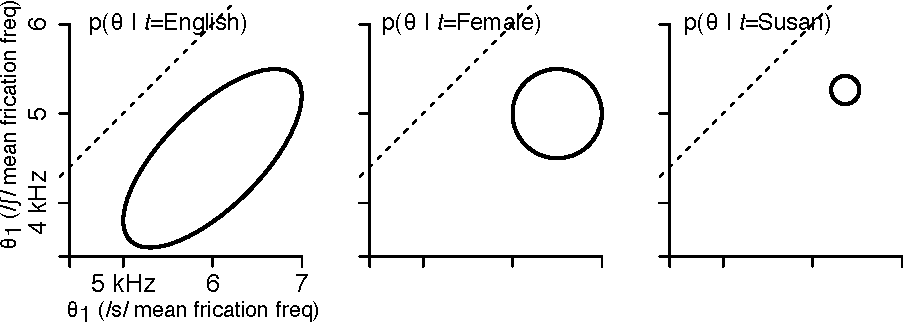
\includegraphics[width=0.75\textwidth]{part2-schematics/english-male-talker-annotated.pdf}
  \caption{Prior beliefs at varying levels of specificity, formalized as conditional distributions over generative model parameters (plotted as ellipses of most probability mass).  Left: Experience with all talkers of English constrains the listener's prior beliefs about another talker of English, but only very broadly: the mean frication centroid for \ph s tends to be higher than for \ph S, and they tend to be positively correlated, but the actual values can range quite a bit. Middle: experience with all female talkers provides more information, because female talkers tend to pronounce \ph s and \ph S with frication frequency means on the high side of the overall range. Thus the distribution of females' generative model parameters for \ph s and \ph S is more concentrated than that of all English speakers. Right: experience with a particular female talker provides even more information, and the corresponding distribution over generative model parameters is even more concentrated}
  \label{fig:prior-beliefs-different-scales}
\end{figure}

In the ideal adapter framework, the listener's beliefs about generative models are formalized as distributions over generative models, which assign more or less probability to each possible generative model.  This is true both for beliefs about a particular talker's or situation's generative model, like $p(\theta \given \mathrm{Susan})$. We can also formalize beliefs about what generative models are likely for any talker of the language---$p(\theta \given \mathrm{English})$---or for a female talker---$p(\theta \given \mathrm{female})$---or a Canadian talker---$p(\theta \given \mathrm{Canadian})$.  When first encountering a novel talker, all the listener has to go on are these sort of beliefs about the distribution of generative models \emph{across} individual talkers in some group.  

Above, we have talked intuitively about how the listener's experience with the generative models of different talkers from a novel talker's language or social group can rule out a lot of generative models ahead of time and give a head start to adaptation.  In the ideal adapter framework, this is a consequence of thinking about belief-updating as statistical inference, where the distributions over generative models corresponding to the listener's prior beliefs and the information from the speech they observe are combined according to Bayes rule.  In order to converge on the particular generative model for the current situation, the listener has to allocate more and more probability mass to it.  Consequently, the more probability is allocated to it ahead of time, the less information is required from observations.  

The reason that more specific (or constraining) prior beliefs provide more of a head start is that by definition, probability distributions have to add up to one, and so spreading probability mass over a larger range of generative models means that less probability mass is allocated to each \emph{particular} possible generative model.  Thus, conversely, the more generative models that the listener can exclude a priori, the more probability they can allocate to each remaining generative model.  If the actual generative model for the situation lies within this range, then fewer consistent observations are required in order to reach a particular level of probability for the actual current generative model.  

The price that is paid for this head start is that more specific prior beliefs are less \emph{flexible}.  That is, if the prior beliefs are \emph{wrong} and the actual generative model lies outside the range that has non-trivial  prior probability, then much more evidence will be required to reach the same level of belief in the actual generative model.\footnote{This is really a consequence of Bayes rule assigning posterior probability as the \emph{product} of prior probability and likelihood.  That means that what ``adds up'' is actually \emph{log}-probability, which goes to negative-infinity as probability goes to zero.}  This is why, in principle, the listener should only use specific beliefs when they are fairly certain that they are applicable.  While this might seem like a problem for the ideal adapter framework, in the next section we will show that the ideal adapter framework also points towards a solution, which is to treat the problem of identifying which beliefs are applicable as another inference problem, which can be solved by combining top-down information (like visual recognition of a particular talker) with bottom-up information from the speech itself.

\subsection{Open questions: Generalization across talkers }
\label{sec:open-questions-gen}
\label{r1-gen-questions}

\subsubsection{How do listeners know who to group together?}
\label{sec:how-do-listeners}

In order to make use of structure in the distribution of generative models at different levels---from talker-specific to groups of talkers to the overall base distribution---listeners have to somehow pick up on and \emph{learn} this structure.  There is some evidence that people can not only induce this sort of structure, but in some cases can do so surprisingly quickly.  \citeA{Bradlow2008} had listeners transcribe sentences from accented talkers.  In the \emph{same talker} condition, the sentences were all produced by a single accented talker, and listeners transcribed sentences from this same talker more accurately in a later test phase.  In the \emph{multiple talker} condition, listeners transcribed the same total amount of speech, but from four different talkers (distinct from the test talker).  Despite the test talker being novel to them, listeners in the multiple talker condition showed the same benefit of experience as the same talker group.  Listeners in a \emph{single other talker} condition did not receive any benefit to exposure to a single accented talker when tested on the novel test talker, which suggests that listeners in the multiple talker condition have extracted some accent-level beliefs after a relatively small amount of exposure (on the order of an hour or two).

In the language of the ideal adapter framework, we might say that listeners need to impute structure to the variability in the generative models they have experienced.  Much like Bayesian models of category learning during language acquisition \cite<e.g.>{Feldman2013a,Perfors2011}, this structure induction can be thought of as another problem of inference under uncertainty.  Each way of grouping previously encountered generative models is an imputation of some kind of structure, and each possible grouping may be more or less compatible with previous experience and a priori expectations about how likely particular sorts of groupings are.  However, the ideal adapter framework, as articulated here, has very little specific to say about how this inference might work---even at a computational level---outside of very general predictions \autocites[e.g. simpler groupings are naturally preferred because of the Occam's razor property of Bayesian inference;][]{Perfors2011}[pp. 343-356]{Mackay2003}.

\subsubsection{How are multiple, overlapping groups represented?}
\label{sec:what-repr-are}

\label{r1-features-classes}
Each individual talker can belong to many different groups of talkers, all of which may be informative about their generative model.  There are many ways that such a structure might be represented formally.  One of the simplest possibilities is that talkers are nested within groups (``Mandarin-accented male talkers''), which are themselves nested within more general groups (``Mandarin-accented talkers''), and so on.  This has the potentially problematic feature of not allowing generalization to a combination of groups that has not directly been observed.  Another possibility is that groups might be represented, not as absolute generative model parameter distributions, but as offsets from the parameters predicted based on other factors (including other group memberships).\footnote{For an analogous model applied to allophonic variation of phonetic categories, see \citeA{Dillon2013}.}  This would make it possible to generalize based on arbitrary combinations of features, without needing direct experience with a particular combination, but at the price of requiring the same offset for, say, male vs. female talkers regardless of their other group memberships.  

These possibilities lead to at least two open questions. First, do listeners, in fact, generalize from experience with a male talker with a particular accent or dialect to a female talker of the same accent or dialect (and vice-versa)?  If listeners can generalize within a gender but not across, this would suggest that they have beliefs that are specific to a particular combination of gender, dialect/accent, and possibly other indexical variables.  Of course, it is possible that for \emph{some} dialects/accents listeners have gender-specific beliefs, while for others they do not.  This leads to the second question: do males and females differ in the same way across all dialects/accents of a language?  If the ways that the generative models depend on these different types of indexical variables are all independent of each other, then it makes sense to separate them out into orthogonal features.  However, gender differences themselves vary quite a bit across languages \cite{Johnson2006}, so it is not implausible that within a language there might be dialectal variation in gender differences as well.  Moreover, it is altogether possible that for some groups, gender has the same (independent effect) while for others it does not.  If this is the case, then it is in those kinds of groups where gender has an independent effect that the ideal adapter predicts that listeners are most likely to generalize experience across genders. The advent of the widespread availability and use of speech recognition technology presents an exciting opportunity to gather speech from large samples of individuals, potentially allowing some of these questions about the distribution of generative models in the world to be addressed.

\label{r1-gen-questions-end}

\section{Balancing stability and flexibility: When to adapt, generalize, or recognize}
\label{sec:when-adapt-gener}

Thus far, we've addressed three strategies that listeners have for dealing with the lack of invariance: rapid adaptation to totally novel talkers, recognition of familiar talkers (and the resulting talker-specificity), and generalization across groups of similar talkers.  In the ideal adapter framework, all three of these strategies are the result of the listener trying to infer the appropriate generative model with differing degrees of relevant prior experience.  In this way of thinking, whether speech perception is flexible---as in adaptation to novel situations---or stable---as in recognition of familiar situations---depends on how confident the listener is in their prior beliefs, which in turn depends on how much relevant prior experience they have. 
In order to introduce the relationship between these strategies and the type and amount of relevant prior experience the listener has, we have so far addressed these strategies separately, assuming in each case that the listener \emph{knows}---based on non-linguistic cues---what kind of prior experience is relevant to the current situation.

While such cues are often available, they are not \emph{always} available, and sometimes they do not provide high certainty. Consider, for example, the case of running into someone that one remembers from somewhere but doesn't quite remember who it is. Sometimes visual or other cues are absent, such as when picking up the phone in the absence of caller ID, or listening to a conference call with many different people.  In these cases where there is some uncertainty about \emph{who} is talking, there is also uncertainty about what prior experience will be most helpful in figuring out that talker's generative model (and ultimately what they are trying to communicate).  When top-down cues do not unambiguously identify the talker (or type of talker), the listener can still benefit from prior experience. Specifically, if the listener can identify a familiar talker (or the group that a talker belongs to) from their speech, listeners will have nearly the same benefits of prior experience as if they had known the talker's identity ahead of time.

The ideal adapter treats the problem of whether to be flexible or stable as inference under uncertainty at yet a third level, where the listener tries to infer what \emph{type} of situation they are in, and hence what prior experience will be relevant in figuring out the generative model.\footnote{The other two levels being inferring the intended category, and inferring the situation's particular generative model.}  There are, as always, two sources of information that can guide this inference: the listener's top-down expectations about what type of situation they are in (like visually identifying a talker's face), and bottom-up information from the speech signal (which may be more or less compatible with the speech predicted by their beliefs about each possible type of situation).  The ideal adapter framework predicts that listeners use these two sources of evidence in order to balance stability and flexibility on the fly.

\subsection{What do we know about how listeners balance stability and flexibility?}
\label{sec:what-do-we}

Balancing stability and plasticity requires that listeners deploy the most informative prior experience that is relevant in each situation.  This is true whether or not they know \emph{a priori} what prior experience is relevant.  Thus, we argue, balancing stability and plasticity in speech perception requires that the listener dynamically combine top-down information about what kind of situation they are in with bottom-up information from the speech signal.  However, little is known about how listeners trade off these two sources of information.  What little we know suggests that listener do, in fact, use both bottom-up and top-down information to infer the type of situation they are in and what prior experience is currently relevant. Based on these inferences, listeners can then determine how flexible to be in the current situation. Evidence for this view is of two types, which we discuss in turn.  First, listeners can recognize talkers that they are familiar with based on just bottom-up speech input.  Second, listeners generalize experience with one talker to adaptation to another talker based both on the bottom-up similarity in their generative models and top-down expectations that generalization is appropriate.  

\subsubsection{Recognizing familiar talkers based on their speech}
\label{sec:recogn-famil-talk-1}

Listeners use information from the speech signal itself to help infer the talker's identity (and social group membership) in a way that shapes how they interpret that talker's speech.  The speech signal includes non-phonetic features like (in English) f0 range, jitter, and shimmer that distinguishes talkers \cite{Creel2011,Pardo2006}.  Listeners use this information not only to recognize familiar individuals but also to infer social group membership.  For instance, we discussed above evidence that listeners change their classification of vowels and fricatives based on the gender of a visually presented face.  These same studies found that synthesized vowels and fricatives---with exactly the same phonetic cue values---were also classified differently depending on the vocal source wave that was used, with stereotypically female and male vocal sources having a similar effect as a visually-presented female face (higher frequency category boundaries).  Interestingly, this effect is gradient, with the effects of voices rated as non-stereotypically male or female falling in between stereotypically male or female voices \cite{Johnson1999,Munson2011a,Strand1996,Strand1999}.

Beyond non-phonetic aspects of the speech signal, the fact that different talkers use different phonetic generative models means that \emph{phonetic} aspects of the speech signal can also, in principle, provide information about talker identity or group.  That is, the same talker- or group-specific beliefs about the phonetic generative model which benefit speech perception once a particular talker is identified can \emph{also} conversely aid in identifying a talker.  To the extent that they vary across talkers---and hence benefit from talker- or group-specific representations---phonetic features like formant frequencies and VOT are by definition diagnostic of talker identity.  Thus, the listener's knowledge about a familiar talker's cue statistics provides a rich source of information for identifying that particular talker based on their speech, which can in turn can affect how that same speech signal is mapped onto phonetic categories.  Listeners do, in fact, take advantage of such phonetic information for talker recognition \cite{Creel2011,Pardo2006}, and can explicitly recognize talkers with very high accuracy based on sine-wave \cite{Remez1997} or noise vocoded speech \cite{Sheffert2002}.  Such processing of speech removes all of the fine spectral detail (and much if not all of the voice quality information) but preserves enough phonetic information to allow for reasonably good comprehension.

\subsubsection{Generalizing experience with one talker to another, or not}
\label{sec:recogn-novel-talk}

When there is uncertainty about what prior experience is relevant, information from the speech signal helps processing of novel talkers in two ways.  First, in this paper we have generally simplified our discussion by focusing on a few phonetic features.  However, in everyday speech perception the generative model is highly complex, covering many categories, each cued by many acoustic features.  Somewhat paradoxically, when we consider that the listener must also infer the kind of prior experience that is relevant, this makes their job easier: even from a small amount of speech from a novel talker, listeners can in all likelihood recognize that none of their talker-specific representations provide a good match to the current situation.  Second, even a small amount of information about the generative model can help identify whether, and which, more informative \emph{group}-specific beliefs might be relevant, meaning that listeners have to fall back on the least informative beliefs only as a last resort.  This is important because on the one hand, even a little bit of experience with one or more similar talkers provides a big boost to adaptation, but on the other hand, mistakenly assigning a talker to a particular group actually makes it harder to adapt to their actual generative model, as discussed in the last section.  If listeners are in fact continuously trying to identify what, if any, familiar group a novel talker belongs to based on the speech they produce, then they should flexibly generalize from experience with one talker to another when it's warranted (by top-down expectations and bottom-up similarity) but adapt in a talker-specific way when it is not.

This is an important though comparatively understudied issue.  A series of recent studies provides some tentative evidence for the predictions of the ideal adapter framework.  These studies looked at how much listeners generalize perceptual learning for a male talker to a different, female talker \cite<or vice versa;>{Eisner2005,Kraljic2005,Kraljic2006,Kraljic2007}.  In one version of these experiments listeners hear a male talker's production of a sound ambiguous between a \ph s and a \ph S, embedded in a word that indicates it was intended to be an \ph s.  After exposure, listeners are tested on two different \ph s-\ph S continua: one produced by the same male talker as exposure, and the other produced by a different (female) talker.  In the case of \ph s-\ph S (and \ph s-\ph f), listeners show the expected recalibration effect---more \ph s responses after \ph s exposure---when tested on the same talker, but no effect when tested on the different, female talker \cite{Eisner2005,Kraljic2005}.  However, in another version of the experiment using a \ph d-\ph t contrast, listeners show the same recalibration effect on \emph{both} the same- and different-talker test continua \cite{Kraljic2006}.  In such experiments, the only information that the listener has about the unfamiliar female test talker comes from the test stimuli themselves.  In the case of a voicing contrast like \ph d-\ph t, the overall distribution of the critical cue---VOT---is generally similar between the familiar male and unfamiliar female talker, and so the test stimuli provide information that these two talkers' generative models are overall quite similar, at least in terms of VOT and the voicing contrasts it cues.  If listeners are using this information, then they should apply what they have learned about the male talker to the unfamiliar female talker, which would lead to the generalization observed by \citeA{Kraljic2006}.  Conversely, the range of cues in the \ph s-\ph S male and female continua used by \citeA{Kraljic2005} differ quite dramatically: the highest spectral centroid of the male talker's \ph s is still lower than the \emph{lowest} \ph S end of the female talker's continuum.  Thus, the test stimuli from the female test talker provide evidence that these two talkers are quite different in how they produce this contrast, and thus it does not make sense to apply what has been learned about the male talker to the unfamiliar female test talker.  

\citeA{Kraljic2007} present evidence that listeners use both their top-down expectations about whether two talkers should be grouped and the bottom-up similarity of their cue statistics to guide not just processing of a totally unfamiliar test talker, but also to guide adaptation to multiple talkers.  When exposed to both a male and female talker, whose ambiguous pronunciations are disambiguated in opposite ways (e.g. male as \ph d and female as \ph t), listeners showed no overall learning effect between pre- and post-exposure classification of the two talker's \ph d-\ph t continua, suggesting that they have tracked the statistics of these categories in a talker-independent way.  But for the analogous procedure with \ph s-\ph S, classification of each talker's continuum shifted in the typical way, suggesting that they have adapted talker-specific representations \cite{Kraljic2007}.  

This might be taken as evidence that listeners are simply unable or categorically unwilling to learn and maintain talker-specific beliefs about some phonetic categories.  This broadly makes sense: for categories like \ph d versus \ph t which, in the listener's experience, show some variability across talkers but are not systematically produced differently by male versus female talkers, it is a reasonable guess that a male and a female talker encountered in the same context will produce them similarly and can be grouped together.  Likewise, as noted by \citeA{Kraljic2007}, for categories that are generally produced differently by male and female talkers who are otherwise similar, it is a good bet that a male and female talker should \emph{not} be grouped together.

However, if listeners are actually trying to \emph{infer} whether or not two talkers should be grouped together---rather than simply relying on fixed heuristics---then enough of the right kind of experience which contradicts these biases should be able to overcome them in specific cases.  For instance, even though listeners tend to generalize experience with VOT distributions from a male to female talker, with sufficient experience with a male and a female talker who have \emph{different} VOT distributions, listeners do in fact learn talker-specific representations \cite{Munson2011}.  Conversely, even though listeners tend to learn talker-specific representations of fricatives, by using a modified test continuum \citeA{Reinisch2014} found that listeners can generalize experience with a female talker's fricatives to a novel male talker.
\label{r1-reinisch1}

\subsection{How does the ideal adapter formalize the stability/plasticity trade-off?}
\label{sec:how-does-ideal}

\subsubsection{A mixture of prior beliefs}
\label{sec:mixt-prior-beli}

The available evidence suggests that listeners can, on the fly, infer which type of prior experience is relevant for the current situation based on a combination of bottom-up speech information and top-down expectations.  In the language of the ideal adapter framework, this in turn suggests that in situations where the listener is unsure about what type of prior experience is relevant, their prior expectations about what generative models they will encounter are a \emph{mixture} of expectations given different types of prior experience.  Each particular sort of prior experience can be thought of as a cluster of possible generative models, with more specific prior experience---like experience with a particular familiar talker---corresponding to highly concentrated, peaked clusters and more general experience---like with the range of generative models across all talkers in the language---being more spread out.  
How much each cluster contributes to the overall beliefs depends on how likely the listener thinks it is to apply in the current situation.  How much the listener expects to encounter any \emph{particular} generative model is thus a combination of how much it is expected given a particular set of beliefs, and how likely the listener thinks those beliefs are to apply.  


One way to formalize this notion is based on representing the beliefs about generative models for a particular type of prior experience as a probability distribution over generative models.  Again, for the sake of brevity, we refer to the generative model by its parameters\footnotemark[\ref{note:gen-mod-params}] $\theta$, conditional on the \emph{type} of prior experience $t$: $p(\theta\given t)$.  Here, we use $t$ to denote a more general form of talker identity, that covers beliefs ranging from particular individual talkers, like $p(\theta \given t=\mathrm{my\ father})$, to groups, like $p(\theta \given t=\textrm{Boston accent})$, all the way to language-level groupings like $p(\theta \given t=\textrm{English speaker})$.  Above, we assumed that the listeners \emph{knows} the type of prior experience which is relevant, and thus only a single conditional distribution $p(\theta \given t)$ is relevant.  When the listener is uncertain, though, multiple different conditional distributions might be relevant.  The listener's beliefs about which type of prior experience is relevant can be formalized as a probability distribution over the types $t$---$p(t)$---and hence their overall beliefs about the generative model parameters as a \emph{mixture} of the conditional beliefs, weighted by $p(t)$: 
\begin{equation}
  \label{eq:30}
  p(\theta) = \sum_t p(\theta \given t) p(t)
\end{equation}

\subsubsection{Top-down information}
\label{sec:top-down-information}

Let's consider the case where the listener can recognize a familiar talker---call him Frank---with high certainty based on visual information.  Then, the distribution over types of prior experience $p(t \given \textrm{vis. info})$ is highly peaked:
\begin{equation}
  \label{eq:31}
  p(t \given \textrm{vis. info}) = \left \{
    \begin{array}{rl}
      1 & \textrm{if } t=\mathrm{Frank} \\
      0 & \mathrm{otherwise}
    \end{array}
  \right .
\end{equation}
As a result, the listeners' beliefs about the generative model parameters, given the visual information that identifies the talker as Frank, is dominated by their beliefs about Frank's generative model: 
\begin{align}
  \label{eq:32}
  p(\theta \given \textrm{vis. info}) &= \sum_t p(\theta \given t) p(t \given \textrm{vis. info}) \\
  &=p(\theta \given t=\mathrm{Frank}) p(t=\mathrm{Frank} \given \textrm{vis. info}) + \sum_{t \ne \mathrm{Frank}} p(\theta \given t) p(t \given \textrm{vis. info}) \\
  &= p(\theta \given t=\mathrm{Frank}) \times 1 + \sum_{t \ne \mathrm{Frank}} p(\theta \given t) \times 0 \\
  &= p(\theta \given t=\mathrm{Frank})
\end{align}

That is, when the type of prior experience is known with reasonably high certainty from top-down cues, this mixture model reduces to the talker- or group-specific beliefs described in earlier sections in Part II.  This formalization thus generalizes the notion of talker- or group-specific beliefs as conditional distributions.  In this sort of mixture model, when top-down information about the type of situation is available, listeners can take advantage of it, which can in turn lead to effects of top-down information (like visually presented faces or other cues) changing the way that physically identical bottom-up acoustic signals are interpreted \cite{Johnson1999,Hay2010,StaumCasasanto2008,Strand1996}.  However, having a weighted mixture of different prior beliefs means that the listener does not have to rely \emph{solely} on such top-down information to tell them which prior experience is relevant, but rather can also use bottom-up information.

\subsubsection{Bottom-up information}
\label{sec:bott-up-inform}

Formalizing the listener's prior beliefs about generative models in this way provides a natural way of formalizing how bottom-up, phonetic information can help infer the type of prior experience that is relevant.  Inferring the type of experience that is relevant comes down to inferring the type $t$, given some observations $x$ and prior expectations $p(t)$, which we can think of as Bayesian inference at yet another level: 
\begin{equation}
  \label{eq:33}
  p(t \given x) \propto p(x \given t) p(t)
\end{equation}
As usual, the listener's updated beliefs about the type of situation they are in, $t$, are a combination of their prior beliefs about the type of situation $p(t)$, and how well their prior experience with each type predicts the observations $x$, $p(x\given t)$.  In this formalization, observations and types are assumed to be only indirectly related, via the generative model parameters $\theta$: each type predicts a range of generative models, $p(\theta \given t)$, and each value of the generative model parameters predicts a range of observations, $p(x \given \theta)$.  In order to get the \emph{marginal} likelihood of the signal $x$ under situation $t$, $p(x\given t)$, the particular values of the generative model parameters have to be averaged out:
\begin{equation}
  \label{eq:34}
  p(x \given t) = \int p(x \given \theta) p(\theta \given t) \ud \theta
\end{equation}

The jargony term for this averaging is \emph{marginalization}. And a natural consequence of marginalization is that it leads to a preference for the most specific prior experience which provides a reasonably good fit to the observed data.  We can think of marginalization as essentially taking a weighted average of the likelihood of the observation $x$, $p(x \given \theta)$, weighted by the type-specific probability of the generative model parameters $p(\theta \given t)$.  On the one hand, for a type of prior experience that leads to very specific beliefs---like a particular familiar talker---the predicted observations $p(x\given \theta)$ are very similar over the range of generative models that are given reasonably high probability, and so will all either fit the data reasonably well or not.  On the other hand, a type of prior experience that leads to less specific beliefs about generative models---like experience with all speakers of the language---predicts a lot of different generative models.  Some of these will probably provide a good account of the observation $x$---high likelihood $p(x \given \theta)$---but the vast majority will not, resulting in a low average (maringal) likelihood $p(x \given t)$. 

This trade-off between specificity and accuracy goes both ways.  A vague (e.g. language-wide) prior over generative models will allocate \emph{some} likelihood to nearly \emph{any} observation, whereas a specific (e.g. familiar talker) prior predicts only a very limited range of observations, and so assigns very high marginal likelihood to things in that range and basically nothing outside of it.  So for observations that fall outside the range predicted by previous experience with specific talkers, less specific, group-level experience provide the best marginal likelihood, even if it's not (in absolute terms) very high.  

Of course, inferring the type of prior experience that is relevant is only the first step to robust speech perception.  Additionally, the listener also needs to infer the generative model that is best suited to the current situation.  We can think of this as inference of the \emph{joint posterior} distribution of generative model parameters and type of situation, $p(\theta, t \given x)$.  This combines inference about the type of situation---as discussed in this section---with situation-specific belief-updating---discussed above: 
\begin{equation}
  \label{eq:36}
  p(\theta, t \given x) = \underbrace{p(\theta \given x, t)}_{\substack{\textrm{situation-specific}\\\textrm{updated beliefs}}} \underbrace{p(t \given x)}_{\substack{\textrm{type of}\\\textrm{situation}}}
\end{equation}
Alternatively, we can think of just the overall updated beliefs about the generative model $p(\theta\given x)$, which---like the prior beliefs $p(\theta)$---are a mixture of updated situation-specific beliefs, weighted by how likely each situation is given the observation: 
\begin{equation}
  \label{eq:37}
  p(\theta \given x) = \sum_t p(\theta, t \given x) = \sum_t p(\theta \given x, t) p(t \given x)
\end{equation}

This brings us back to the central point of the second part of this paper: 
the ideal adapter framework reveals that we can look at recognition (and the resulting talker-specificity), adaptation, and generalization in speech perception as the natural consequence of a system that is trying to do the best that it can to comprehend speech in a variable---but structured---world.  Because of the variability (or subjective non-stationarity) of the statistics of the speech signal, the listener has to adjust the generative model they use.  There are two sources of information that listeners have when trying to do this: the speech they are currently processing, and their previous experience and prior expectations.  Different strategies arise from the fact that in each situation, the prior experience that is relevant---if any---is sometimes more and sometimes less informative about the appropriate generative model than the current speech itself.  When the listener has no relevant prior experience, the best they can do is to try to learn the generative model by adapting their beliefs to better match the recently observed speech statistics, leading to rapid adaptation.  When they have prior experience that is \emph{directly} relevant, like with a familiar individual talker, the best thing they can do is to rely on that prior experience, removing the need to adapt and leading to talker-specific speech perception.  When they have experience that is relevant, but not directly, then the best they can do is apply that experience to the current situation and then use the actual speech statistics to converge on an appropriate generative model.
 
For types of experience that correspond to very specific beliefs---like a highly familiar talker---the situation-specific beliefs will change little with the addition of one more observation.  If such a component for a familiar talker provides the best match to the observed speech, then the result of this process of belief updating with a clustered mixture prior is that the listener has recognized and deployed their talker-specific generative model.  If, on the other hand, the best-fitting type is a very broad, general type like all speakers of English, then the updated beliefs are dominated much more by the actual observed data then the prior, just like when the listener knows ahead of time that they need to adapt rapidly.  Similarly, if prior beliefs of intermediate specificity dominate, then the updated beliefs will reflect the observed data more than they would for a highly familiar talker, but the prior beliefs will contribute more than in the most flexible case.   This is how the ideal adapter is able to flexibly deal with the lack of invariance, making the best use of different types of prior experience with different generative models.  By learning about and representing the \emph{distribution} of generative models in the world, the ideal adapter is better prepared to infer the appropriate generative model across many different types of situations.  


\subsection{Open questions}
\label{sec:open-questions-infer-cluster}
\label{r1-cluster-questions}

We have argued here that the ideal adapter predicts that listeners dynamically balance flexibility and stability by \emph{inferring} what kind of prior experience is currently most relevant.  If the listener decides that experience with a particular familiar talker is most relevant, they will show stable, talker-specific speech perception.  If, on the other hand, they decide that the only relevant prior experience they have is with the full distribution of talkers of the language, then they will rapidly and flexibly adapt.  

The biggest open question that this raises is how---and even whether---listeners combine top-down and bottom-up information about what kind of prior experience is relevant.  There are, in our view, at least two sides to this question.  The first side is what a truly ideal adapter would do.  The ideal adapter framework as currently posed addresses this only in the most general sense, saying that listeners \emph{should} combine top-down and bottom-up information to determine what prior beliefs to use.  But much more work is required in order to make further testable predictions.  The second side is empirical, and in the rest of this section we review two empirical questions we see as particularly pressing.

\subsubsection{What role do expectations of generalizability play?}
\label{sec:what-role-expect}

The studies by \citeA{Kraljic2005,Kraljic2006,Kraljic2007} suggest that listeners group together talkers when the distributions of cues they produce are similar.  But in all these studies, the similarity of the cue distributions is confounded with the overall similarity between male and female talkers in general on the relevant phonetic dimensions: male and female talkers don't systematically differ in their VOT distributions in American English \cite{Allen2003}, whereas they do differ in their frication frequency distributions \cite{Newman2001}.  Thus listeners may have already made up their minds about whether to group the two talkers together before hearing anything.  There's some evidence that top-down expectations and bottom-up similarity can be dissociated \cite{Munson2011,Reinisch2014}, but it remains to be seen exactly how listeners balance these two sources of information, both in the short term (e.g. over the course of a single experimental session) and over the long term (over days, weeks, or longer).
\label{r1-reinisch2}

\subsubsection{When are two generative models similar enough to group?}
\label{sec:open-questions}

Our discussion of how listeners might generalize experience from one talker to another on the basis of similarity of their generative models glosses over a very basic point: even if their VOT ranges are overall very similar, the whole generative model for a male talker is \emph{very} different from that of a female talker.  Thus, while it might make sense to lump together experience with a male and female talker for the purposes of inferring their VOT distributions, it definitely does not make sense to lump together beliefs about their vowels.  One way that this dilemma could be resolved is if listeners have extracted some information about the variance of different parameters in groups that contain males and females (like the ad hoc grouping that might be inferred during an experiment).  Properties that vary a lot across talkers within a group are not very informative about particular talkers, whereas properties that are consistent across talkers in a group can be used to constrain beliefs about individuals much more strongly.  Because males and females---within most groups---vary a lot in their vowels, but not so much in their VOT, listeners can use information about the VOT distributions of individual talkers to (on average) reliably infer properties of the group, which in turn are (on average) highly informative about properties of other talkers in the same group.

An alternate possibility is that listeners have more or less separate beliefs about different ``chunks'' of the generative model, potentially grouping talkers differently when considering beliefs about their VOT distributions than they do when considering beliefs about vowel formants.  It is not immediately obvious what---if any---divergent predictions these two accounts would make, and more work is required to understand both their computational implications and related human behaviors.

\label{r1-cluster-questions-end}

\section{Part II conclusion}
\label{sec:part-ii-conclusion}

We have argued that a range of strategies that human listeners use to deal with the lack of invariance all correspond to the best that they can do in a world where generative models vary from one situation to the next, but do so in a structured way that is tied to indexical variables like talker identity and group membership.  The ideal adapter framework formalizes this notion by representing situation-specific beliefs about the range (distribution) of generative models that are expected in different types of situations, from very specific (an individual talker) to very general (an entire language).%
Although it is beyond the scope of this paper to discuss in any detail, this perspective can be applied to second (and third, etc.) language acquisition as well (\citeauthor{PajakSubmitted}, \emph{under review}).
This range allows the listener to balance stability and flexibility, relying on prior experience when it is available and relevant, falling back on less informative but more flexible group-level beliefs. This system is not fail-safe. In order to achieve robust recognition of familiar talkers and guiding generalization across talkers, the speech perception system is forced to rely on prior experience. In highly atypical situations --which, fortunately, are bound to be rare-- this very same property can slow down or prevent successful adaptation and perception (as also evident in second language learning). 

Explicit structured beliefs are one way of achieving sensitivity to structured variability of cue-category mappings. However, the primary take-home message from Part II is that sensitivity to this structured variability is a critical feature of any model that seeks to explain the robustness of human speech perception.  Formulating such a model and evaluating its predictions remains a task for future work.


\section*{Part III}
\label{sec:part-iii}

We close our paper with a discussion of how the present work relates to other approaches and issues.  We chose to take a \emph{computational-level} approach to understanding how the speech perception system deals with the lack of invariance. Such an analysis focuses on the \emph{problem} of robust speech perception. That is, our approach is guided by questions about the `why', or the purpose of the system, the goals it typically serves, and the world it has to function in.  Focusing on the `why' of speech perception does not  directly address the actual cognitive processes (and neural mechanisms) that must carry it out \cite{Marr1982}, but it has allowed the development of models that provide a good fit to human behavior, both in speech perception \cite{Clayards2008,Feldman2009a,Norris2008,Sonderegger2010} and in a range of phonetic adaptation phenomena (Part I of this paper).  It also has allowed us to make novel predictions, some of which we have tested here and the rest of which we hope will guide future research and the development of cognitive and neural models.  The ideal adapter framework is \emph{normative}, in that it looks only at the in-principle constraints on performance that come from the inherent difficulty of the task and the limited information that is available in the world, without considering resource limitations.  The brain is obviously not unbounded in its resources, and considerations that come from processes, representations, and mechanisms are thus relevant to future development of the framework presented here. 

However, this gulf is not as wide as it might first appear.  Neurally plausible algorithms exist for the sort of inferences required by the ideal adapter framework \cite{Beck2012a,Friston2005,Rao1999}, and resource limitations can be included in a normative framework. For instance, recent work has focused on developing ``rational approximations'' to rational (normative) models like the ideal adapter.  These models ask what the best possible performance is under different types and levels of cognitive or neural resource constraints \cite{Griffiths2012,Sanborn2010,Shi2010}.  For instance, one notable constraint on normative, Bayesian inference is the amount of uncertainty---or the number of different hypotheses---that can be simultaneously maintained.  Listeners can apparently maintain enough uncertainty about whether or not two talkers should be grouped together to overcome initial biases about how to generalize phonetic recalibration \cite{Kraljic2005,Kraljic2006,Munson2011}.  However, listeners also seem to prefer to stick to ``first impressions'' more than a purely normative model would predict \cite{Kraljic2008a}.  This suggests limits on how much uncertainty listeners are willing or able to maintain \autocite[see also][for related effects of presentation order when generalizing across talkers]{Tzeng2014}.
\label{r1-kraljic08-discuss}

Likewise, process- and mechanistic-level theories do not exist in a vacuum, and computational-level considerations about the task they must perform can be relevant and informative.
In this final part of the paper, we will expand on some particular ways that we think the ideal adapter framework relates to and potentially informs a range of other approaches and topics.
First, a number of other approaches to the lack of invariance have been proposed, and we will briefly lay out where we think the ideal adapter framework differs from, conflicts with, and complementes these other approaches.
Next, we turn to how the proposed framework, and the body of empirical literature it unites, might inform the debate about the underlying representations used by speech recognition, and the role of subphonetic detail in phonetic representations.
Finally, we will discuss the possible implications for this work beyond speech perception by adult listeners to both higher-level language processing and the acquisition of phonetic categories during development.

\section{How does the ideal adapter relate to other approaches to the lack of invariance?}
\label{sec:how-does-ideal-1}
\label{r2-part3-sec}

Our approach is novel when compared to most models of speech perception---Bayesian and otherwise---that do not learn at all \cite{Clayards2008,Feldman2009a,McClelland1986,Norris1994,Norris2000}.  
But we are hardly the first to consider the problem of the lack of invariance in speech perception, and a variety of other approaches exist that either directly address flexibility in phonetic categorization or address related problems.  We review these in this section.

\subsection{Existing models of speech perception and adaptation}
\label{sec:exist-models-adapt}

The existing models that are most directly related to our approach deal with plasticity in phonetic categorization by adding slower learning (and habituation) dynamics to existing connectionist or dynamical systems models of phonetic categorization \cite{Lancia2013,Mirman2006}.  In both of these models, learning is modeled with a Hebbian learning mechanism that increases the feedforward connection weight between acoustic/phonetic input units to categorical output units based on repeated co-activation.  Such a learning mechanism is sufficient to qualitatively capture phonetic recalibration, but it is not clear whether the generally slow temporal dynamics of Hebbian learning can account for the very rapid recalibration effects that are typically observed \cite{Guediche2014}.  Furthermore, without an additional habituation mechanism \cite<which \emph{is} present in>{Lancia2013} Hebbian learning may not be sufficient to capture selective adaptation.  

At a deeper level, existing models of plasticity in speech perception are---in principle or in practice---generally ``flat'' learners, which (in the language of the ideal adapter framework) adapt a single set of beliefs about the generative model based on recent experience.  This includes connectionist models of phonetic adaptation \cite{Lancia2013,Mirman2006} as well as distributional learning models of the \emph{acquisition} of phonetic categories \cite<e.g.>{Feldman2013a,McMurray2009,Vallabha2007}.  Because none of these models represent the fact that the distributions \autocite[or connection weights from input to output units in][]{Lancia2013,Mirman2006} are not only situation-specific but might be encountered again after an interruption, these models cannot account for the persistence of adaptation over intervening exposure \cite<as in>{Eisner2006,Kraljic2005}.  These models also cannot explain when we do or do not generalize across talkers \cite{Kraljic2005,Kraljic2006,Kraljic2007}.\footnote{\citeA{Mirman2006} accounts for the results of \citeA{Kraljic2005,Kraljic2006} by using cue representations that encode the similarity or dissimilarity of the two talker's test continua.  But as far as we can tell, this approach fails to predict the opposite results \cite{Munson2011,Reinisch2014}}  The belief-updating model presented in Part I falls into the same class of flat learner models.  Thus, one of critical goals for future computational work on speech perception is to continue the development and test of the full ideal adapter framework, as we have begun to outline in Part II.

The remaining class of approaches to plasticity in speech perception is the class of episodic or exemplar models \cite<e.g.,>{Goldinger1998,Johnson1997a,Johnson2006,Pierrehumbert2003}.  These models are arguably motivated by many of the same considerations that motivate the ideal adapter framework: the mapping between cues and categories is variable, in often idiosyncratic ways \cite{Johnson2006}, and so the speech perception system has to be sensitive to this variability.  Exemplar models achieve this by storing raw acoustic traces for each exemplar that has been encountered, and categorize new inputs based on similarity to stored exemplars.  By remembering every instance of a category, these models (implicitly) learn the corresponding distribution of sounds, and can achieve persistent talker-specific representations \cite{Goldinger1998,Johnson2006}.  However, simply storing raw episodes alone is not sufficient to explain the ways that human listeners generalize learning on one phonetic category to unheard words \cite{Cutler2010,McQueen2006}, other contrasts \cite{Kraljic2006}, and other talkers \cite{Kraljic2006,Kraljic2007,Reinisch2014}.  For such flexibility, some additional sensitivity to the underlying structure of the variation in cue mappings is required, both at the level of how the acoustic signal is analyzed into linguistic units \cite{Cutler2010} and at the level of how different talkers can be grouped based on their generative models (Part II of this paper).  To some extent this, too, has been recognized in recent work on episodic theories of language processing \cite<e.g.,>{Johnson2006,Johnson2013,Pierrehumbert2003,VandenBosch2013}.

\label{r2-structured-similiarty}

To illustrate this point further, we have argued (in Part II) that the speech perception system can benefit from structure in the world in how generative models vary across situations.  This structure means that prior experience with the same or similar generative models can inform future adaptation and processing.  We have discussed how, in the ideal adapter framework, sensitivity to this structure can be naturally formalized by structured \emph{representations}, in the form of talker- and group-specific beliefs about (distributions over) generative models.  

Memory-based or episodic theories provide an alternative approach which is superficially conflicting.  In these approaches, prior experience is \emph{represented} in an unstructured way, but sensitivity to the structure of that experience might still arise through \emph{processes} by which similarity to stored episodes is computed \cite<e.g., analogical reasoning>{VandenBosch2013}.  This is an area of ongoing research, and it is an interesting question whether these two approaches---structure by representations or by processes---make substantively different predictions in principle. It is possible, for example, that analogical reasoning applied to unstructured memory traces can implement the sort of structure-sensitive computations we have argued for.

\subsection{What counts as a situation for adaptation?}
\label{sec:index-situ-vers}

In our discussion of how generative models vary from one situation to the next, we have focused on talkers (or other indexical variables) as the main driver of this variability.  The reason for this emphasis on talkers is that differences between talkers are responsible for a large amount of variability in how phonetic categories are realized acoustically \cite[among others]{Allen2003,Hillenbrand1995,McMurray2011a,Newman2001}.  This lead us to hypothesize that listeners' beliefs about the generative model of speech need to be thought of as conditioned on their beliefs about the talker (or type of talker) they think they are listening to.  

However, talker differences are not the \emph{only} source of the lack of invariance, and nonlinguistic factors like background noise or general acoustics can also change from situation to situation.  Additionally, the realization of phonetic categories depends on the \emph{linguistic} context that those sounds are produced in \cite{Liberman1967}, and a variety of models have been proposed to account for how categorization of one segment is affected by adjacent segments \cite{Massaro1987,Nearey1997,Nearey1986,Oden1978,Smits2001a,Sonderegger2010}.

This raises an important question: is what we have called a ``situation'' (understood as the non-linguistic aspects of the current situation like talker or setting) different from the notion of ``context'' in, for instance, models of coarticulation?  The ideal adapter framework points towards a way of approaching this question.  This is based on the underlying statistical properties of how the cue-category mappings represented by the generative model vary based on talker (and other indexical variables), linguistic context, and the combination of the two.  If the effects of linguistic context are themselves sufficiently variable \emph{across} talkers (as experienced by the listener), then the ideal adapter framework says that the speech perception system has a strong incentive to track category statistics as a joint function of \emph{both} linguistic and non-linguistic context.  If not, then they can be safely tracked separately.  
Even if the effects of linguistic context and indexical situation can be, computationally, treated as basically the same, it is a separate question of what the brain makes out of these two very different kinds of variability.  The effects of linguistic context are relatively localized in time (only a couple of syllables), whereas indexical context is much more diffuse (an entire discourse, or even multiple separate encounters), and so each may impose very different demands on memory and other processing resources.

\label{r2-part3-sec-end}

\section{What is the nature of representations underlying speech recognition?}
\label{sec:ling-theor-speech}
\label{r3-epi-abs}
\label{r1-epi-abs}

Even though our work here is pitched at a computational level, it does have implications for existing linguistic theories of speech recognition.  By relating the lack of invariance to the strategies that people use to achieve robust speech perception---adaptation, talker-specificity, and generalization---the ideal adapter framework highlights shortcomings in the starting points for existing theories of how the speech recognition system maps cues onto linguistic categories.  We will argue that the ideal adapter framework also helps to understand how recent moves away from these more extreme starting points are a step in the right direction, and---we hope---points to further productive directions for future research.


\subsection{Abstractionist and episodic approaches to speech recognition}
\label{sec:abstr-epis-theor}

One of the persistently debated issues in speech recognition is the degree of abstraction in the representations which mediate cue-category mappings.  At one extreme, \emph{abstractionist} models posit that speech perception is mediated by prelexical representations that strip away subphonetic variation, discarding acoustic information which is not relevant for making (possibly probabilistic) categorical distinctions \cite{McClelland1986,Norris1994,Norris2000,Norris2008}.  At the other extreme, \emph{episodic} models posit that speech perception is a direct mapping of detailed acoustic traces to linguistic units (often lexical items), preserving all of the fine-grained acoustic information \cite{Goldinger1998,Johnson1997a,Johnson2006,Pierrehumbert2002}.  These two perspectives constitute dramatically different approaches to the lack of invariance, each of which is insightful but also falls short in different ways.

On the one hand, in the face of the lack of invariance abstractionist theories have historically relied on an explicit process of ``talker normalization'' where acoustic cues are normalized by pre-linguistic perceptual processes such that a single set of cue values or template can be used for each category, regardless of the talker.  For instance, vowel formant frequencies, which vary systematically with talker gender \cite{Hillenbrand1995,Peterson1952} might be normalized with respect to the values of other formants, or the fundamental frequency \cite{Strange1989}.  More recent approaches include what we termed ``flat learner'' models above, where a single set of cue-category mappings is dynamically adjusted based on recent input via something like Hebbian associative learning \cite{Lancia2013,Mirman2006}.

On the other hand, episodic theories avoid the problem of talker normalization altogether, because the detailed acoustic traces of, for instance, individual word or vowel tokens are stored separately, and recognition proceeds on the basis of overall acoustic similarity.  By storing large enough (e.g. word-sized) acoustic traces, each remembered episode encodes enough information to be useful in distinguishing individual talkers, supporting talker-specific cue-category mapping \cite{Goldinger1998,Johnson1997a,Pierrehumbert2002}.  For unfamiliar talkers, new episodes are recognized based on some measure of overall similarity to stored episodes from other talkers, allowing generalization across talkers.  

\subsection{Insights and problems of each approach}
\label{sec:problems-with-each-approach}
\label{r3-granularity-of-mapping}

We can think of these as two extreme endpoints for how to map from acoustic cues to linguistic representations.  Abstractionist accounts seek a \emph{minimal} (single) set of cue-category mappings (possibly to be tuned and re-tuned based on experience), while episodic accounts use a \emph{maximal} set of cue-category mappings, one for every observation ever made.
Each approach is founded on useful insights. Abstractionist models are informationally efficient, collapsing all the variability across situations into a compact set of sublexical cue-category mappings which supports efficient generalization across lexical items.  Episodic models are infinitely flexible, and can pick up on any informative set of cues simply by virtue of tracking all of them. 

But each approach also comes at a cost. For abstractionist accounts, normalization is hard, if not impossible, given that much of the variability across talkers is not due to fixed (e.g. physiological) factors but rather stylistic and thus needs to be learned \cite{Johnson2006,Pardo2006}.  The Hebbian learning mechanisms that have been proposed typically operate at much longer time scales than the very rapid recalibration that is commonly observed \cite{Guediche2014,Mirman2006}.  Even if the learning rate can be dynamically adjusted, existing proposals for ``flat'' learners cannot account for the speech perception system's sensitivity to structure (e.g. persistent talker-specific representations).  Episodic accounts which track raw acoustic episodes of a large enough size to simultaneously encode the phonetic features and the other acoustic information that tells you how to interpret those features (e.g. frication energy and adjacent vowel formants/f0 to get gender) cannot easily generalize recalibration to unheard words \cite{Cutler2010}. More importantly, episodic models cannot generalize across groups of different levels of specificity by simply recording acoustic episodes.  Rather, they require some additional mechanism for ``tagging'' and filtering or weighting exemplars based on indexical variables.\footnote{Or, alternatively, a ``smarter'' similarity function that is somehow sensitive to the structure of the episodes, both linguistically and indexically \cite<e.g., as discussed above,>{VandenBosch2013}.}

\subsection{Charting a middle course}
\label{sec:chart-middle-course}
\label{r3-abs-epi-converge}

Of course, these criticisms are based on extreme or purist interpretations of these two approaches, and there is no reason why abstractionist models cannot be made to be a bit more like episodic models and vice-versa.  Indeed, this has been the trend in recent years, and a number of hybrid models have been called for or proposed \cite<e.g.,>{Ernestus2014,Goldinger2007,McLennan2003}.  Of particular interest are proposals for abstractionist models that learn \cite{Lancia2013,Mirman2006}, and episodic models that track episodes at sublexical granularity \cite{Pierrehumbert2006} or tag episodes with explicit indexical variables and use these to bias later recognition \cite{Johnson2006,Johnson2013}. 

In fact, the perspective offered by the ideal adapter suggests that some balance between complete abstraction and complete lack of abstraction is optimal.  The particular balance depends both on the \emph{current situation} (which might require more or less flexibility and hence sensitivity to individual episodes) and on the listener's previous experience.  A listener who has experienced input from a broad range of different generative models will have reason to believe that flexibility will be required in the future, and thus will be more likely to display it.  A Listener who has experienced a narrower range or more consistent groupings has required less flexibility.  The ideal adapter framework relates an individual listener's (potentially idiosyncratic) structured experience with different cue-category mappings to the kind of representations that will best serve the listener's needs, interpolating between complete abstraction and no abstraction. Like the rational model of categorization \cite{Anderson1991}, the ideal adapter framework proposes that listeners tune the specificity of their cue-category mappings based on their beliefs about the underlying structure of the world.

\label{r1-shi-et-al}
The ideal adapter framework thus incorporates insights from both abstractionist and episodic approaches.  On the one hand, like episodic approaches, it recognizes the need to estimate cue distributions.  On the other hand, it recognizes that there is a substantial benefit from having only a compact set of generative model parameters that need to be adapted in each situation.
In this sense, our approach is inspired by normalization accounts.  However, instead of adjusting the \emph{acoustic cue space} to make all talkers align with a fixed set of cue-to-category mappings, the ideal adapter adjusts the \emph{category-to-cue mappings} for each situation.
We have also tentatively proposed that there is a parallel trade-off at a higher level, in estimating the distribution of generative models themselves across situations.  This suggests that listeners might be able to use exemplars in generative model parameter space (rather than acoustic space) to estimate, in an approximate, boundedly-rational way, the overall distribution of generative models across situations \cite{Ashby1995,Gibson2013,Griffiths2008} and to adapt to the current situation \cite{Shi2010}.  However, there is also a benefit from abstracting away from individual situations by explicitly representing summaries of different group-level distributions in order to generalize across groups.  While there is some evidence that phonetic adaptation reflects updating of top-down category-to-cue representations rather than bottom up cue warping \cite{Dahan2008}, further work is required to determine whether this is  what human listeners always do and to computationally flesh out these different approaches.

\subsection{The role of subphonetic detail}
\label{sec:impl-role-subph}

\label{r3-subphonetic-classification}
The importance of subphonetic detail for \emph{categorizing} speech has long been acknowledged, both by probabilistic, ideal observer models \cite{Clayards2008,Feldman2009a,Norris2008,Sonderegger2010} and others \cite{McClelland1986,Norris1994,Norris2000}.  For example, subphonetic detail is necessary for making linguistic inference in the face of variability and uncertainty.  Higher levels of analysis benefit from knowing not just which phonetic category is \emph{most} likely, but how certain that judgement is and what plausible alternatives are.  To the extent that uncertainty can be carried through the different levels of inference, later evidence can be integrated rationally, allowing the listener to revise earlier interpretations when necessary.
So-called right-context effects in spoken language processing show that listeners do, in fact, maintain uncertainty over the categorization of previous input \cite{Bard1988,Connine1991,Dahan2010,Grosjean1985}, and there is some evidence that the same occurs in written language processing, too \cite{Levy2009}.  Conversely, people are sensitive to information from anticipatory coarticulation \cite{Dahan2001a,Marslen-Wilson1994a,McQueen1999,Whalen1984}, where upcoming segments change how an earlier segment is produced, providing probabilistic information about how to categorize \emph{later} input and the underlying words.  

\label{r3-subphon-beyond-class}
The ideal adapter makes an even stronger claim about the importance of subphonetic detail.  Compared to just speech recognition, a different (but overlapping) type of subphonetic detail is necessary in order to achieve robust categorization in the face of situational variability.  We have argued that the distributions of cues corresponding to a category change across situations, and that robust categorization requires that these distributions be tracked.  Such distributional learning relies on predictions about the subphonetic distribution of cues expected based on prior experience in order to detect when, and determine how, the current distributions deviate from what is expected.
Two subphonetic variants of a particular category which would be classified---even probabilistically---in exactly the same way can nevertheless in principle produce very different \emph{adaptation} effects because they signal different underlying distributions.  That is, in order to effectively update beliefs about the distribution of cues for each category, the speech perception system needs to be sensitive, at some level, to types of subphonetic differences that are irrelevant for classification.

Moreover, because different talkers can produce different distributions (which are distinguished by potentially subtle subphonetic differences), subphonetic detail provides information about \emph{who} is talking \cite{Creel2011,Pardo2006}.  In a world where phonetic category distributions vary systematically as a function of who is talking, any information about the talker, even at a general level like gender or language background, is informative about what kind of category distributions will most likely be appropriate.  This not only determines how adaptation proceeds but also can determine how speech sounds ought to be categorized.  Much of this information is contained in subphonetic details like voice quality \cite{Pardo2006}, but also, as we have argued, in subphonetic variation in phonetic cues themselves.  Thus, our analysis suggests that even at fairly high levels of processing, the speech recognition system should be sensitive to subphonetic variation even when this variation is not directly informative about categorization.

\label{r3-epi-abs-end}
\label{r1-epi-abs-end}

\section{Implications of the ideal adapter framework beyond speech perception}
\label{sec:general-discussion}

We now turn to the broader implications of this framework for speech perception, acquisition, and language comprehension. We begin by discussing the relation between adaptation in adults and language acquisition in infants. We then discuss how the proposed framework highlights an important parallel between learning (in the form of adaptation) and processing. Following that, we summarize parallels that the proposed account highlights between speech perception and language processing beyond speech perception.
Finally, we suggest how our computational analysis of speech perception and the resulting models might be realized as process and mechanistic models, and some of the challenges in doing so.

\subsection{Parallels between acquisition and adaptation: Both can be understood as a form of distributional learning}
\label{sec:parall-betw-proc}

We have proposed that adaptation is a form of distributional learning and hence that distributional learning is a central part of \emph{processing} spoken language by adult listeners in the face of variability across situations. Distributional learning has also been proposed as a mechanism by which linguistic categories are learned during language acquisition in infants \cite<e.g.,>{Aslin1998,Gomez2000,Saffran1996,Wonnacott2008} and adults \cite<e.g.,>{Pajak2011,Saffran1996a}. This includes the acquisition of phonetic categories \cite<e.g.,>{McMurray2009,Toscano2010,Vallabha2007}.
For example, infants have demonstrated sensitivity to the distribution of acoustic cues to phonetic categories as early as 6 months of age \cite{Maye2002}. 
This parallel has been taken to suggest that language acquisition and adaptation can be attributed to the same implicit learning mechanisms, which continue to operate throughout life \cite<e.g.,>{Botvinick2004,Chang2006,Elman1990}. We briefly review the arguments and challenges for such accounts.

While the adult listener has uncertainty about the distribution of cues associated with each category, the language learner faces the additional challenge of not knowing what the underlying categorical structure is.  On top of the distributions (e.g. mean and variance), the language learner must therefore infer the existence and number of categories. Additionally, infant language learners must arguably do so from unlabeled data, so that at least the earliest stages of language acquisition require {\em un}supervised learning. Given these {\em prima facie} differences between adaptation and acquisition, it is striking that distributional learning models similar to the one we propose here have been found to account for phonetic category acquisition data \cite{Feldman2013a,McMurray2009,Vallabha2007}, as well as acquisition of other linguistic structures \cite{Frank2009a,Odonnell2011}.

This and the work we present here have two implications for future work.  First, our analysis of adaptation as central to speech processing suggests that the distributional learning mechanisms that seem to underly acquisition might continue to operate throughout life \cite<as also proposed in>{Botvinick2004,Chang2006,Elman1990}.  Adult listeners have acquired rich distributional knowledge about both the cue-to-category mappings (generative model) of their native language and the distribution of these mappings across talkers. Still, even adult listeners are routinely exposed to situations in which they need to learn novel statistics.  In ongoing work, we have found that a model which correctly infers that there are two voicing categories based on unlabeled distribution of VOTs can \emph{also} account for adult listeners shifts in categorization after hearing unlabeled, shifted distributions of VOTs, and strikingly can do so using a single set of parameters (\citeauthor{ToscanoSubmitted}, \emph{under revision}).  Thus it appears that \emph{some} distributional learning may be involved from acquisition to adult language use,
echoing life-long learning accounts.

In this context, it is worth noting that research on phonetic category acquisition has generally employed unsupervised learning models. The model we used in Part I was supervised. This is, however, not an in-principle limitation of the ideal adapter framework. Indeed, adults clearly can engage in unsupervised adaptation \cite{Clayards2008,Munson2011}. Further work is required to better understand the relative role of supervised and unsupervised learning \autocite[or the continuum between these extremes; e.g.,][]{Gibson2013,Zhu2007} both during acquisition and in speech perception in adults.

%While the framework we present here applies equally whether the category label is known (supervised) or unknown (unsupervised), the specific model we have used to illustrate the framework is a supervised model, and is applied to data from a paradigm where it is reasonable to assume that listeners do in fact know the intended categories of the exposure stimuli because of the strong visual cue.  However, in this paradigm, there are a substantial number of \emph{unlabeled} test stimuli, and while these contribute to the overall distribution of sounds in the situation that the listener experiences, the basic model does not incorporate that fact.  This is not completely unjustified: if listeners cannot maintain the full, uncertain distribution over previous acoustic cues and all of the possible ways of categorizing them, then it may be wise to ignore maximally ambiguous stimuli for the purposes of belief updating.  Indeed, in our replication and extension of \citeA{Vroomen2007}, we gave some participants blocks of 12 unlabeled test stimuli, instead of 6.  If listeners are relying on the test stimuli to update their beliefs, then doubling the number that they hear should substantially change their behavior.  However, there were no detectable differences at any point in exposure between these two conditions.  This suggests that, as tentatively predicted, listeners are not using these highly uncertain observations to update their beliefs very much.  It remains to be seen, when listeners \emph{do} use unlabeled, or self-labeled data, to infer the underlying distributions of categories.

Second, as we have pointed out, the distributional statistics of phonetic categories depend on talkers, accents, etc. (e.g., Figure~\ref{fig:newman-et-al-fricative-centroids}). This raises the question of how infants acquire categories statistically unless they
separate the observations they make based on who is talking. This is an underexplored question that deserves further attention in future work. Preliminary evidence comes from \citeA{White2011}, who find that 20-month-old toddlers demonstrate phonetic recalibration in paradigms similar to those used in research on adults. This suggests that infants may be learning talker- or situation-specific phonetic category representations, as we have argued for adults.  Furthermore, some computational studies demonstrating the ability of distributional learning algorithms to extract categorical structure have used input data that comes from multiple talkers, even collapsing across gender \cite<e.g.,>{Feldman2013a}. This increases category overlap, which \emph{a priori} would seem to make it more difficult to learn good phonetic categories.  If infants separate tokens according to who produced them (or even according to non-phonetic features like voice quality) then at least some of this difficulty may be overstated.  

\label{r1-acquisition}
However, tracking talker-specific distributions of cues also means that learners need to track a set of speech sound statistics for each individual talker, instead of just a single set of language-level distributions (as is typically modeled).  This introduces two types of costs.  First, it requires more statistics to be represented (remembered).  Second, there are fewer observations available for each (talker-specific) generative model that needs to be learned, decreasing the reliability of these models.  One way to ameliorate both costs is to recognize generalizations across talkers. In any case, however, the costs introduced by talker-specific or group-specific expectations can be justified when the variation \emph{between} talkers is so large that the differences in the cue distributions of phonetic categories \emph{within} each talker are obscured.  Future work could employ computational simulations to probe the statistical conditions under which this trade-off is predicted to work out in favor for talker- and group-specific learning. Similarly, more experimental research is required on the changes in the way we learn and generalize throughout language acquisition.

\subsection{Parallels between processing and learning: Both involve inference}
\label{sec:pull-togeth-proc}

Our ideal adapter framework is inspired by previous work which treats speech perception as a problem of inference under uncertainty \cite{Clayards2008,Feldman2009a,Norris2008,Sonderegger2010}.
Like this previous work, we analyze the problem of speech perception via an ideal listener model where processing depends on the listener's model of the statistics of phonetic categories.  However, the models developed in this previous work generally assume (tacitly) that for the purposes of adult language processing, these statistics are known and fixed.
Our analysis points out that this is not a reasonable assumption, because the lack of invariance introduces variability in these statistics across situations.

In the proposed framework, the lack of invariance means that learning is closely intertwined with processing of spoken language.  One insight of the ideal adapter is that processing and learning are both instances of inference under uncertainty.  An ideal listener uses knowledge of how phonetic categories generate acoustic cues in order to determine which underlying category best explains an observed cue.  In the same way, an ideal adapter uses knowledge of how different generative models produce different distributions of acoustic cues in order to update their beliefs about the appropriate generative model for the current situation.  That is, in the ideal adapter framework, adaptation is inference at another level, inference of generative models.

There's a deeper parallel between processing and learning in speech perception, as well.  Phonetic categories don't occur arbitrarily, in isolation, but have a regular structure determined by, for instance, the words of the language.  An ideal listener uses knowledge about this structure to narrow down the possible explanations for a given acoustic cue through the prior $p(c)$ \cite{Feldman2013b}.  In the same way, we have proposed that an ideal adapter should exploit the fact that changes in phonetic category distributions are systematically related to changes in talker, dialect, etc. This allows an ideal adapter to quickly and efficiently infer (re-learn) the distributions of a familiar talker when encountering them again, or to generalize from experience with talkers from a particular foreign accent group to a novel talker from the same group.

\subsection{Language understanding beyond speech perception}
\label{sec:impl-lang-proc}

The idea that language understanding involves prediction and inference under uncertainty has also guided work on language processing beyond speech perception. For example, expectation-based theories of sentence processing hold that comprehenders use knowledge of the statistics of syntactic structures in order to generate expectations about upcoming material \cite{Hale2001,Levy2008,MacDonald1994,MacDonald2013,Tanenhaus1995}.
As for speech perception, reliance on such statistics is efficient \cite{Levy2008,Smith2013}. As predicted by these theories, processing of structures which are highly likely given, say, a particular verb is faster than an alternative structure which is less likely \cite{Garnsey1997,MacDonald1994,Staub2006,Trueswell1994}. Similarly, word-by-word processing times in reading have been found to increase with decreasing contextual predictability of the word \cite<specifically, its contextual surprisal,>{Demberg2008,Hale2001,Frank2011}

As is the case for phonetic categories, these statistics vary across situations \cite<see>[for references]{Fine2013}.  Thus, the same argument that we have made here for phonetic categorization---that effective comprehension relies on good estimates of the talker's generative model and deviations from expected statistics will lead to changes in comprehension---applies to syntactic processing, as well.  Indeed, recent studies show that comprehenders \emph{do} adapt to changes in the statistics of syntactic structures, with repeated exposure to a previously rare structure facilitating processing of that structure \cite{Fine2010,Fine2013,Jaeger2013a,Kaschak2004}.

These syntactic adaptation effects have much in common with phonetic adaptation.  They are both rapid, occurring after only tens of exposures to the critical structure \cite{Fine2013,Kaschak2004}, and there is some evidence that they are persistent, lasting over multiple days \cite{Wells2009}, and that unusual syntactic preferences can be explained away \cite{Hanulikova2012}.  Consistent with the hypothesis that such adaptation generally serves to make language comprehension robust to systematic situational variability, \citeA{Kamide2012} found that comprehenders tracked talker-specific syntactic preferences (high- vs. low-attachment), and that this adaptation was reflected in online processing.

Further reinforcing the tentative parallels between syntactic and phonetic adaptation, belief updating models similar to the one presented here can quantitatively account for these syntactic adaptation effects \cite{Fine2010,Kleinschmidt2012b}.  Intriguingly, as we found here, these models also fit best with low effective prior sample sizes.

Similar findings are emerging for prosodic processing \cite{Kurumada2013}, phonotactic constraints \cite{Chambers2010,Dell2000,Goldrick2004,Warker2006}, pragmatic processing \cite{Grodner2011}, and semantic interpretation, such as quantifier processing \cite{Yildirim2013}. This suggests that not only do people use their previous experience with the statistics of their language to predict upcoming material in order to facilitate comprehension, but that they are tracking situation-specific statistics and tuning their expectations to reflect changes in such statistics. The current work thus contributes to a growing literature that considers language comprehension to be intimately tied to adaptation and implicit learning \cite<see also>{Dell2014,Chang2006,Fine2013,Jaeger2013,Jaeger2013a,MacDonald2013}.

\subsection{Perception and learning beyond language}
\label{sec:doma-gener-perc}
\label{r4-domain-gen-learn}

The problem of achieving robust speech perception in many situations in the face of the lack of invariance is not unique to speech or language.
Generally, agents (both people and other animals) need to act effectively based on sensory cues, and the mapping from cues to the appropriate actions (or interpretations, more generally) can vary quite a bit.
There is a \emph{very} long literature on how agents manage to act appropriately in a variety of situations.  Much of this comes down to \emph{learning} new or adjusted cue-outcome associations, and as such the majority of the classical behavioral paradigms expose animals to highly novel cue-outcome mappings, in order to better assess and understand learning.
However, a recurring theme in this work is that learners have to function in  a \emph{multi-context} world, where the cue-outcome mappings are not simply drawn from a single random distribution but rather depend systematically on factors of the underlying context.  

Much of the work on such multi-context learning treats it as a change-detection problem, where the learner's strategy is to detect when the context has changed and then change their learning strategy by, for instance, increasing the learning rate \cite<e.g.,>{Courville2006,Gallistel2001}.
The ideal adapter framework offer an alternative to change detection models \autocite[see also related proposals discussed in][]{Qian2012}.  By trying to infer the underlying generative model (or cue-outcome mapping) in each situation, changes in context can be detected implicitly.  Further, by tracking context-specific generative models, previous experience can be used to efficiently re-learn previously encountered contexts.

There is indeed some evidence that learners do not abandon previously learned associations when learning new associations.  
For instance, extinction (unlearning) of a classically conditioned response (e.g. a fear response or eyeblink) is not absolute, and the original conditioned association is still present and can re-appear under a variety of circumstances from re-introduction of the original context, very brief exposure to the conditioned association, or simply spontaneously \cite{Thanellou2011,Bouton1983,Sissons2009}.
Similarly, early exposure to perturbed audio-visual spatial correspondences in barn owls leads to more rapid re-adaptation to the same perturbation later in life, even with substantial un-perturbed experience in between \cite{Kording2007a,Knudsen1998,Linkenhoker2005}.
Similarly, talker- and group-specific expectations in speech perception could be seen as resulting from  context-sensitive associative learning, although we have not described it as such.  

All of this raises the question as to whether the very same computational framework developed here---the ideal adapter---could be directly applied to the problem of domain-general learning in a multi-context world.  It is not entirely clear that the entities of the ideal adapter can be mapped to more general settings, even if the central idea is applicable.  What is, for instance, the analogue of a talker, or a phonetic category?

Speech perception as a computational problem is characterized by two, largely orthogonal, types of structure: linguistic and indexical.  Linguistic structure refers to the fact that acoustic cues signal the presence of underlying phonetic categories, lexical items, syntactic structures, etc.  Indexical structure refers to the fact that these cue-category mappings---which we have referred to as the generative model---vary across situations based (in large part) on \emph{who} is talking, and other indexical variables like accent, dialect, gender, etc.  The fact that the same set of generative model parameters (e.g. mean VOT of \ph p) are relevant for all (or nearly all) talkers means that listeners have a lot to gain by combining experience with different generative models in different situations.  But the same may not be true of other domains, where the underlying categorical structure of the stimuli itself varies across contexts.  

This is not to say that the basic logic of the ideal adapter framework does not apply: people (and other agents) can benefit from tracking the structure of how cue statistics vary across situations to the extent that this variation \emph{is} structured.  By the same logic, a learner should \emph{not} build a model of how sensory statistics vary across situations if that variability is unpredictable.  In such a domain, the ideal adapter predicts that people would \emph{not} show situation-specificity, but rather continuously adapt.\footnote{This leaves aside the possibility of any higher-level inference about whether or not situation-specificity is appropriate that people may be doing.}  Similarly, in a domain where the variability across situations is informative about both the cue-category mappings and what categories are relevant, then there is little benefit to tracking the distribution of category statistics across situations.  That is, if each category is only relevant in one particular situation, then by the logic of the ideal adapter framework, people might not generalize across situations.

This is also an argument for speech perception as a good test case for theories of multi-context learning.  Variability in speech \emph{is} highly structured---both linguistically and indexically---so that listeners pick up on and use both kinds of structure.  

\section{Conclusion}
\label{sec:conclusion}


The proposed ideal adapter framework provides a potential solution to one of the oldest questions in research on speech perception: how do listeners overcome the computational problem caused by the lack of invariance of the speech signal?  Recent proposals treat speech perception as a problem of inference under uncertainty about the phonetic category (or other linguistic unit) that a talker intended to produce \cite<e.g.,>{Clayards2008,Feldman2009a,Norris2008}.  The ideal adapter extends these models by treating speech perception as a problem of inference under uncertainty at \emph{multiple} levels. Robust speech perception requires that listeners continuously draw inferences not only about \emph{what} the talker is trying to communicate, but also about the cue-category mappings that the talker is using (i.e., the talker's generative model).  Moreover, in order to determine what previous experience is relevant in making these inferences, and how relevant it is, these inferences in turn depend on higher-level inferences about \emph{who} the talker is.  This ranges from specific talker identity---supporting \emph{recognition} of familiar talkers---to more general groups like gender, accent, or dialect---supporting generalization across similar talkers.   The proposed multi-level inference solution can capture a variety of otherwise puzzling properties of speech adaptation and provides a guiding framework for future research on speech perception, adaptation, and generalization.

The challenges posed by variability are not unique to speech perception, but rather general to the problem of effective perception and action in a variable world.  This problem has been explored in the context of motor control \cite<e.g.,>{Kording2007} and reinforcement learning \cite<e.g.,>{Cho2002,Gallistel2001}, where it is typically cast as a problem of detecting changes in the statistics of the local environment (change detection).  Our proposal highlights the fact that in a world where substantial parts of cross-situation variability are not random, but rather structured, simply detecting changes is not enough.  Rather, learners can benefit from inferring the underlying structure to cross-situation variation, in order to recognize familiar situations and generalize to similar situations.  In speech perception, the major source of variation across situations is the \emph{talker}, but the same logic can be applied to other domains \autocite{Qian2012,Qian2013}.  The ideal adapter highlights the potential of speech perception to serve as a model organism for understanding perception in a variable---but structured---world, and suggests that superficially unrelated phenomena from non-linguistic perceptual/motor domains might be informative about language processing and acquisition and vice-versa.

